\documentclass[10pt,a4paper]{article}
\usepackage{graphicx}    % needed for including graphics e.g. EPS, PS
\usepackage{enumitem}
\usepackage[left=2.5cm,top=1.5cm,right=2.5cm,bottom=2cm,nohead]{geometry}
\usepackage{multicol}
\usepackage{moreverb}             %% Verbatim Code Listings
\usepackage{amsmath}
\usepackage{rotating}
\usepackage{longtable}

\usepackage{pstricks}
\setlist{noitemsep}

\usepackage[colorlinks=true,
           linkcolor=black,
           citecolor=black,
           urlcolor=black]{hyperref}
%\topmargin -1.5cm        % read Lamport p.163
%\botmargin -1.5cm        % read Lamport p.163
%\oddsidemargin -0.04cm   % read Lamport p.163
%\evensidemargin -0.04cm  % same as oddsidemargin but for left-hand pages
%\textwidth 16.59cm
%\textheight 21.94cm 
%\pagestyle{empty}       % Uncomment if don't want page numbers
%\parskip 7.2pt           % sets spacing between paragraphs
%\renewcommand{\baselinestretch}{1.5} % Uncomment for 1.5 spacing between lines
%\parindent 0pt		 % sets leading space for paragraphs

\usepackage{fixltx2e}
\usepackage{dblfloatfix}
\usepackage{wrapfig}
\usepackage[font=footnotesize,format=plain,labelfont=bf,up]{caption}

\usepackage{color}
%\newcommand{\comment}[1]{\textcolor{blue}{\emph{#1}}}
\newcommand{\followedby}{{\Diamond}}

\newcommand{\sigmoid}{{\xy (-5,-2.5);(5,2.5)
**\crv{(-3.4,-2.5)&(-1,-1.5)&(0,0)&(1,1.5)&(3.4,2.5)}
\endxy}}
 
\newcommand{\threshold}[1]{
\setlength{\unitlength}{#1pt}
\begin{picture}(2,2)   
    \put(0,0){\line(1,0){1}}
    \put(1,0){\line(0,1){2}}
    \put(1,2){\line(1,0){1}}
\end{picture}}


\newcommand{\unitInput}[2]{\ensuremath{\upsilon_{#1}^{#2}}}
\newcommand{\unitActivation}[2]{\ensuremath{\psi_{#1}^{#2}}}
\newcommand{\unitThreshold}[2]{\ensuremath{T_{#1}^{#2}}}
\newcommand{\unitEnergy}[2]{\ensuremath{h_{#1}^{#2}}}

\newcommand{\desired}[2]{\ensuremath{D_{#1}^{#2}}}
\newcommand{\error}{\ensuremath{e}}

\newcommand{\activationFunction}[1]{\ensuremath{f\!\left(#1\right)}}
\newcommand{\weight}[1]{\ensuremath{w_{#1}}}
\newcommand{\weightDecay}{\ensuremath{d}}
\newcommand{\weightMatrix}[1]{\ensuremath{\mathbf{W}^{#1}}}
\newcommand{\sign}[1]{\ensuremath{sg(#1)}}

\newcommand{\newterm}[1]{\emph{#1}}
\newcommand{\term}[1]{\index{#1}#1}

\newcommand{\energy}[1]{\ensuremath{H^{#1}}}
\newcommand{\word}[1]{``#1''}
\newcommand{\myVector}[1]{\ensuremath{\mathbf{#1}}}
\newcommand{\inputVector}{\ensuremath{\myVector{X}}}

\newcommand{\crosstalk}[1]{\ensuremath{\chi_{#1}}}

\newcommand{\networkState}[1]{\ensuremath{\myVector{Y}^{#1}}}
\newcommand{\state}[1]{\ensuremath{<#1>}}

\newcommand{\learningConstant}{\ensuremath{\eta}}
\newcommand{\learningConst}{\learningConstant}
\newcommand{\learntPatterns}{\ensuremath{m}}
\newcommand{\overlap}{\ensuremath{m_f}}
\newcommand{\epochs}{\ensuremath{Ep}}

\newcommand{\ratio}{R}
\newcommand{\stddev}{\ensuremath{\sigma}}
\newcommand{\mean}{\ensuremath{\mu}}
 
\newcommand{\note}[1]{{\tt#1}}
\newcommand{\n}[1]{{\tt#1}}
\renewcommand{\n}[1]{}
\newcommand{\done}[1]{}
\newcommand{\dn}[1]{}


\newcommand{\an}[1]{{\color{red}#1}} %for Anthony
%\renewcommand{\an}[1]{} %remove % to removed text
\newcommand{\si}[1]{{\color{blue}#1}} %for Simon
%\renewcommand{\si}[1]{} %remove % to removed text
\newcommand{\ra}[1]{{\color{red}#1}} %for Rachael
%\renewcommand{\ra}[1]{} %remove % to removed text

\newcommand{\remove}[1]{}


\newcommand{\dejavu}{\latin{d\'{e}j\`{a} vu}}
\newcommand{\latin}[1]{\textit{#1}}

\newcommand{\super}[1]{\ensuremath{^\textrm{#1}}}
\newcommand{\sub}[1]{\ensuremath{_\textrm{#1}}}

%anthony edit

\newcommand{\freeRecall}{FR}
\newcommand{\cuedRecall}{CR}
\newcommand{\recognition}{Rec}
\newcommand{\setOfUnits}[1]{\ensuremath{\omega(#1)}}
\newcommand{\old}[1]{}

\newcommand{\hopnet}[2]{\ensuremath{\mathcal{H}_{#1}^{#2}}}
\newcommand{\hopnetcapacity}{\ensuremath{M^{\mathrm{cap}}}}
\newcommand{\bigbullet}{{\bullet}}

\newcommand{\percentON}{\ensuremath{\alpha}}
\newcommand{\pattern}{\ensuremath{X}}
\newcommand{\basinthreshold}{\ensuremath{\beta}}
\newcommand{\permutation}{\ensuremath{\mathcal{P}}}

\newcommand{\unlearningConst}{\ensuremath{-\eta}}
\newcommand{\unlearningTotal}{\ensuremath{U}}

\newcommand{\patternCorrelation}[2]{\ensuremath{\mathcal{C}_{#1#2}}}

\newcommand{\errorCrit}{\ensuremath{\delta_{l}}}
\newcommand{\noiseConst}[1]{\ensuremath{\nu_{#1}}}
\newcommand{\numStore}{\ensuremath{BP}}
\newcommand{\prprobes}{\ensuremath{\mathcal{P}p}}
\newcommand{\pritems}{\ensuremath{\mathcal{P}i}}
\newcommand{\samplingProb}{\ensuremath{\mathcal{S}^n_p}}
\newcommand{\codingProb}{\ensuremath{\mathcal{\alpha}}}
\newcommand{\maximumCycles}{\ensuremath{r}}

\newcommand{\numpats}{\ensuremath{P}}
\newcommand{\numcycles}{\ensuremath{C}}

\newcommand{\numberBasinSamples}{\ensuremath{s}}

\newcommand{\param}[1]{{\tt #1}}

\hyphenation{pseudoitem pseudo-item}
\hyphenation{pseudorehearsal pseudo-rehearsal}
\hyphenation{pseudopopulation pseudo-pop-ulation}

%%\usepackage{xy}
%%\xyoption{dvips}
\input xy
\xyoption{all}

\graphicspath{{/Figures/}}

\usepackage{natbib}
\bibliographystyle{plainnat}

\usepackage{sfheaders}
% Alter some LaTeX defaults for better treatment of figures:
    % See p.105 of "TeX Unbound" for suggested values.
    % See pp. 199-200 of Lamport's "LaTeX" book for details.
    %   General parameters, for ALL pages:
    \renewcommand{\topfraction}{0.9}	% max fraction of floats at top
    \renewcommand{\bottomfraction}{0.8}	% max fraction of floats at bottom
    %   Parameters for TEXT pages (not float pages):
    \setcounter{topnumber}{2}
    \setcounter{bottomnumber}{2}
    \setcounter{totalnumber}{2}     % 2 may work better
    \setcounter{dbltopnumber}{2}    % for 2-column pages
    \renewcommand{\dbltopfraction}{0.9}	% fit big float above 2-col. text
    \renewcommand{\textfraction}{0.07}	% allow minimal text w. figs
    %   Parameters for FLOAT pages (not text pages):
    \renewcommand{\floatpagefraction}{0.7}	% require fuller float pages
	% N.B.: floatpagefraction MUST be less than topfraction !!
    \renewcommand{\dblfloatpagefraction}{0.7}	% require fuller float pages

	% remember to use [htp] or [htpb] for placement
\newcommand\tm[0]{\texttrademark}
\newcommand\cp[0]{\copyright}

\hypersetup{
   pdfauthor  = {Anthony Robins, Simon McCallum},
   pdftitle = {},
   pdfsubject = {},
   pdfkeywords = {}
} 

\author{\small Anthony Robins \footnote {\texttt{
						\href{mailto:anthony@cs.otago.ac.nz}{anthony@cs.otago.ac.nz}
						\hspace{16mm}$^{+}$~\href{mailto:simon.mccallum@hig.no}{simon.mccallum@hig.no}}}\\
		  \small University of Otago\\
		  \small New Zealand\\
		  \and \small Simon McCallum $^{+}$\\
		  \small Gj\o{}vik University College\\
		  \small Norway}
\date{\small \today}

%-------------------------------------------------------------------------DOCUMENT
\begin{document}         
\title{McCallum2010a Hopfield type networks as memory systems:
			Capacity, stability, effectiveness}
			
\maketitle
\color{black}
%!TEX root = ./Master.tex
% Please leave above line in it is needed for my editor to sync properly

% no new questions have been added since last Q and A


%%%%%%%%%%%%%%%%%%%%%%%%%%%%%%%%%%%%%%%%%%%%%%%%%%%%
\section{Introduction}
\label{sec:Intro}

The dynamical behaviour of recurrent neural networks constitutes an attractive framework for modelling aspects of human memory.  Following~\citet{Hebb1949}, a cognitive event is regarded in neurobiological terms as a pattern of activity within an assembly of neurons.  To remember a previously experienced entity or event its characteristic activity pattern needs to be re-established within the same neurons.  A widely accepted framework for modelling these processes (at a computational level of abstraction) is the learning and recalling of patterns of activation in artificial neural networks (ANNs).  In this paper and in the following~\citep{McCallum2010b} we explore the properties of the most common form of dynamical ANNs, the Hopfield (or ``constraint satisfaction") type, and their implications for the modelling of human memory.

A Hopfield network consists of units and weighted connections between units.  Collectively the pattern of activation of the units constitute a state of the network.  Every state has an ``energy'' value which represents the extent to which the current activations of the units are consistent with the constraints encoded in the weights.  Collectively these energy values form an ``energy surface'' projected over the multidimensional space of all possible states.  It is possible to visualise the major functions of the network, learning and recall, in terms of this energy surface.  Given a particular state to learn the function of the learning algorithm is to reduce the energy of that state until it becomes stable (i.e. the activation of every unit is consistent with its inputs), in other words to create a local minima on the energy surface.  Learning also generally creates a ``basin of attraction'' such that other nearby states lead ``downhill" on the energy surface to the stable learnt state.  Given a particular input starting state to trigger recall, the process of updating unit activations over several iterations / cycles moves the state of the network downhill on the energy surface until a minima (stable state) is reached.  The range of possible states that reliably lead downhill to a learnt stable state constitute the basin of attraction for the stable state, hence such states are often called ``attractors".

ANNs of this type have many attractive properties as a computational model of human memory.   Items in memory are represented as patterns of activation over populations of interconnected units (states of the network).  Their distributed nature makes such items robust to noise or damage.  Rather than being permanently stored, items are actively reconstructed as needed (based on the information stored in the weighted connections).  Ideally, any given part of or distorted version of a learnt state can be presented as input and used to access / reconstruct the associated learnt pattern (find the associated minima), or in other words the network functions as a ``content addressable memory (CAM).  Such properties are well known and often cited advantages of ANNs~\citep{;;;etc}.

A useful memory system should be able to reliably store, retrieve and recognise large numbers of memory items / stable states.  Typical Hopfield type networks fall short of this ideal due to three underlying problems:

\begin{enumerate}
\item They have a low maximum capacity.  

\item Ongoing learning is unstable and performance degrades over time.  

\item They become cluttered with spurious states (which were not learnt but which are stable).  They cannot distinguish learnt states from spurious ones, or in other words as memory systems they cannot distinguish between fact and fantasy.  
\end{enumerate}

In this paper we explore issues relating to these problems.  We consider the capacity of different learning algorithms and different approaches to learning, and the stability of learning over an ongoing sequence of learning episodes.  We show how weight decay and other related simple methods can increase the stability of learning in some cases.  In particular we focus on the nature of the attractor states in such networks, and we further explore a solution to the third problem noted above, the mechanism for distinguishing between learnt and spurious states which was first presented in~\citet{Robins2004}.  In the subsequent paper~\citep{McCallum2010b} we look in detail at two more sophisticated methods for increasing the capacity and stability of learning, the unlearning method~\citep{Hopfield1983, vanHemmen1997}  and the pseudorehearsal method~\citep{Robins2001}, and we show how these methods can be enhanced.
 

\newpage{}%%%%%%%%%%%%%%%%%%%%%%%%%%%%%%%%%%%%%%%%%%%%%%%
\section{Hopfield networks}
\label{sec:HopNets}

This paper explores the most common form of simple dynamical ANN, the Hopfield network.  The essence of this network was first presented by \citet{Pastur1977} as a model of magnetic spin glass systems in physics.  It came to the attention of cognitive scientists after \citet{Hopfield1982,Hopfield1985} proposed it as a form of \term{content addressable} memory.  Hopfield networks, sometimes also called constraint satisfaction networks~\citep{;;;;}, have remained actively explored within both the artificial intelligence and the physics communities. 

\subsection{Units and architecture}  %%%%%%%%

A Hopfield network is constructed as a set of \(N\) simple units, with each unit having an associated activation value.  Units are fully and (in the simple case) symmetrically connected, connections have an associated weight value.  The activation (also commonly called the state or output) of a unit is calculated as a function of its weighted inputs from other units.  In the simplest case activation is binary, either $<1,-1>$ or $<1, 0>$.

The set of units can be represented as a vector of activations \(\inputVector \), which describe the current \term{state} of the network.  

\begin{figure}[htb]
	\begin{center}
		 \begin{tabular}{c}
        \xymatrix@R=10pt@C=20pt{
          &*=<15pt>[o][F]{}\ar@{-}[dl]\ar@{-}[dd]\ar@{-}[rr]\ar@{-}[drrr]\ar@{-}[ddrr]
        	    &&*=<15pt>[o][F]{\bigbullet}\ar@{-}[dlll]\ar@{-}[ddll]\ar@{-}[dd]\ar@{-}[dr]\\
        *=<15pt>[o][F]{}\ar@{-}[rrrr]\ar@{-}[dr]\ar@{-}[drrr]
        	       &&&&*=<15pt>[o][F]{\bigbullet}\ar@{-}[dlll]\ar@{-}[dl]\\
          &*=<15pt>[o][F]{\bigbullet}\ar@{-}[rr]
        	    &&*=<15pt>[o][F]{}
        }
        \end{tabular}   
	\end{center}
	\caption{Hopfield network of 6 units \hopnet{6,0}{}.}
	\label{fig:hopnet6}
\end{figure}


Figure~\ref{fig:hopnet6} shows a network of six fully connected units assuming $<1, -1>$ activation values, denoted \hopnet{6,\pm}{} (alternatively \hopnet{6,0}{} denotes activation of $<1, 0>$ ).  To represent the state of the network we can construct a vector from the top left unit around in a clockwise direction.  The vector  \(\inputVector \) represented by the network above would be \state{-1,1,1,-1,1,-1}.  The state of the network can be represented as any one of the \(2^6\) possible patterns using this vector based approach.    

We can represent the connections in the network as a \term{weight matrix} \weightMatrix{}. Each unit's connections are represented by a row in the matrix. The central diagonal is left blank as typically units are not connected to themselves.  The weight matrix is either symmetric, as in Figure~\ref{fig:hopnet6}, or asymmetric.  To be symmetric the connection from a unit $i$ to unit $j$ must be the same as the connection from unit $j$ to $i$ ($\weight{ij} = \weight{ji}$) for all units.  Symmetry in the weight matrix has the advantage of guaranteeing relaxation to a stable state as will be discussed below.
 
Different choices for the activation values ($<1, -1>$ or $<1, 0>$) alter some of the characteristics of the network, particularly the relaxation dynamics~\citep{Horn1998,Davey2000}. Many other characteristics are the same, however, including the total number of possible states, learning algorithms, and connectivity.  As the two types of inactive value are not equivalent the particular values used in our simulations will be explicitly stated.


\subsection{Activation and processing}   %%%%%%%%

The activation of a unit is calculated as a function of the net input to the unit \unitInput{j}{}.  The input is itself determined by the activations / outputs of other units in the network and the values of the weights:
\begin{equation}
    \label{eq:unitInput}
    \displaystyle\unitInput{j}{} =\sum_{i=1}^{N}(\unitActivation{i}{}\weight{ij})
\end{equation}
where \(\unitActivation{i}{}\) is the activation of the unit $i$, \(\weight{ij}\) is the weight of the connection from unit \(i\) to unit \(j\), and \(N\) is the total number of units connected to unit $j$. 

In the basic Hopfield net the activation function \activationFunction{} is based on a simple threshold \unitThreshold{}{}.  If the net input exceeds the threshold then the unit is active, otherwise it is inactive, as illustrated in Figure~\ref{fig:unitDiagram}.  The threshold activation function for the original perceptron unit~\citep{Rosenblatt1958} was the sign function: \begin{equation}
    \label{eq:signFunction}
        \unitActivation{i}{} = \sign{\unitInput{i}{}-\unitThreshold{i}{}}
\end{equation}
\begin{figure}
  \begin{center}
%        \input{Figures/unitDiagram}
\begin{tabular}{c}
            \xymatrix@R=3pt{
            &T\ar[ddr]\\
            \ar[drr]\\
            \ar[rr] &&*=<25pt>[o][F]{\threshold{6}} \ar[r]|-{\unitActivation{}{}}  &\\
\ar[urr]\\
            &\ar[uur] 
            }
\end{tabular}        
        \caption{Typical representation of a unit with a threshold activation function receiving input from four other units and a threshold.}
        \label{fig:unitDiagram}
  \end{center}
\end{figure}

Given some state of the network, processing of that state occurs when each unit calculates its input and its next state as described above.   Because any change in any unit's state changes the input to every other unit, such processing may take many cycles through many configurations before settling on a stable output pattern (where no unit changes state over a compete cycle of updates).  There are two basic ways in which such processing cycles can be implemented, asynchronous or synchronous.  In asynchronous processing units are updated in a random order, either one at a time once per cycle, or according to some other probabilistic scheme (such as random selection with replacement, or random selection of a subset). In synchronous processing every unit updates at the same time, once per cycle.  (This method breaks the guarantee of convergence as it can result in the network entering a \newterm{``blinking'' state}~\citep{vanHemmen1997} where a set of units continually change from one state to the other and back again.)  In this paper all simulations use a variation of the asynchronous \an{synchronous?} update rule where a fraction (70\%) of the unstable units are selected and updated synchronously \an{hence previous query - also - wow - all this time I never knew that!}. This avoids blinking state problem while decreasing the relaxation time. \an{Nice - did you invent that or is it from ref?}

When a vector $\inputVector$ is presented as an input pattern to the network, the activations of all the units are set to match those values.  In the processing phase the network, from this input state, is then allowed to calculate the actual output of each unit over multiple cycles, until a stable state is reached as described above.  By analogy with certain physical systems, this process is sometimes described as ``relaxation".  Relaxing to a stable state is regarded as a computational model of the process of recalling a memory.  

\subsection{Energy and the energy surface}  % stable state, learning, recall, attractors   %%%%%%%%

Every state of the network has an ``energy" value which represents the extent to which the current activations of the units are consistent with the constraints encoded in the weights.    The energy \unitEnergy{i}{p} of unit $i$ given pattern $p$ is:
\begin{align}  
	\label{eq:unitEnergy}
	\unitEnergy{i}{p} &= -\frac{1}{2}(\unitInput{i}{p} * \unitActivation{i}{p})   &\mbox{for}\ \hopnet{N,\pm}{} \\
	\unitEnergy{i}{p} &= -\frac{1}{2}(\unitInput{i}{p} * ((2*\unitActivation{i}{p})-1)) &\mbox{for}\ \hopnet{N,0}{}
\end{align}
These equations give negative values for units where the unit input (\unitInput{}{}) is the same sign as the unit activation (\unitActivation{}{}), and positive values when there is a difference between the current input and the current output.

Collectively the energy values for each unit form an ``energy surface" projected over the multidimensional space of all possible states.   Given symmetric connection, this energy surface is defined by the Lyapunov function~\citep{Hopfield1982,Kuhn1991}: 
\begin{equation}
	\label{eq:energyNetwork}
	\displaystyle\energy{}= -\frac{1}{2}\sum^{N}_{i=1}\sum^{N}_{j=1}\weight{ij}\unitActivation{i}{}\unitActivation{j}{}
\end{equation}
The relationship between a unit's input, its activation, its energy \unitEnergy{i}{p},  and its contribution to the network energy \energy{} guarantees convergence to a stable low energy state in which no unit will change activation (in a network with symmetric connections).  The activation function either leaves the unit the same and thus the energy the same, or changes the activation to match the net input, decreasing the energy of the network, thus ensuring that \energy{} is monotonically decreasing after each update cycle.  For an introduction to these forms of calculations see \citet{Hertz1991}. 

It is possible to visualise and explore the major functions of the network, learning and recall, in terms of this energy surface.  Learning involves adjusting the weights so that the target states becomes energy minima.  Recall involves processing some starting state / input so as to move the state of the network ``downhill" on the energy surface until a minima / stable state is reached.  

For example, consider the network in Figure~\ref{fig:hopnet6}.  If the pattern shown is learnt using Hebbian learning (as described below with a learning constant of $1.0$ and initial weights of $0$), every unit will change its weighted connections such that the energy for each unit is $\unitEnergy{i}{p}=-5$, and the network's energy is $\energy{p}=-30$.  The symmetry between $-1$ and $+1$ activation values means that if all of the units are flipped the energy of the network is the same as the original pattern.  What this means for sampling the space of all possible 6 unit patterns is that 50\% of randomly created patterns will relax to the original pattern \state{-1,+1,+1,-1,+1,-1} and the other 50\% to \state{+1,-1,-1,+1,-1,+1}. Because of this symmetry we will follow the standard convention and treat relaxation to the inverse of a pattern as equivalent to relation to the original learnt pattern~\citep{Hopfield1982}. If this symmetry is for some reason not desirable, it can be broken by using a standard bias / threshold mechanism.

\begin{figure}[ht]
	\center
	\scalebox{0.7}{% GNUPLOT: LaTeX picture with Postscript
\begingroup%
  \makeatletter%
  \newcommand{\GNUPLOTspecial}{%
    \@sanitize\catcode`\%=14\relax\special}%
  \setlength{\unitlength}{0.1bp}%
\begin{picture}(3600,2160)(0,0)%
{\GNUPLOTspecial{"
%!PS-Adobe-2.0 EPSF-2.0
%%Title: energySurface.tex
%%Creator: gnuplot 4.0 patchlevel 0
%%CreationDate: Sat Nov 04 18:47:38 2006
%%DocumentFonts: 
%%BoundingBox: 0 0 360 216
%%Orientation: Landscape
%%EndComments
/gnudict 256 dict def
gnudict begin
/Color false def
/Solid false def
/gnulinewidth 5.000 def
/userlinewidth gnulinewidth def
/vshift -33 def
/dl {10.0 mul} def
/hpt_ 31.5 def
/vpt_ 31.5 def
/hpt hpt_ def
/vpt vpt_ def
/Rounded false def
/M {moveto} bind def
/L {lineto} bind def
/R {rmoveto} bind def
/V {rlineto} bind def
/N {newpath moveto} bind def
/C {setrgbcolor} bind def
/f {rlineto fill} bind def
/vpt2 vpt 2 mul def
/hpt2 hpt 2 mul def
/Lshow { currentpoint stroke M
  0 vshift R show } def
/Rshow { currentpoint stroke M
  dup stringwidth pop neg vshift R show } def
/Cshow { currentpoint stroke M
  dup stringwidth pop -2 div vshift R show } def
/UP { dup vpt_ mul /vpt exch def hpt_ mul /hpt exch def
  /hpt2 hpt 2 mul def /vpt2 vpt 2 mul def } def
/DL { Color {setrgbcolor Solid {pop []} if 0 setdash }
 {pop pop pop 0 setgray Solid {pop []} if 0 setdash} ifelse } def
/BL { stroke userlinewidth 2 mul setlinewidth
      Rounded { 1 setlinejoin 1 setlinecap } if } def
/AL { stroke userlinewidth 2 div setlinewidth
      Rounded { 1 setlinejoin 1 setlinecap } if } def
/UL { dup gnulinewidth mul /userlinewidth exch def
      dup 1 lt {pop 1} if 10 mul /udl exch def } def
/PL { stroke userlinewidth setlinewidth
      Rounded { 1 setlinejoin 1 setlinecap } if } def
/LTw { PL [] 1 setgray } def
/LTb { BL [] 0 0 0 DL } def
/LTa { AL [1 udl mul 2 udl mul] 0 setdash 0 0 0 setrgbcolor } def
/LT0 { PL [] 1 0 0 DL } def
/LT1 { PL [4 dl 2 dl] 0 1 0 DL } def
/LT2 { PL [2 dl 3 dl] 0 0 1 DL } def
/LT3 { PL [1 dl 1.5 dl] 1 0 1 DL } def
/LT4 { PL [5 dl 2 dl 1 dl 2 dl] 0 1 1 DL } def
/LT5 { PL [4 dl 3 dl 1 dl 3 dl] 1 1 0 DL } def
/LT6 { PL [2 dl 2 dl 2 dl 4 dl] 0 0 0 DL } def
/LT7 { PL [2 dl 2 dl 2 dl 2 dl 2 dl 4 dl] 1 0.3 0 DL } def
/LT8 { PL [2 dl 2 dl 2 dl 2 dl 2 dl 2 dl 2 dl 4 dl] 0.5 0.5 0.5 DL } def
/Pnt { stroke [] 0 setdash
   gsave 1 setlinecap M 0 0 V stroke grestore } def
/Dia { stroke [] 0 setdash 2 copy vpt add M
  hpt neg vpt neg V hpt vpt neg V
  hpt vpt V hpt neg vpt V closepath stroke
  Pnt } def
/Pls { stroke [] 0 setdash vpt sub M 0 vpt2 V
  currentpoint stroke M
  hpt neg vpt neg R hpt2 0 V stroke
  } def
/Box { stroke [] 0 setdash 2 copy exch hpt sub exch vpt add M
  0 vpt2 neg V hpt2 0 V 0 vpt2 V
  hpt2 neg 0 V closepath stroke
  Pnt } def
/Crs { stroke [] 0 setdash exch hpt sub exch vpt add M
  hpt2 vpt2 neg V currentpoint stroke M
  hpt2 neg 0 R hpt2 vpt2 V stroke } def
/TriU { stroke [] 0 setdash 2 copy vpt 1.12 mul add M
  hpt neg vpt -1.62 mul V
  hpt 2 mul 0 V
  hpt neg vpt 1.62 mul V closepath stroke
  Pnt  } def
/Star { 2 copy Pls Crs } def
/BoxF { stroke [] 0 setdash exch hpt sub exch vpt add M
  0 vpt2 neg V  hpt2 0 V  0 vpt2 V
  hpt2 neg 0 V  closepath fill } def
/TriUF { stroke [] 0 setdash vpt 1.12 mul add M
  hpt neg vpt -1.62 mul V
  hpt 2 mul 0 V
  hpt neg vpt 1.62 mul V closepath fill } def
/TriD { stroke [] 0 setdash 2 copy vpt 1.12 mul sub M
  hpt neg vpt 1.62 mul V
  hpt 2 mul 0 V
  hpt neg vpt -1.62 mul V closepath stroke
  Pnt  } def
/TriDF { stroke [] 0 setdash vpt 1.12 mul sub M
  hpt neg vpt 1.62 mul V
  hpt 2 mul 0 V
  hpt neg vpt -1.62 mul V closepath fill} def
/DiaF { stroke [] 0 setdash vpt add M
  hpt neg vpt neg V hpt vpt neg V
  hpt vpt V hpt neg vpt V closepath fill } def
/Pent { stroke [] 0 setdash 2 copy gsave
  translate 0 hpt M 4 {72 rotate 0 hpt L} repeat
  closepath stroke grestore Pnt } def
/PentF { stroke [] 0 setdash gsave
  translate 0 hpt M 4 {72 rotate 0 hpt L} repeat
  closepath fill grestore } def
/Circle { stroke [] 0 setdash 2 copy
  hpt 0 360 arc stroke Pnt } def
/CircleF { stroke [] 0 setdash hpt 0 360 arc fill } def
/C0 { BL [] 0 setdash 2 copy moveto vpt 90 450  arc } bind def
/C1 { BL [] 0 setdash 2 copy        moveto
       2 copy  vpt 0 90 arc closepath fill
               vpt 0 360 arc closepath } bind def
/C2 { BL [] 0 setdash 2 copy moveto
       2 copy  vpt 90 180 arc closepath fill
               vpt 0 360 arc closepath } bind def
/C3 { BL [] 0 setdash 2 copy moveto
       2 copy  vpt 0 180 arc closepath fill
               vpt 0 360 arc closepath } bind def
/C4 { BL [] 0 setdash 2 copy moveto
       2 copy  vpt 180 270 arc closepath fill
               vpt 0 360 arc closepath } bind def
/C5 { BL [] 0 setdash 2 copy moveto
       2 copy  vpt 0 90 arc
       2 copy moveto
       2 copy  vpt 180 270 arc closepath fill
               vpt 0 360 arc } bind def
/C6 { BL [] 0 setdash 2 copy moveto
      2 copy  vpt 90 270 arc closepath fill
              vpt 0 360 arc closepath } bind def
/C7 { BL [] 0 setdash 2 copy moveto
      2 copy  vpt 0 270 arc closepath fill
              vpt 0 360 arc closepath } bind def
/C8 { BL [] 0 setdash 2 copy moveto
      2 copy vpt 270 360 arc closepath fill
              vpt 0 360 arc closepath } bind def
/C9 { BL [] 0 setdash 2 copy moveto
      2 copy  vpt 270 450 arc closepath fill
              vpt 0 360 arc closepath } bind def
/C10 { BL [] 0 setdash 2 copy 2 copy moveto vpt 270 360 arc closepath fill
       2 copy moveto
       2 copy vpt 90 180 arc closepath fill
               vpt 0 360 arc closepath } bind def
/C11 { BL [] 0 setdash 2 copy moveto
       2 copy  vpt 0 180 arc closepath fill
       2 copy moveto
       2 copy  vpt 270 360 arc closepath fill
               vpt 0 360 arc closepath } bind def
/C12 { BL [] 0 setdash 2 copy moveto
       2 copy  vpt 180 360 arc closepath fill
               vpt 0 360 arc closepath } bind def
/C13 { BL [] 0 setdash  2 copy moveto
       2 copy  vpt 0 90 arc closepath fill
       2 copy moveto
       2 copy  vpt 180 360 arc closepath fill
               vpt 0 360 arc closepath } bind def
/C14 { BL [] 0 setdash 2 copy moveto
       2 copy  vpt 90 360 arc closepath fill
               vpt 0 360 arc } bind def
/C15 { BL [] 0 setdash 2 copy vpt 0 360 arc closepath fill
               vpt 0 360 arc closepath } bind def
/Rec   { newpath 4 2 roll moveto 1 index 0 rlineto 0 exch rlineto
       neg 0 rlineto closepath } bind def
/Square { dup Rec } bind def
/Bsquare { vpt sub exch vpt sub exch vpt2 Square } bind def
/S0 { BL [] 0 setdash 2 copy moveto 0 vpt rlineto BL Bsquare } bind def
/S1 { BL [] 0 setdash 2 copy vpt Square fill Bsquare } bind def
/S2 { BL [] 0 setdash 2 copy exch vpt sub exch vpt Square fill Bsquare } bind def
/S3 { BL [] 0 setdash 2 copy exch vpt sub exch vpt2 vpt Rec fill Bsquare } bind def
/S4 { BL [] 0 setdash 2 copy exch vpt sub exch vpt sub vpt Square fill Bsquare } bind def
/S5 { BL [] 0 setdash 2 copy 2 copy vpt Square fill
       exch vpt sub exch vpt sub vpt Square fill Bsquare } bind def
/S6 { BL [] 0 setdash 2 copy exch vpt sub exch vpt sub vpt vpt2 Rec fill Bsquare } bind def
/S7 { BL [] 0 setdash 2 copy exch vpt sub exch vpt sub vpt vpt2 Rec fill
       2 copy vpt Square fill
       Bsquare } bind def
/S8 { BL [] 0 setdash 2 copy vpt sub vpt Square fill Bsquare } bind def
/S9 { BL [] 0 setdash 2 copy vpt sub vpt vpt2 Rec fill Bsquare } bind def
/S10 { BL [] 0 setdash 2 copy vpt sub vpt Square fill 2 copy exch vpt sub exch vpt Square fill
       Bsquare } bind def
/S11 { BL [] 0 setdash 2 copy vpt sub vpt Square fill 2 copy exch vpt sub exch vpt2 vpt Rec fill
       Bsquare } bind def
/S12 { BL [] 0 setdash 2 copy exch vpt sub exch vpt sub vpt2 vpt Rec fill Bsquare } bind def
/S13 { BL [] 0 setdash 2 copy exch vpt sub exch vpt sub vpt2 vpt Rec fill
       2 copy vpt Square fill Bsquare } bind def
/S14 { BL [] 0 setdash 2 copy exch vpt sub exch vpt sub vpt2 vpt Rec fill
       2 copy exch vpt sub exch vpt Square fill Bsquare } bind def
/S15 { BL [] 0 setdash 2 copy Bsquare fill Bsquare } bind def
/D0 { gsave translate 45 rotate 0 0 S0 stroke grestore } bind def
/D1 { gsave translate 45 rotate 0 0 S1 stroke grestore } bind def
/D2 { gsave translate 45 rotate 0 0 S2 stroke grestore } bind def
/D3 { gsave translate 45 rotate 0 0 S3 stroke grestore } bind def
/D4 { gsave translate 45 rotate 0 0 S4 stroke grestore } bind def
/D5 { gsave translate 45 rotate 0 0 S5 stroke grestore } bind def
/D6 { gsave translate 45 rotate 0 0 S6 stroke grestore } bind def
/D7 { gsave translate 45 rotate 0 0 S7 stroke grestore } bind def
/D8 { gsave translate 45 rotate 0 0 S8 stroke grestore } bind def
/D9 { gsave translate 45 rotate 0 0 S9 stroke grestore } bind def
/D10 { gsave translate 45 rotate 0 0 S10 stroke grestore } bind def
/D11 { gsave translate 45 rotate 0 0 S11 stroke grestore } bind def
/D12 { gsave translate 45 rotate 0 0 S12 stroke grestore } bind def
/D13 { gsave translate 45 rotate 0 0 S13 stroke grestore } bind def
/D14 { gsave translate 45 rotate 0 0 S14 stroke grestore } bind def
/D15 { gsave translate 45 rotate 0 0 S15 stroke grestore } bind def
/DiaE { stroke [] 0 setdash vpt add M
  hpt neg vpt neg V hpt vpt neg V
  hpt vpt V hpt neg vpt V closepath stroke } def
/BoxE { stroke [] 0 setdash exch hpt sub exch vpt add M
  0 vpt2 neg V hpt2 0 V 0 vpt2 V
  hpt2 neg 0 V closepath stroke } def
/TriUE { stroke [] 0 setdash vpt 1.12 mul add M
  hpt neg vpt -1.62 mul V
  hpt 2 mul 0 V
  hpt neg vpt 1.62 mul V closepath stroke } def
/TriDE { stroke [] 0 setdash vpt 1.12 mul sub M
  hpt neg vpt 1.62 mul V
  hpt 2 mul 0 V
  hpt neg vpt -1.62 mul V closepath stroke } def
/PentE { stroke [] 0 setdash gsave
  translate 0 hpt M 4 {72 rotate 0 hpt L} repeat
  closepath stroke grestore } def
/CircE { stroke [] 0 setdash 
  hpt 0 360 arc stroke } def
/Opaque { gsave closepath 1 setgray fill grestore 0 setgray closepath } def
/DiaW { stroke [] 0 setdash vpt add M
  hpt neg vpt neg V hpt vpt neg V
  hpt vpt V hpt neg vpt V Opaque stroke } def
/BoxW { stroke [] 0 setdash exch hpt sub exch vpt add M
  0 vpt2 neg V hpt2 0 V 0 vpt2 V
  hpt2 neg 0 V Opaque stroke } def
/TriUW { stroke [] 0 setdash vpt 1.12 mul add M
  hpt neg vpt -1.62 mul V
  hpt 2 mul 0 V
  hpt neg vpt 1.62 mul V Opaque stroke } def
/TriDW { stroke [] 0 setdash vpt 1.12 mul sub M
  hpt neg vpt 1.62 mul V
  hpt 2 mul 0 V
  hpt neg vpt -1.62 mul V Opaque stroke } def
/PentW { stroke [] 0 setdash gsave
  translate 0 hpt M 4 {72 rotate 0 hpt L} repeat
  Opaque stroke grestore } def
/CircW { stroke [] 0 setdash 
  hpt 0 360 arc Opaque stroke } def
/BoxFill { gsave Rec 1 setgray fill grestore } def
/BoxColFill {
  gsave Rec
  /Fillden exch def
  currentrgbcolor
  /ColB exch def /ColG exch def /ColR exch def
  /ColR ColR Fillden mul Fillden sub 1 add def
  /ColG ColG Fillden mul Fillden sub 1 add def
  /ColB ColB Fillden mul Fillden sub 1 add def
  ColR ColG ColB setrgbcolor
  fill grestore } def
%
% PostScript Level 1 Pattern Fill routine
% Usage: x y w h s a XX PatternFill
%	x,y = lower left corner of box to be filled
%	w,h = width and height of box
%	  a = angle in degrees between lines and x-axis
%	 XX = 0/1 for no/yes cross-hatch
%
/PatternFill { gsave /PFa [ 9 2 roll ] def
    PFa 0 get PFa 2 get 2 div add PFa 1 get PFa 3 get 2 div add translate
    PFa 2 get -2 div PFa 3 get -2 div PFa 2 get PFa 3 get Rec
    gsave 1 setgray fill grestore clip
    currentlinewidth 0.5 mul setlinewidth
    /PFs PFa 2 get dup mul PFa 3 get dup mul add sqrt def
    0 0 M PFa 5 get rotate PFs -2 div dup translate
	0 1 PFs PFa 4 get div 1 add floor cvi
	{ PFa 4 get mul 0 M 0 PFs V } for
    0 PFa 6 get ne {
	0 1 PFs PFa 4 get div 1 add floor cvi
	{ PFa 4 get mul 0 2 1 roll M PFs 0 V } for
    } if
    stroke grestore } def
%
/Symbol-Oblique /Symbol findfont [1 0 .167 1 0 0] makefont
dup length dict begin {1 index /FID eq {pop pop} {def} ifelse} forall
currentdict end definefont pop
end
%%EndProlog
gnudict begin
gsave
0 0 translate
0.100 0.100 scale
0 setgray
newpath
1.000 UL
LTb
1.000 UP
1.000 UL
LT0
LT1
1325 1706 M
133 -50 V
1.000 UL
LT0
LT1
1690 1724 M
-232 -68 V
1.000 UL
LT0
LT1
1556 1586 M
134 138 V
1.000 UL
LT0
LT1
1787 1561 M
-97 163 V
1.000 UL
LT0
LT1
1191 1661 M
134 45 V
1.000 UL
LT0
LT1
1556 1586 M
-231 120 V
1.000 UL
LT0
LT1
1787 1561 M
-231 25 V
1.000 UL
LT0
LT1
1422 1542 M
134 44 V
1.000 UL
LT0
LT1
2383 1647 M
-232 -68 V
1.000 UL
LT0
LT1
2018 1629 M
133 -50 V
1.000 UL
LT0
LT1
2018 1629 M
-231 -68 V
1.000 UL
LT0
LT1
1654 1516 M
133 45 V
1.000 UL
LT0
LT1
1422 1542 M
-231 119 V
1.000 UL
LT0
LT1
1058 1523 M
133 138 V
1.000 UL
LT0
LT1
1520 1565 M
-98 -23 V
1.000 UL
LT0
LT1
1331 1319 M
91 223 V
1.000 UL
LT0
LT1
2614 1528 M
-231 119 V
1.000 UL
LT0
LT1
2249 1509 M
134 138 V
1.000 UL
LT0
LT1
1520 1565 M
1353 1313 L
1.000 UL
LT0
LT1
1155 1453 M
53 -94 V
1.000 UL
LT0
1586 1060 M
1387 678 L
1.000 UL
LT0
LT1
1520 1565 M
-31 -207 V
1.000 UL
LT0
1253 1102 M
1387 678 L
1.000 UL
LT0
LT1
1155 1453 M
30 -101 V
1.000 UL
LT0
LT1
2712 1551 M
-98 -23 V
1.000 UL
LT0
LT1
2610 1517 M
4 11 V
1.000 UL
LT0
2444 1190 M
36 12 V
1.000 UL
LT0
LT1
2249 1509 M
129 -170 V
1.000 UL
LT0
2522 1266 M
-42 -64 V
1.000 UL
LT0
LT1
1045 1493 M
13 30 V
1.000 UL
LT0
LT1
1155 1453 M
-97 70 V
1.000 UL
LT0
LT1
1884 1584 M
134 45 V
1.000 UL
LT0
LT1
2249 1509 M
-231 120 V
1.000 UL
LT0
862 1307 M
62 -110 V
1.000 UL
LT0
994 1274 M
-70 -77 V
1.000 UL
LT0
LT1
1884 1584 M
-230 -68 V
1.000 UL
LT0
LT1
1520 1565 M
134 -49 V
1.000 UL
LT0
LT1
2116 1465 M
133 44 V
1.000 UL
LT0
1982 1139 M
2213 646 L
1.000 UL
LT0
2357 1094 M
2213 646 L
1.000 UL
LT0
2125 1174 M
88 -528 V
1.000 UL
LT0
LT1
3077 1570 M
-232 -68 V
1.000 UL
LT0
LT1
2712 1551 M
133 -49 V
1.000 UL
LT0
LT1
2116 1465 M
125 -167 V
1.000 UL
LT0
LT1
2445 1369 M
-14 -29 V
1.000 UL
LT0
LT1
1752 1446 M
132 138 V
1.000 UL
LT0
LT1
2116 1465 M
-232 119 V
1.000 UL
LT0
LT1
2096 1417 M
20 48 V
1.000 UL
LT0
LT1
2943 1432 M
134 138 V
1.000 UL
LT0
1897 1251 M
85 -112 V
1.000 UL
LT0
1920 1249 M
62 -110 V
1.000 UL
LT0
LT1
1752 1446 M
-232 119 V
1.000 UL
LT0
LT1
1022 1502 M
133 -49 V
1.000 UL
LT0
LT1
1739 1416 M
13 30 V
1.000 UL
LT0
LT1
1848 1376 M
-96 70 V
1.000 UL
LT0
LT1
2943 1432 M
-231 119 V
1.000 UL
LT0
LT1
2578 1507 M
134 44 V
1.000 UL
LT0
LT1
1022 1502 M
790 1434 L
1.000 UL
LT0
LT1
657 1389 M
133 45 V
1.000 UL
LT0
LT1
2810 1388 M
133 44 V
1.000 UL
LT0
LT1
1022 1502 M
97 -169 V
1.000 UL
LT0
1120 1058 M
133 44 V
1.000 UL
LT0
1402 1266 M
1253 1102 L
1.000 UL
LT0
LT1
2810 1388 M
-232 119 V
1.000 UL
LT0
LT1
2445 1369 M
133 138 V
1.000 UL
LT0
LT1
888 1457 M
134 45 V
1.000 UL
LT0
LT1
523 1439 M
134 -50 V
1.000 UL
LT0
LT1
888 1457 M
657 1389 L
1.000 UL
LT0
LT1
2676 1063 M
134 325 V
1.000 UL
LT0
2518 1271 M
158 -208 V
1.000 UL
LT0
2542 1298 M
134 -235 V
1.000 UL
LT0
983 1294 M
137 -236 V
1.000 UL
LT0
986 1293 M
134 -235 V
1.000 UL
LT0
1339 1299 M
1120 1058 L
1.000 UL
LT0
LT1
2080 1444 M
-232 -68 V
1.000 UL
LT0
LT1
1716 1425 M
132 -49 V
1.000 UL
LT0
LT1
2542 1298 M
-97 71 V
1.000 UL
LT0
LT1
2432 1339 M
13 30 V
1.000 UL
LT0
2205 1231 M
106 -187 V
1.000 UL
LT0
2204 1229 M
107 -185 V
1.000 UL
LT0
2542 1298 M
2311 1044 L
1.000 UL
LT0
LT1
1351 1312 M
133 45 V
1.000 UL
LT0
LT1
1716 1425 M
-232 -68 V
1.000 UL
LT0
LT1
755 1319 M
133 138 V
1.000 UL
LT0
LT1
986 1293 M
-98 164 V
1.000 UL
LT0
LT1
1946 1305 M
134 139 V
1.000 UL
LT0
LT1
2178 1280 M
-98 164 V
1.000 UL
LT0
LT1
755 1319 M
523 1439 L
1.000 UL
LT0
LT1
986 1293 M
-231 26 V
1.000 UL
LT0
LT1
1582 1380 M
134 45 V
1.000 UL
LT0
LT1
1946 1305 M
-230 120 V
1.000 UL
LT0
LT1
1582 1380 M
-231 -68 V
1.000 UL
LT0
LT1
1217 1361 M
134 -49 V
1.000 UL
LT0
LT1
2178 1280 M
-232 25 V
1.000 UL
LT0
LT1
1813 1261 M
133 44 V
1.000 UL
LT0
2409 1348 M
133 -50 V
1.000 UL
LT0
1217 1361 M
986 1293 L
1.000 UL
LT0
LT1
2409 1348 M
-231 -68 V
1.000 UL
LT0
LT1
2044 1235 M
134 45 V
1.000 UL
LT0
LT1
1813 1261 M
-231 119 V
1.000 UL
LT0
LT1
1449 1242 M
133 138 V
1.000 UL
LT0
LT1
1680 936 M
133 325 V
1.000 UL
LT0
1995 1241 M
-106 11 V
1.000 UL
LT0
LT1
1910 1284 M
-97 -23 V
1.000 UL
LT0
LT1
1449 1242 M
1680 936 L
1.000 UL
LT0
LT1
1910 1284 M
1680 936 L
1.000 UL
LT0
LT1
1449 1242 M
-232 119 V
1.000 UL
LT0
LT1
2275 1303 M
134 45 V
1.000 UL
LT0
LT1
1910 1284 M
134 -49 V
1.000 UL
LT0
LT1
2275 1303 M
-231 -68 V
1.000 UL
LT0
LT1
2142 1165 M
133 138 V
1.000 UL
LT0
LT1
2142 1165 M
-232 119 V
1.000 UL
LT0
1.000 UL
LTb
2142 416 M
935 312 V
1.000 UL
LTb
2142 416 M
523 596 L
1.000 UL
LTb
523 596 M
805 268 V
1.000 UL
LTb
3077 728 M
-809 90 V
1.000 UL
LTb
2125 833 M
-621 70 V
1.000 UL
LTb
523 1532 M
0 -936 V
1.000 UL
LTb
3077 1570 M
0 -842 V
1.000 UL
LTb
2142 1165 M
0 -749 V
1.000 UL
LTb
586 596 M
-63 0 V
1.000 UL
LTb
1.000 UL
LTb
586 713 M
-63 0 V
1.000 UL
LTb
1.000 UL
LTb
586 830 M
-63 0 V
1.000 UL
LTb
1.000 UL
LTb
586 947 M
-63 0 V
1.000 UL
LTb
1.000 UL
LTb
586 1065 M
-63 0 V
1.000 UL
LTb
1.000 UL
LTb
586 1181 M
-63 0 V
1.000 UL
LTb
1.000 UL
LTb
586 1298 M
-63 0 V
1.000 UL
LTb
1.000 UL
LTb
523 1415 M
46 0 V
1.000 UL
LTb
572 1415 M
14 0 V
1.000 UL
LTb
1.000 UL
LTb
586 1532 M
-63 0 V
1.000 UL
LTb
1.000 UL
LTa
1.000 UL
LTa
2142 416 M
523 596 L
LTb
1.000 UP
stroke
grestore
end
showpage
}}%
\put(522,1767){\makebox(0,0){energy}}%
\put(1200,430){\makebox(0,0){$y$}}%
\put(2700,520){\makebox(0,0){$x$}}%
\put(3150,710){\makebox(0,0){$0$}}%
\put(2300,650){\makebox(0,0){$p$}}%
\put(1300,680){\makebox(0,0){$p'$}}%
\put(397,1532){\makebox(0,0)[r]{ 10}}%
\put(397,1415){\makebox(0,0)[r]{ 5}}%
\put(397,1298){\makebox(0,0)[r]{ 0}}%
\put(397,1181){\makebox(0,0)[r]{-5}}%
\put(397,1065){\makebox(0,0)[r]{-10}}%
\put(397,947){\makebox(0,0)[r]{-15}}%
\put(397,830){\makebox(0,0)[r]{-20}}%
\put(397,713){\makebox(0,0)[r]{-25}}%
\put(397,596){\makebox(0,0)[r]{-30}}%
\end{picture}%
\endgroup
\endinput
}
	\caption{A 2D representation (x,y) of the 6D (\(\inputVector\) energy surface of a 6 unit network \hopnet{6,\pm}{p} with pattern $p=\state{-1,+1,+1,-1,+1,-1}$ learnt.}
	\label{fig:EnergySurfaceHopnet}
\end{figure}

There are $2^N$ states in a binary valued Hopfield network, each with an energy value.  Learning alters the weight matrix which in turn alters the energy value of each of these states.  These states are an example of an $N$ dimensional hypercube, where each state is a vertex of the cube.  Changing the activation value of a unit moves the state along that axis to an adjacent vertex of the cube. Relaxation of the Hopfield network is a path through the hypercube where each change moves to an adjacent vertex with lower energy. \n{I really do mean that it IS a path through the hypercube because that is exactly what happens not just a particular view of what happens.} Thus the energy calculation defines a hyper-surface in the cube.  Figure~\ref{fig:EnergySurfaceHopnet} shows a two dimensional mapping\footnote{This figure does not accurately represent the true shape of the basin of attraction of the patterns as the relationships are lost when the hypercube is flattened to 2D.} of the six dimensional hypercube with the third dimensions showing the hyper-surface generated by the network in Figure~\ref{fig:hopnet6} having learnt the pattern \state{-1,+1,+1,-1,+1,-1}.  The two low energy states in the graph correspond to the learnt pattern and its inverse.

There are a large number of learning algorithms that can manipulate these energy surfaces.  Some of them generate a surface that guarantees relaxation to a stable state while others may create areas where the network cycles but can never find a stable pattern.  The variants include Hebbian learning, delta learning, anit--Hebbian learning, pseudo--inverse, and many specialised variants ~\citep{Amit95,Storkey1997,Athithan02}.  The energy surface created by each learning algorithm is distinct, and small changes to algorithms can cause large changes in the energy surfaces created.


\newpage{}%%%%%%%%%%%%%%%%%%%%%%%%%%%%%%%%%%%%%%%%%%%%%%%
\section{Learning and capacity} 
\label{sec:LearnCap}

The structure of the energy surface, and hence the behaviour of the network during processing, is determined by the weights of the connections between units.  To store patterns (memory items) the network needs to adjust its weights so that the appropriate basins of attraction are created on the energy surface. The process which alters the strength of the connection weights is called the learning algorithm.  In this paper we explore two particular learning algorithms, the Hebbian and delta algorithms, introduced in the sections below.

A connection weight is typically treated as a floating point number, initialised as either $0$ or a small random value either side of $0$.  The learning algorithm makes alterations to these weights over one or many epochs of learning.  If unit $j$ is active and the connection weight between unit $j$ and unit $i$ (denoted \weight{ji}{}) increases then the input to unit $i$ will increase by the activation value of unit $j$ times the increase in the weight.

In brains -- real neural networks -- there are many mechanisms involved in the alteration of the strength of the synapses (connections between neurons).  Long Term Potentiation (LTP) describes the increase in connection strength between neurons which is demonstrated by an increase in the likelihood that the post-synaptic neuron will become active when the pre-synaptic neuron sends an action potential.  There is still debate about the mechanisms that underpin LTP~\citep{Malenka1999,Palmer2004}, but for the purposes of ANN modelling it is sufficient that there is a mechanism that changes the synaptic strength in such a way.

\subsection{Hebbian Learning}   %%%%%%%%
\label{sec:HebbianLearning}

Influential neuroscientist Donald Hebb proposed a general principle~\citep{Hebb1949}, that the strength of the connection between two neurons is increased when the neurons are active at the same time.  This general principle was later substantiated by the discovery of the pervasive mechanism of LTP, and is now accepted as the basic principle of learning.  In the context of ANNs Hebb's principle can be expressed as: ``Adjust the strength of the connection between units A and B in proportion to the product of their simultaneous activation"~\citep{vol1p36}.  ``Hebbian learning" as a general term is now used to refer to most forms of learning which increase the correlation between the activation of units in a network.  

Within the context of Hopfield type networks Hebbian learning is also used as a term for describing a specific learning algorithm, and that is the way that we will use it in this paper.  Weights are typically assumed to start as $0$.  The algorithm entails presenting each pattern to be learnt once, and within each pattern for each pair of units calculating a weight change which is added to the current weight.  The weight change is calculated as follows:
\begin{equation}
	\label{eq:Hebbianlearning}
	\Delta\weight{ij} = \learningConstant\unitActivation{i}{}\unitActivation{j}{}
\end{equation}
where \(\weight{ij}\) is the strength of the connection from unit \(i\) to unit \(j\), \learningConstant\  is the learning constant, and \unitActivation{i}{} is the activation of a unit $i$ in the network.  This algorithm makes symmetric updates to the weights in the network and thus creates a symmetric weight matrix.  

Given  \hopnet{N,0}{} (unit activations of $<1, 0>$) we can illustrate the circumstances under which a weight will get incremented as shown in Table~\ref{tab:WeightChangesHebbian}.
\begin{table}[htbp]
	\begin{center}
		\begin{tabular}{rr|r|r}
			\multicolumn{2}{r}{}&\multicolumn{2}{c}{\(\unitActivation{i}{}\)}\\
						&&$1$&$0$\\
\cline{2-4} $\unitActivation{j}{}$&$1$&$+$&$0$\\
\cline{2-4} &$0$&$0$&$0$\\
		\end{tabular}
	\end{center}
	\caption{Weight changes using the Hebb rule, with +1/0 activations.}
	\label{tab:WeightChangesHebbian}
\end{table}
A connection will receive a positive increment (of size \learningConstant) only in the case that both of the units that it connects are active within the current pattern.  Note that in this case the weight change rule provides no mechanism for decreasing the connection strength between units, it can only strengthen them.  Without some form of decay or inhibition, the network would quickly saturate with activation as all the connections increase in strength.  This problem does not occur given  \hopnet{N,\pm}{} (unit activations of $<1, -1>$), where both positive and negative increments occur, as shown in Table~\ref{tab:WeightChangesHopfield}.\footnote{There are other solutions to the problem of a lack of weight decrements.  Options include having a universal decay term applied once every time step, or to normalise the input to units so that when one connection increases its strength other connections are decreased~\citep{Chechik2001}, or to have separate LTP and LTD learning rules such as the CPCA~\citep{Norman2003}.}
\begin{table}[htbp]
	\begin{center}
		\begin{tabular}{rr|r|r}
			\multicolumn{2}{r}{}&\multicolumn{2}{c}{\(\unitActivation{i}{}\)}\\
						&&$1$&$-1$\\
\cline{2-4} $\unitActivation{j}{}$&$1$&$+$&$-$\\
\cline{2-4} &$-1$&$-$&$+$\\
		\end{tabular}
	\end{center}
	\caption{Weight changes with +1/-1 activations.}
	\label{tab:WeightChangesHopfield}
\end{table}
In this case the learning algorithm can be interpreted as increasing the strength of a connection when units are in the same state (both active or both inactive) and decreasing it when they are in different states.  As is the case for the energy function the interpretation of  ``$1, 1$" and ``$-1, -1$" are equivalent, emphasising the symmetry of these representations.  As noted above, in this context any given pattern is treated as equivalent to its exact inverse.

The typical learning task for a fully connected Hopfield type network is``auto-associative" learning, literally associating a pattern with itself, where the objective is to be able to learn an input pattern and later recall an identical output.  Auto-associative learning is important for a content addressable memory (CAM) as it can provide a way to learn patterns which can later be found with a partial stimulus input.  The Hebbian rule suits the task of auto-association as individual units, and therefore groups of units are adjusted to become associated.  In short the behaviour of a CAM arises naturally out of the principles of simple Hebbian learning in this kind of network.


\subsection{Delta Learning}   %%%%%%%%
\label{sec:deltaLearning}

The delta learning algorithm~\citep{etc;;;}\footnote{Delta learning is sometimes referred to as the ``Widrow--Hoff rule'' as these authors first introduced this style of learning~\citep{Widrow1960}.} is an ``error correcting" algorithm, in that it alters the connections to a unit so that the actual state of a unit is more like the desired state.  It is often used in feed--forward networks for ``hetro--associative" tasks, mapping input patterns onto output patterns, where the desired outputs are specified by a separate teaching signal (``supervised learning").  In this paper we will be using delta learning in fully connected Hopfield type networks, as first proposed by \citet{Diederich1987}, for the same auto--associative task described above.  As the desired output is always the same as the input, no separate teaching signal is required.

Weights are typically assumed to start as $0$ or a small random value either side of $0$. The algorithm entails presenting patterns to be learnt over multiple epochs, within which each pattern to be learnt is presented once.  Within each pattern each unit calculates its net input and its resulting activation state, and compares this with the activation state specified by the input pattern (in our auto--associative case this input is also the ``desired output").  A weight change for each input connection is calculated as follows:
%;;; unit update synch or asynch in your delta learning?  Note here? Fast Async - 80% sync and 20% async
%;;; the learning does not require relaxation.  It is merely the calculation of the current stable state. That is why without noise you get stable patterns with no basin of attraction.
\begin{equation}
	\Delta\weight{ij} = \learningConstant(\desired{i}{} - \unitActivation{i}{})\unitActivation{j}{}
\end{equation}
where $\learningConstant$ is a learning constant, $\desired{i}{}$ is the desired output and $\unitActivation{i}{}$ is the activation of unit $i$.  The difference between the desired output of the unit and its activation -- the term in brackets -- is referred to as the error term.  If the activation of a unit is equal to its desired output then the error term is $0$ and consequently all weight changes are $0$.  If the activation and desired output are not equal then there will be a non $0$ error, and the weights will change in such a way as to increase or decrease the net input to the unit to correct it.\footnote{In effect this algorithm results in Hebbian weight changes which are only applied when they are needed, i.e. when there is an error to correct.} Learning epochs continue until the sum of all unit errors over all patterns for an epoch falls below a specified criterion.

Note that when the connections of the network are symmetrical each connection gets updated twice per pattern (treated as an input connection to each of the two units that it connects), and a symmetric weight matrix is produced.  If the connections of the network are asymmetrical (two separate connections between each pair of units) then each connection is updated only once, and an asymmetric matrix is produced.   For  \hopnet{N,0}{} the error term in the weight change equation is either $0$ or $1$ or $-1$.  For  \hopnet{N,\pm}{} the error term is either $0$, $2$ or $-2$, in this case the learning constant can be halved to achieve weight changes in the same range as for $<1, 0>$.

\an{;;; following 2 paras rephrased - OK?}

Delta learning is guaranteed to find weights which make a single pattern stable, but not necessarily a set of patterns if it is the case that the set contains pattern combinations that cannot be linearly separated~\citep{Novikoff1962}. For a discussion on this problem and a solution in feed forward networks see ~\citep{Rumelhart86}.

The main strength of delta rule learning -- that it only makes changes to the weights when there is an error in the activation / output of the unit -- is also in part a weakness when using a threshold activation function.  As just noted above, the error is either $0$ or a discrete integer value.  When the error for a unit is $0$ its weight changes go to $0$.  This occurs as soon as the net input is just on the right side of the threshold to create the correct output.  Hence all units may be correct, but ``only just". In other words the pattern is correct, but very fragile. Any change to the state of a unit may trigger changes in other units and thus result in the network relaxing to an entirely different state.  In effect these barely stable states have no basin of attraction.

This fragility can be alleviated by adding noise to the calculations in the network, typically as a small random term added to the net input for each unit.  The main effects of such noise are to create deeper minima and a basin of attraction around each pattern.  Noise also makes the weights larger and basins of attraction more symmetric, which combine to make the learnt states more robust. The level and the type of noise also contribute to the length of time required to converge on a solution.

Figure~\ref{fig:EnergySurfaceDeltaLearningNoNoise} \an{this figure ref now wrong} shows the simplified visualisation of the energy surface of a 6 unit Hopfield network \hopnet{6,\pm}{} at three different times.  The first ``$a$'' an initial random state, ``$b$'' having learnt a new stable pattern, ``$p$'', until it is barely stable, and ``c'' after adding noise so that the energy of state $p$ is forced away from 0. Note that the energy of point $p$ has lowered to just below 0 in ``$a$'' but does not have a basin around it.  The noise added for part ``$c$'' helps form the basin of attraction that makes the Hopfield network perform as a content addressable memory. \an{in the figure "p" needs to be larger.  Also formatting of caption for following fig has got messed up - sorry.}



\remove
\begin{figure}[htbp]
 
  \begin{center}
%        \input{Figures/perceptron}
				\begin{tabular}{ccc}
	        $A$&$B$&$C$\\
	        \scalebox{0.5}{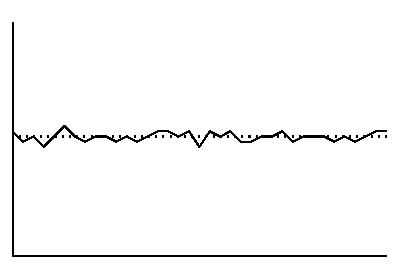
\includegraphics{Figures/energyA}}&
	        \scalebox{0.5}{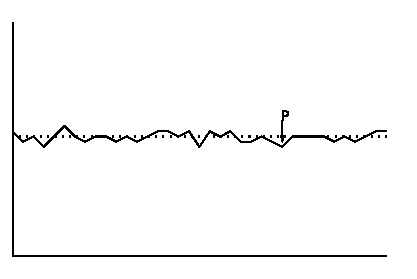
\includegraphics{Figures/energyB}}&
	        \scalebox{0.5}{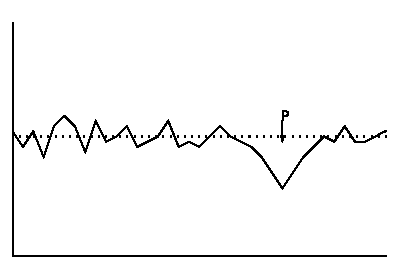
\includegraphics{Figures/energyC}}
				\end{tabular}  
      \caption{Graphs of energy surface during learning.  $A$ before learning, $B$ learnt pattern $p$ with no noise, $C$ learnt pattern $p$ with noise applied to the unit input}
        \label{fig:EnergySurfaceDeltaLearningNoNoise}
  \end{center}
\end{figure}


\subsection{Serial and concurrent learning}   %%%%%%%%
\label{sec:SerialConcurrent}

The Hebbian and delta algorithms highlight an important distinction between different approaches to learning generally, the serial learning of items in a sequence vs. the concurrent learning of a complete population of items.

\term{Serial learning} (also called sequential or ongoing learning) consists of exposure to single items in a sequence, where each item is learnt as well as possible when presented.  It can be used in situations where the training population is not fully known or defined when learning starts -- any time that a new item is presented it can be learnt by the network.  Hebbian learning as described above is an example of an inherently serial algorithm.  Each item is learnt once.  There is no point in repeating items (if for example the whole population was learnt a second time, it would simply double the magnitude of the weights without changing their distribution). Hence the concept of an "epoch" of learning does not apply, and a new item can be learnt by the network at any time.
 
 \term{Concurrent learning} consists of exposure to a complete population of items (one epoch), where each item in the population makes small learning adjustments. Epochs are repeated until the whole population is learnt to criterion.  It can only be used where the whole population of training items is known and available at the time that learning starts -- all items must be available concurrently.  Delta learning has been described above as it is usually applied, as a concurrent algorithm.  The network learns the population in one phase. Once finished, training is then considered complete, and no further items are learnt.

\term{Concurrent learning} is very effective as an applied technology.  Almost all of the most powerful and widely used ANN learning algorithms are instances of this approach.  However, it is a poor model of human learning, which is an ongoing, lifelong process.  We can learn new information at any time and integrate it into what we already know.  Clearly for exploring human memory, \term{serial learning} is the most appropriate framework.  In this paper we therefore \an{NB - make sure that we do!} focus mainly on serial learning, in particular Hebbian learning and a serial application of the (usually concurrent) delta learning algorithm as described below.

\an{Leaving this old note and reply in for now: I think these distinctions are correct and important thing to keep straight in all subsequent discussion, but interested in your comments here!  Now that I look at chapter 4 after Figure 4.1 there is very little that is serial mode delta until the base populations and pseduroehersal stuff that isn't going to be relevant until the second paper.  Hmmmm - pondering}
\si{Indeed we need to keep this straight.  I like the distinction and I think it is important.  I will look as 4 and see what I can do to emphasis the serial nature.  All the work was done with serial learning so I think it is relevant. I compared to concurrent methods merely as a baseline}

\subsection{Measures and assumptions}   %%%%%%%%
\label{sec:measurements}

In this paper we are concerned with measuring and comparing the capacity and stability of different kinds of learning scheme.  Performance and the measurement of performance can only be addressed within the context of a certain set of assumptions about network architecture, parameters, learning algorithms, measurement techniques and so on.  There are a number of different ways to assess a Hopfield type network (or a content addressable memory system in general). For example there are various ways of measuring capacity depending on: the type of pattern stored~\citep{Amit1987b}, the learning procedure~\citep{Storkey1999}, connection symmetry~\citep{Chen2001}, and the definition of successful storage~\citep{Lowe2005}. Different authors use very different measurements which seem to be chosen to best differentiate their network from other solutions (for example compare ~\citet{Christos1996} and \citet{vanHemmen1997}).  In this section we briefly note the range of options, and state our methods and assumptions.

One of the factors affecting capacity is the``activation density" -- the percentage of active units in the patterns learnt.  This has different consequences for  \hopnet{N,\pm}{} and  \hopnet{N,0}{}.  For \hopnet{N,0}{} the use of populations of patterns with a lower activation density makes learning easier and increases capacity, as there is very little information being stored in each pattern. In the limit orthogonal patterns are easily separated.  For  \hopnet{N,\pm}{}, because of the the symmetries noted above, every unit and every weight is significant in every pattern, thus the lowest possible activation density is effectively 50\% (half of the units in each state $<1, -1>$) -- and this is optimal for ease of learning and for capacity.  Similarly, populations where there are systematic relationships between the patterns (such as linear dependencies) can, depending on the nature of the relationships, make learning easier or harder.  For this reason it is common when exploring the properties of these networks to factor out this source of complexity by using randomly structured populations.  Unless otherwise stated, in our simulations we will use \hopnet{N,\pm}{} where patterns are constructed by setting each unit to be active with $50\%$ probability, so that $\percentON=P(x_i=+1)=P(x_i=-1)=0.50$. These are \newterm{independent identically distributed} (i.i.d.) patterns generated by Bernoulli random values.  When distributions other than these are used, they will be noted as $\pattern_{0.2}$ when $\alpha=0.2$, indicating that $20\%$ of the units in the pattern $\pattern_{}$ are active. \an{Do we actually use any variation from 0.5 in the paper?  if not, remove? - but see backrefs to eg start of 3.5}
  

\an{I re-ordered some of this stats stuff so make sure I didn't break anything!  State learning constants and any other practical assumptions here too...}

Given that there are many different criteria by which the efficacy of learning could be assessed, the conventional measure is the number of trained patterns which are stable after learning, as per the original description of Hopfield network capacity~\citep{Hopfield1982}.  After learning the network is assessed by presenting each learnt pattern as an input, and testing to see whether it is stable (do any units change state after a full cycle of unit updates?).  The greater the percentage of the training population which is stable the more effective learning is taken to be.  This \term{recognition capacity} measure is simple to compute and easy to compare across different networks.  Despite the shortcomings described below, for consistency with the existing literature we will use \term{recognition capacity} as our basic measure of performance.

\term{Recognition capacity} is easy to compute and to interpret, but it is a fairly weak measure of ``learning" for a content addressable memory. It is a minimal check of whether each pattern is stable, it says nothing about how easy it is to retrieve patterns from various inputs -- the nature of the basins of attraction. A pattern that is only just stable may be recognised but not recalled from similar content. For a network to be an effective memory recall system there must be a useful number of inputs that relax to learnt patterns. We will call such a measure the \term{recall capacity}.  In this context performance depends on two factors, the number and nature of the basins of attraction of the learnt states, and the number and nature of the basins of attraction of unlearnt but stable (i.e. spurious) states.  

The basin of attraction for a stable pattern is the set of states which relax to that pattern.  The larger the cardinality of the set the greater the size of the basin.  In the \hopnet{6,\pm}{} network above with one learnt pattern, the two stable states (the pattern and its inverse) have large basins (Figure \ref{fig:EnergySurfaceHopnet}).  As the number of patterns learnt by the network increases the size of the basin of each individual pattern decreases, and the number of spurious stable states increases.  These are both very important factors when using the Hopfield network as a CAM (content addressable memory).  If a learnt pattern is to be recalled from a noisy version of the pattern, the noisy input has to be within the basin of attraction of the target learnt pattern.  If the basin is too small then very few patterns will relax to the target (those that start with almost identical unit activations).  When the learnt patterns no longer have basins of attraction at all the memory system is only useful testing familiarity, not recall.  If there are too many spurious states with significant attractors then these can obscure or eliminate the learnt states altogether.  Ideally a CAM will avoid both of these problems, having all learnt patterns stable with large basins of attraction, and few or ideally no spurious stable states. 
 
Assessing \term{recall capacity} is a complex task which involves ``probing" the network with many random inputs, recording the final stable states which they relax to, and gathering statistics on the number of input probes which relax to each stable learnt or spurious state.  For a network with any significant number of units the number of possible input states is huge, hence it is impossible to probe the network exhaustively, and for larger networks \term{recall capacity} estimates become increasingly approximate.
 
\an{;;; could do more here - thesis subsections 2.5.2 Basin size and 2.5.3 Hamming distance?  ALSO 2.4.6 on update timing probably here.  later: No - it's already too big!  But leave this note in for now and ponder.}
%2


\subsection{Maximum capacity}   %%%%%%%%
\label{sec:capacity}

\an{incorporated stuff from previous 4.2.1 - needs checking}

The number of patterns that can be learnt by a Hopfield type network is limited by the amount of information that it can store. Different populations of patterns contain different amounts of information depending on their activation density and their structure. Randomly generated patterns contain a large amount of information as estimated using either Kolmogorov complexity or Shannon information theory (for and in depth coverage of information theory see \citet{Cover1991}). Information based on probability theory in this context can be described as, how surprising an activation of a unit is, given the previous set of patterns.  For binary units the maximum amount of information is where each pattern has $50\%$ of its units active.

For this reason computations of the capacity of Hopfield networks typically employ uncorrelated patterns where the probability of each unit being active is $50\%$, i.e. $\pattern_{0.5}$ as described above.  A recognition measure of capacity is also typically assumed.  Under these conditions the theoretical maximum number of patterns that can be stored in a Hopfield network, independent of the learning rule, is $\hopnetcapacity=N$ patterns for networks with symmetric connections, and $2N$ for asymmetric connections~\citep{Gardner1988}.  The actual capacity of a given network depends on the specific learning algorithm and parameter settings.  
 
Considering specific learning algorithms, the most widely cited result is for Hebbian learning.  The original estimation was $\hopnetcapacity = 0.14N$~\citep{Amit1987}, where $N$ is the number of units in the network. Rigorous mathematical proofs~\citep{McEliece1987,Bovier1999,Lowe2005} have shown that the upper bound for perfect recall is actually closer to:
\begin{equation}
\label{eq:HopnetcapHebbian}
	\hopnetcapacity = \frac{N}{\gamma \mbox{ln} N}
\end{equation}
where $\gamma = 2,4,6$ depending on the exact dynamics of the storage required.  These results assume independent identically distributed (i.i.d.) patterns (as described above) for \hopnet{N,\pm}{}.  

The delta learning algorithm, as usually (concurrently) applied, is the most powerful learning algorithm available for Hopfield type networks.  
Under ideal circumstances its practical performance approaches the theoretical maximums of $N$ patterns for networks with symmetric connections, and $2N$ for asymmetric connections. \an{hope that's all true!}  
As stated above, however, for the purposes of modelling human memory we are particularly interested in serial learning approaches.  
For this reason we will use the delta rule in serial or partly serial tasks.  In a completely serial task the delta rule can be used to learn each item individually when it is presented, i.e. in a single sequence, as is the case for Hebbian learning.  We are not aware of any formal calculation of the capacity of delta learning when used in this way, but empirically we have found it to be similar to that of Hebbian learning ($0.14.N$) as described below. \an{I think we need to do this as a baseline demo - note at that point that each item is learnt repeatedly if necessary until it is learnt to criterion}.

In the remainder of this paper, and in the related \citep{McCallum2010b}, we explore ways in which various modifications to the basic learning algorithms can increase their capacity.


\newpage{}%%%%%%%%%%%%%%%%%%%%%%%%%%%%%%%%%%%%%%%%%%%%%%%
\section{Capacity, stability and the dynamics of learning}
\label{sec:StabilityDynamics}

The issue of learning in a dynamic environment, including such topics as serial learning (where information arrives in separate episodes over time) and conceptual drift (where the relevant training population changes over time) represents a serious challenge for any learning system. Ideally the representations developed should be stable enough to preserve important information during new learning, but plastic enough to incorporate new information when necessary. These requirements constitute the stability / plasticity dilemma ~\citep{Grossberg1987} -- both stability and plasticity are desirable, but their requirements are in direct conflict.

Humans and other animals have clearly evolved mechanisms which manage this dilemma, and are capable of successful learning as a serial, ongoing, lifelong process.   In contrast ANNs as learning systems are, as discussed below, generally poor at learning in this way.  It is in this context that the specific issues of the capacity and stability of learning in Hopfield networks are of particular interest.  

Serial learning in Hopfield type networks (using Hebbian or Delta learning) has a low maximum capacity, and the performance of the network degrades as learning continues -- these are the first and second problems for Hopfield networks as memory systems as noted in the Introduction.  In this section we explore the dynamics of ongoing learning in these networks, looking in detail at their performance and stability over extended serial learning, the causes of their collapse in capacity, and simple techniques for mitigating this collapse and increasing capacity.

\subsection{Catastrophic forgetting}  %%%%%%%%
\label{sec:CF}

Before focusing on Hopfield networks it is useful to briefly consider the performance of ANNs in general. Most learning algorithms do not manage the stability / plasticity dilemma well.  In particular, they are prone to catastrophic forgetting (CF), the sudden and total loss of previously learned information when new learning occurs.  Grossberg suggests the analogy of a human trained to recognise the word ``cat'', and subsequently to recognise the word ``table'', being then unable to recognise ``cat''.  

CF has been identified in many forms in the ANN literature, and has also been called the ``catastrophic interference'' or ``serial learning'' problem~\citep{Hetherington89, McCloskey1989, Lewandowsky91, French1992, McRae1993, Sharkey1995, Robins1995, French1999, Ans2002, Robins2004}.  CF has most often been explored in the context of multi-layer perceptron (MLP) type architectures~\citep{McCloskey1989, Hetherington89, Ratcliff90, Lewandowsky91, Murre1992, French1992, French1994, French1997, McRae1993, Lewandowsky1995, Sharkey1995, Robins1995, Robins1996, Frean99}. The standard demonstration of the effect uses an MLP that has been trained on a ``base'' population, and then tests performance once a new item or group of items has been learnt.  Typically the recall of the base population falls off very sharply.  This CF can occur with only a single new item learnt.

CF in this kind of network arises because of unmanaged plasticity.  New learning changes the weights which embodied the information previously learnt by the network, thus disrupting performance on old items.  This is the (seldom acknowledged) reason that most ANN learning algorithms are concurrent, so that the whole population of interest can be learnt over multiple epochs, each time repairing the damage that the individual items cause each other during learning, until a set of weights can be found which works for all items.  In contrast serial learning is inherently vulnerable to CF.  Items which are learnt early are almost always damaged by later learning.  

In earlier work we have explored CF in MLPs and proposed the pseudorehearsal mechanism ~\citep{Robins1995}. Pseudorehearsal uses random samples of the input-output behaviour of a network in a rehearsal process to protect the base population as new items are learned.   This is an effective mechanism and pseudorehersal has become the preferred solution to CF in this kind of network, many instances of its application are reviewed in ~\citet{Robins2004} \an{New ref:  Robins, A. Sequential learning in neural networks: A review and a discussion of pseudorehearsal based methods. Intelligent Data Analysis, 8(3), 301 - 322 (2004)}.  Having established a suitable foundation of underlying issues in the current paper, we explore the topic of pseudorehearsal in Hopfield networks in detail in ~\citet{McCallum2010b}.

\subsection{Capacity and the causes of forgetting}  %%%%%%%%
\label{sec:ForgettingCapacity}

Catastrophic forgetting (CF) is also an issue for learning in Hopfield type networks, as is shown in \citet{Robins1998}.  Similar issues have been explored by \citet{Nadal1986} and \citet{Burgess1991}, and in the context of the ``unlearning'' mechanisms \an{cite unlearning refs}.  In this kind of network CF is not a discrete issue, a simple consequence of unmanaged plasticity, as it is in MLPs (where it is masked by concurrent learning).  In Hopfield networks forgetting arises from the complex interaction of fundamental issues of maximum capacity, population structure and unconstrained plasticity within the context of a serial learning task.  Our initial exploration of CF and the pseudorehearsal solution in Hopfield networks ~\citep{Robins1998} was blind to these complexities, which we now explore in the subsections below.  

\subsubsection{Catastrophic capacity}
\label{sec:CatastrophicCapacitySol}

\an{ultra condensed from previous version - please check!}

As noted in Section \ref{sec:capacity} above, the number of patterns that can be learnt by a Hopfield type network depends on the population's activation density and structure.  Under the typical assumptions where patterns are random and probability of each unit being active is $50\%$, the upper bound for Hebbian learning is roughly $0.14N$. It is an upper bound precisely because above this limit Hebbian learning exhibits a particularly severe form of CF where the performance of the network collapses.  Crosstalk in the input population overwhelms the ability of the network to distinguish patterns as discrete entities \an{ref to e.g. Hertz Krough and Palmer?}.  Rather than losing just the old material the network can spontaneously lose all stored patterns including, the new items.  This can be caused by a single global spurious attractor taking over the whole space with a global basin of attraction, or by the generation of thousands of small attractors (stable states with a basin of attraction).  

The catastrophic loss of pattern stability is shown in Figure~\ref{fig:hebb64clean} \an{where is this figure?} for a network of 100 units.  The line shows the average over 100 repetitions with error bars extending to one standard deviation. This network shows classic CF under the pressure of capacity.  The storage of this $100$ unit network \(\hopnet{100,\pm}{}\) from equation~\ref{eq:HopnetcapHebbian} is approximately 14 patterns.  Note that by the time 18 patterns have been presented the likelihood of a learnt pattern being stable is about $50\%$ (9 patterns are stable on average).  As more patterns are presented fewer and fewer of them remain stable in the network.  

\begin{figure}[tbp]
\small
\center
	\begin{center}
%		\input{Figures/Hebbian/HopCF.tex}
	\end{center}
	\caption{Number of trained patterns stable in a 100 unit Hopfield network \hopnet{100,\pm}{} with Hebbian learning showing CF (averaged over $100$ repetitions, 50\% random patterns).}
	\label{fig:hebb64clean}
\end{figure}

\an{NBNB - need to repeat the above or very similar for plain serial delta learning as per discussion above}

Because the performance of Hopfield type networks becomes pathological at the limits of capacity, it is important when developing solutions to CF to evaluate them in networks which are far from capacity as well as those which are close to their theoretical limits.

;;; working point here ;;;

\subsubsection{Catastrophic correlation}
\label{sec:CatastrophicCorrelation}

\an{Currently just a copy and paste of thesis 4.2, will need consistency checking and probably trimming for size}

Most of the capacity measures for Hopfield networks involve the analysis of uncorrelated random patterns (independent identically distributed random variables -- i.i.d.).  Assuming that all the patterns that need to be learnt will come from these sorts of clean distributions is unrealistic.  Patterns from real data sets are likely to have correlations, and in fact it is likely that it is the correlations between events that makes it possible to extract causal relationships.  Correlations alter the analysis of capacity: 1) the maximum theoretical capacity increases in relation to the amount of overlap and the nature of the correlation~\citep{Gardner1988, Lowe1998, Gandolfo1999, Kimoto2002, Bogacz2003}, and 2) Hebbian learning performs poorly with correlated patterns as the crosstalk term becomes very large and the pattern which is the correlation between inputs becomes the only stable attractor.

To understand why correlation increases the number of patterns that can be stored, the amount of information in each pattern must be analysed.  In the extreme case of only one unit being active in each pattern it is easy to see how to store any of the $N$ ``one unit active'' patterns.  To store these patterns the connections between units are set to a negative value so that active units tend to deactivate other units, and the unit that is active in a pattern has a positive connection from the bias unit so that if it is active it remains active.  This easy solution for storing $N$ patterns is a result of each pattern only having a small amount of information.  Because of the symmetry in binary activation, patterns with all but one unit active contain the same amount of information as patterns with only a single unit active.  

\citet{Amit1987b} argue that Hebbian learning can be altered to accommodate correlated patterns where the correlation is caused by a low coding ratio (only a small percentage of the units are active).  The learning rule can be changed to:
\begin{equation}
	\label{eq:HebbianlearningCorrellated}
	\delta\weight{ij} = (\unitActivation{i}{}-\alpha)(\unitActivation{j}{}-\alpha)
\end{equation}
where $\alpha$ is the sparseness of the coding.  This concept of correlation caused by a uniform decrease in the number of units that are active is useful only when the patterns have a known activity level and that activity level is the {\em only} correlation between the learnt patterns.  The patterns themselves need to be uncorrelated in terms of which units are active for this approach to work.

Correlation does not come from just a change in the coding ratio for the patterns.  One interpretation for correlated patterns is the concept of a prototype.  The prototypical car will have many features in common with individual cars.  A learning set that contains groups of similar objects will have correlated patterns and the combination of these correlations may be the prototype for the group.  

Hopfield networks with Hebbian learning cannot make highly correlated patterns stable.  Instead a pattern which is the combination of the learnt patterns will become a stable state with a large basin of attraction.  There are two types of correlation, one caused by a low coding ratio where the patterns are still independent, and correlation caused by patterns which share a large number of features. The difference can be most clearly demonstrated with an example. 

In this example the learning population is generated by making small perturbations of a checkerboard pattern (Figure~\ref{fig:checkerpert}).  These patterns have a coding ratio of about $50\%$ but are also extremely highly correlated.  This form of correlation immediately destroys the basin of attraction of the individual patterns and the only attractor is the correlated prototype, in this case a checkerboard pattern.  To show this, consider three patterns that are based on a checkerboard pattern with $k$ units altered $(k<<N)$ with alteration ratio ($\alpha_{a}$) $= k/N$ .  Having learnt three patterns there are four catagories of units representing the different types of overlap of the perturbed checkerboard patterns.  The average number of units in each set (cardinality C), can be calculated from the alteration ratio $\alpha_{a}$
\begin{enumerate}
\item The set of units altered in all three patterns. \\
  \hspace{1cm}$\Phi^{3}_{3}=\phi_{1\wedge2\wedge3}$, \\
  \hspace{1cm}$C = \alpha_{a}^3$
\item Units altered in two of the three patterns. \\
  \hspace{1cm}$\Phi^{3}_{2}=\phi_{1\wedge2}+\phi_{2\wedge3}+\phi_{1\wedge3} -
  \phi_{1\wedge2\wedge3}$, \\ 
  \hspace{1cm}$C = 3*(\alpha_{a}^2*(1-\alpha_{a}))$
\item The set of units altered in just one pattern. \\
  \hspace{1cm}$\Phi^{3}_{1}=(\phi_{1} +\phi_{2} + \phi_{3})   
  -(\phi_{1\wedge2}+\phi_{2\wedge3}+\phi_{1\wedge3}+\phi_{1\wedge2\wedge3})$, \\
  \hspace{1cm}$C = 3*(\alpha_{a}*(1-\alpha_{a})^2)$
\item The set of units that conform to the checker board in every learnt pattern.\\
  \hspace{1cm}$\Phi^{3}_{0}=N-\phi_{1\vee 2\vee 3}$, \\
  \hspace{1cm}$C = (1-\alpha_{a})^3$
\end{enumerate}
where $\phi_{1\wedge2\wedge3}$ is the set of units whose activation was altered in all the patterns 1, 2 and 3;
 $\phi_{1\wedge2}$ is the set of units altered in patterns 1 and 2;
 $\phi_{1}$ is the set of units altered in patterns 1; and
 $\phi_{1\vee2\vee3}$ is the set of units altered in pattern 1, 2 or 3.

\begin{figure}[tbp]
\small
\center
	\begin{center}
		
\includegraphics{Figures/checkerboard}
	\end{center}
	\caption{Checker board with two possible perturbations $A$ and $B$.}
	\label{fig:checkerpert}
\end{figure}

If the altered units are selected from an i.d.d.\ at random then $\Phi^3_{3}$ would have cardinality $\approx \alpha_{a}^3*N$.  Given small $k$, the number of units altered in more than one pattern is very small.  A unit $i$ selected at random from the set of units in $\Phi^{3}_{1}$ will have connections to units $j$ in $\Phi^{3}_{0}$, each with a weight $\weight{ij}=1$ giving a net input to the unit of $N*((1-\alpha_{a})^3)$.  Given that the units in the other categories have at most $\weight{ij} = \pm3$ so long as $\alpha_{a} < 0.14$ for three patterns and $\alpha_{a} < 0.22$ for four patterns, the unit will change state to match the checker board.  The more patterns which are learnt from the set of patterns with minor alterations to the checker board pattern, the larger the prototype's basin of attraction becomes.  

If the units in the pattern are slowly ``fatigued'', where their input is lowered by a set amount, after several iterations individual patterns emerge from the prototype. This is because the units that were altered in the learnt patterns are closer to threshold than the units that are only in the checker board pattern.  The major problem with this is that the patterns generated by this process of fatiguing the units are not just the learnt patterns, but include many spurious patterns.


\subsubsection{Catastrophic plasticity}
\label{sec:CP}

\an{Currently just a copy and paste of thesis 4.3, will need consistency checking and probably trimming for size.  Also need to be focused on serial mode rather than concurrent, if not possible will have to rethink whole emphasis on serial!!!}

Catastrophic forgetting in Hopfield networks with Hebbian learning is mainly attributable to capacity and correlations.  However by using delta learning both the catastrophic correlation and catastrophic capacity problems  are reduced.  Delta learning deals with correlation by only making changes that improve performance, and the capacity is increased dramatically to close to the theoretical information capacity of the network.  

However delta learning in Hopfield networks also suffers from excessive plasticity.  Delta learning is able to learn a larger number of patterns by slowly adjusting the weights until they make the current set of patterns stable.  Thus when learning new patterns, all the weights are changed to match the new patterns.  This plasticity, the key to the power of the learning algorithm, can cause catastrophic forgetting.
 
As discussed in \citet{Robins1998} there is a great deal of similarity between the CF caused by excessive plasticity in MLP networks and in Hopfield networks using delta learning. Figure~\ref{fig:HOP-CP} shows the number of base population patterns that become unstable as new patterns are learnt.  It is this type of CF that is the target of the pseudorehearsal solution presented below in Section~\ref{sec:PRSolution}.

\begin{figure}[tbp]
\small
\center
%		 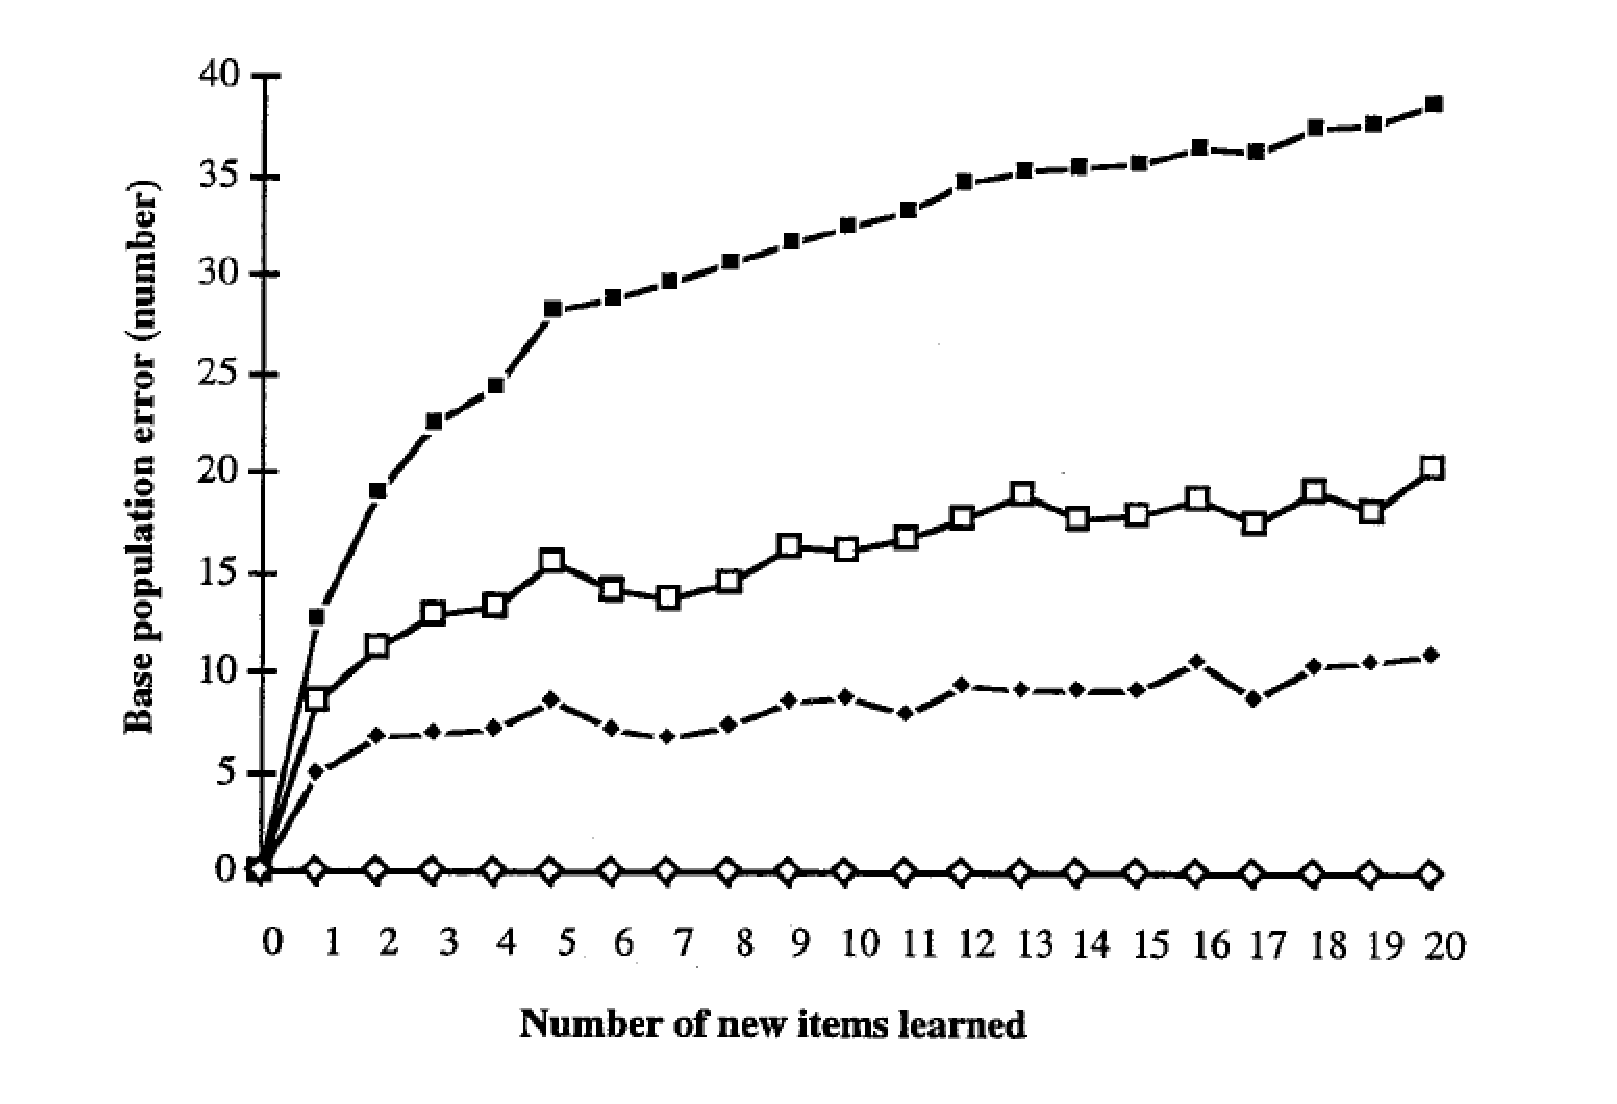
\includegraphics[width=0.90\textwidth]{Figures/HOP-CP} %\input{Figures/HOP-CP} %
	\caption{Catastrophic forgetting in a Hopfield network caused by plasticity (adapted from Robins and McCallum (1998) Figure 4).}
	\label{fig:HOP-CP}
\end{figure}

\subsection{Hebbian learning}  %%%%%%%%
\label{sec:hebbianSolutions}

How do these issues play out in the context of Hebbian learning.  What kinds of simple solutions are available? \an{;;; expand!}

As reviewed above, CF does not have a single cause, and although the various solutions tend to focus on a particular cause, they usually have an affect on all of them.  For example, the unlearning mechanism of \an{cite Hopfield and Crick, Christos, van Hemmen etc} was initially designed to solve the problem of the limited capacity of Hopfield networks, but later analysis showed that it was also affecting the problem of catastrophic correlation~\citep{Christos1996}.  The complexity of the interactions between the solutions and the various types of problems makes it difficult to directly compare solutions.  Each solution makes trade-offs between plasticity and stability, complexity and robustness, and biological plausibility.  

in the remainder of this paper we explore simple solutions, in \cite{McCallum201b} we explore more complex solutions such as unlearning and PR. \an{expand "simple" and "complex" - stopping here damn got to go! ;;;X }

\an{Currently just a copy and paste of bits of thesis 4.4, will need consistency checking and probably trimming for size}

\subsubsection{Weight decay}

Weight decay is one of the simplest post--processing operations to implement.  After each item, or set of items, are learnt every weight in the network is multiplied by a value just less than 1.  This reduces the magnitude of each weight, moving it closer to 0.  As Hebbian learning alters the weights by a fixed amount, it is easier to learn a new pattern when the weights are small.   There is also biological evidence of a decay mechanism which reduces and even eliminates connections over time.  There appears to be two types of LTP(long term potentiation), decremental and persistent~\citep{Abraham2003}.  Hebbian learning with weight decay would be equivalent to decremental LTP.  

This can be considered a form of \term{managed forgetting}, where the forgetting of previous information is included in the learning algorithm.  Using weight decay it is possible to calculate the influence on each weight that an old learnt pattern will have, directly from the number of patterns that have been learnt since it was presented.  With weight decay of $\weightDecay = 0.1$ after 10 additional patterns have been learnt, the contribution of the original pattern will be $0.9^{10} = 0.35$ of that pattern's original contribution.  This controlled forgetting allows weight decay to avoid CF. 

\citet{Christos1996} showed that weight decay is able to reduce the CF caused by overloading the network, at the cost of lowering the effective capacity to $0.05N$.  Figure~\ref{fig:WeightDecay100num} shows our comparison between normal Hebbian learning and learning with a weight decay of $\weightDecay = 0.1$. The weights are each new pattern are altered so that $( w_{ij} = w_{ij}*(1-\weightDecay))$ (see Appendix \ref{app:weightDecay} for other parameters used for this simulation).  The CF of the standard learning system can be clearly seen when the network learns more than $\approx 0.14N$.  However, using weight decay the system is able to retain about $0.07N$, slightly above the estimate of $0.05N$ by \citet{Nadal1986}.  The patterns that are stable in this network are the most recently stored patterns.  Although stable, the basin of attraction of the oldest stable pattern is very small. Most of the random probes of the network fall within the basin of just the most recently learnt pattern.  Figure~\ref{fig:WeightDecay100pos} shows the probability with which a pattern is stable after learning multiple patterns using Hebbian learning and weight decay of $\weightDecay = 0.1$. This graph shows that after learning 20 patterns, the 15th pattern that was learnt was stable in about $70\%$ of the 100 trials. The fall off from 100\% stable for the last two or three patterns learnt to never stable is similar for each of the three conditions shown. 

\begin{figure}[tbp]
\small
\center
%	\includegraphics{Figures/Hebbian/WeightDecayHop}
	\caption{Number of trained patterns stable in a 100 unit Hopfield network \hopnet{100,\pm}{} with Hebbian learning and weight decay $\weightDecay = 0.1$ per item (averaged over $100$ repetitions, with error--bars showing standard deviation).}
	\label{fig:WeightDecay100num}
\end{figure}

\begin{figure}[tbp]
\small
\center
%	\includegraphics{Figures/Hebbian/hebbianRecallWdecay}
	\caption{Probability of a learnt pattern being stable based on when it was learnt.  Probabilities are shown after 10, 20, and 30 patterns have been learnt in an \hopnet{100,\pm}{} network with Hebbian learning and weight decay of $\weightDecay = 0.1$ per item ($100$ repetitions).}
	\label{fig:WeightDecay100pos}
\end{figure}

As noted by \citet{Christos1996} it may seem better to learn $0.14N$ patterns and then wipe the network clean and learn the next set of $0.14N$ patterns.  This ``manages'' the forgetting by removing all the patterns and working with a clean network to learn new information.  This does allow new patterns to be learnt continually over time, but at the cost of catastrophic removal of all previously learnt information every $0.14N$ patterns.  Christos suggests that the reason that this is not a viable solution is the lack of a biological analogy, but there is also the problem that when averaged after each pattern is learnt the number of patterns stored is only $0.07N$.

Weight decay provides a simple and successful solution to the problem of CF.  This success however results in a network with a very low \emph{recognition capacity}, and an even smaller \emph{recall capacity}.  When probed, the network almost always returns only the most recent pattern, and the older patterns fade very quickly.  However weight decay will be important in analysing the behaviour of other solutions as it provides not only a base performance level, but also appears be the main cause for the improved performance of other systems such as unlearning, a possibility discussed later in this chapter.

\subsubsection{Weight capping}

\citet{Willshaw1969} showed that perceptron networks with only three possible connection values; -1, 0, +1 were able to solve a variety of problems. Surprisingly when a Hopfield network has the weights capped to a low value, it ameliorates some of the problems of CF. Figure~\ref{fig:WeightCap100num} shows the result of five different capping values.  With a learning constant of $\learningConst = 1$ the condition labelled ``1'' matches the Willshaw model capped at 1 and -1.  In an \hopnet{100,\pm}{} the best results are achieved with a capping value of $3$ (7 different weight values).  The performance of weight capping is only slightly below that of weight decay.  As with weight decay, weight capping can be justified from a biological perspective.  The cap represents a constraint on the maximum efficacy of a synapse between two neurons.

The similarity between weight decay and weight capping may not be obvious at first, but when inspecting the weight changes it becomes clearer.  The effect of weight decay is to bring the weights closer to zero which allows the Hebbian learning rule to make a large enough change to the network to make the new pattern stable.  Using a very low weight cap the weights can never move far from zero, and so the large correlations that normally cause CF are removed.  The combination of weight capping and decay does not provide a cumulative performance improvement as the two approaches solve the same problem in similar ways. Both of these systems perform well, and in combination with their biological plausibility, they provide a solid lower bound to assess the more complex solutions.  

\begin{figure}[tbp]
\small
\center
%	\includegraphics{Figures/Hebbian/WeightCapHop}
	\caption{Number of trained patterns stable in a 100 unit Hopfield network \hopnet{100,\pm}{} with Hebbian learning and weight capping values 1--5 ($100$ repetitions, N.B.\ error bars removed for readability).}
	\label{fig:WeightCap100num}
\end{figure}

\subsubsection{Other}

There are many alterations to the basic Hebbian learning rule to try to make it either more biologically plausible, or more effective. \citet{Dayan1991} showed that for catastrophic correlation caused by a low coding ratio the best learning algorithm was the one suggested by \citet{Amit1987b} (see Equation:~\eqref{eq:HebbianlearningCorrellated}). A similar result was achieved by \citet{Palm1996} by changing the activation values of the units so that instead of $(1,-1)$ or $(1,0)$ the output was $(1,-a)$ where $a = \alpha/(1-\alpha)$ ($\alpha$ is the coding ratio).  Thus, with 50\% of the units active, as is the case with most of the examples in this thesis, the activation values are $a=0.5/(1-0.5) \rightarrow (1,-1)$.  Both of these solutions solve the problem of catastrophic correlation for patterns with low coding ratio.  They do not however solve CF which still limits Hebbian learning.  \an{last sentence needs rephrasing, which aspect of CF remains unsolved?}

A variety of other methods are based on explicit normalisation (using information that is available locally at the level of the unit). \citet{Chechik2001} describe a mechanism for normalising the inputs to each unit so that the sum of all the connections is zero.  The problem that \citet{Chechik2001} were focused on was the issue of catastrophic correlation when learning patterns with low coding ratios.  The large number of inactive units tends to overwhelm any individual active units and the patterns become difficult to learn.  

The contribution of \citet{Chechik2001} was to show that a local neuron level alteration could achieve a similar result to the learning rule change suggest by \citet{Amit1987b}(see Equation:\eqref{eq:HebbianlearningCorrellated}) without having to pre-calculate the coding ratio.  This normalisation process equalises the weight changes so that the simple Hebbian learning rule is still able to learn patterns which have a low coding ratio.  This form of zero sum normalisation does not alter the performance of Hebbian learning in the $\alpha =50\%$ space and so CF caused by capacity is still a problem, see Figure~\ref{fig:WeightNormZM100num}.  With the low $\alpha$ patterns this zero sum normalisation returns the performance to that of the learning rule in Equation~\eqref{eq:HebbianlearningCorrellated}.

\citet{Horn1998a} developed a system to regulate the connections to units in terms of the unit's activation in the learnt patterns.  Like the normalisation process above, this ``neuronal regulation" is designed to improve the performance with sparsely coded patterns.  The principle is to change the weights that contribute the most strongly to a set upper bound, and to set the weights below a threshold to zero.  This simplifies the possible values of weighted connections, and removes small amounts of noise.  In our simulations this process improved performance on sparsely coded networks but not significantly more than other methods.  The main justification for using this model is the biological plausibility of the modelling and the improvement in the basins of attraction of the learnt patterns. 

Further explorations of normalisation and resource limitation techniques are described in \citet{McCallum2007} \an{need a new reference for your thesis!}.  In general the performance of these methods is similar to the $0.07N$ limit of the simpler mechanisms of weight capping and decay.  \an{May want to expand slightly with material from thesis 4.4.2 depending on overall length}.

\subsection{Delta learning}  %%%%%%%%
\label{sec:deltaSolutions}

How do these issues play out in the context of Delta learning.  What kinds of simple solutions are available? \an{;;; expand! - be clear on concurrent vs serial delta}

\an{Currently just a snip of thesis 4.4.7}

Delta learning in Hopfield networks does not suffer from catastrophic forgetting in the same way as unmodified Hebbian learning.  Figure~\ref{fig:Delta-WeightDecayComp} shows the performance of delta learning against Hebbian learning with weight decay.  The performance of delta learning is slightly better than that of weight decay, and there is not the total loss of functionality that results from unmodified Hebbian learning.  In the network that generated the data for Figure~\ref{fig:Delta-WeightDecayComp}, new patterns were learnt one at a time for a maximum of 5000 epochs or until the error was less than $0.001$.  The network required, on average, only $711\ (stddev=34.94)$ epochs to learn each new pattern (100 items for 100 repetitions, giving 10,000 data points for this average).  The maximum time taken was only 1489 epochs, so at no stage did the learning stop because of the epoch limit.  The patterns were learnt with absolute Gaussian noise\footnote{Gaussian noise as described in Section~\ref{sec:learningAlg}.} (\noiseConst{i}) of $0.5$ applied to each unit in each epoch of learning.  This noise helps to make the learnt patterns more robust and to create a basin of attraction around the new pattern.

Adding weight decay to delta learning does not improve performance.  Weight decay increases the speed at which older patterns are forgotten, and so although it does very slightly decrease the number of epochs required to learn new patterns it is not beneficial to the overall capacity of the network. 

\begin{figure}[tbp]
\small
\center
	
\includegraphics{Figures/empty}
%	\includegraphics{Figures/Delta/Delta-WeightDecayComp}
	\caption{Number of trained patterns stable in a 100 unit Hopfield network \hopnet{100,\pm}{} with delta learning versus Hebbian learning with weight decay $\weightDecay = 0.1$ per item ($100$ repetitions).}
	\label{fig:Delta-WeightDecayComp}
\end{figure}

As discussed in Section~\ref{sec:deltaLearning} delta learning in MLP networks introduces its own type of catastrophic forgetting -- catastrophic plasticity, caused by excessive change of the weights to accommodate a new pattern.  This also occurs in Hopfield networks. The forgetting of the base population is seen in Hebbian learning with weight decay, but the forgetting is gradual and continuous rather than catastrophic.  The difference between the two is partly due to the low capacity of Hebbian learning.  With delta learning, the number of patterns that can be stored in the network is much larger than with Hebbian learning, so when new patterns are learnt there is more to lose.  The ongoing performance of delta learning and Hebbian learning in Figure~\ref{fig:Delta-WeightDecayComp} is similar.  However, delta learning has a much higher possible capacity than Hebbian learning, and it is when patterns are learnt in blocks that both the higher capacity and catastrophic plasticity become evident.

Figure~\ref{fig:CFDelta} shows CF caused by the plasticity of the delta rule.  The gradient of the forgetting caused by learning new patterns is related to the number of patterns in the base population.  The larger the number of patterns learnt, the more fragile the learning.  This is a result of the balancing that delta learning does to make multiple patterns stable.  Delta learning is able to make $0.9N$ patterns stable, but after just ten more patterns are added its performance is down to only $0.05N$ patterns. This massive loss of stored information is the CF that we will try to prevent when using this algorithm.

\begin{figure}[tbp]
	\small
	\center
	
\includegraphics{Figures/empty}
%		 \includegraphics{Figures/Delta/DeltaCF}
	\caption{The number of patterns stable in a 100 unit Hopfield network \hopnet{100,\pm}{} with delta learning of a base population of 30 $(0.3N)$, 60 $(0.6N)$, and 90 $(0.9N)$ patterns followed by learning of new patterns ($100$ repetitions).}
	\label{fig:CFDelta}
\end{figure}

It is possible to combine delta learning with weight decay, weight capping, and neural regulation.  Both weight decay and weight capping degrade the performance of delta learning.  Weight decay just degrades previously learnt patterns faster, and weight capping forces delta learning to spread its changes across more weights and thus degrade previous patterns.  Neural regulation also decreases the weights independently of delta learning.  This decrease of weights again degrades the stability of previously learnt patterns.  Unlike Hebbian learning, delta learning does not need an explicit process to remove old patterns, as it will continue to learn until the new pattern overrides the previous weights.  These systems that control the forgetting of old patterns, do not improve the capacity of delta learning.


\subsection{Discussion}

We've dealt with issues relating to the first and second problems (capacity and stability over time) identified in the introduction.

Any general roundup on cognition and memory. \an{expand}


\newpage{}%%%%%%%%%%%%%%%%%%%%%%%%%%%%%%%%%%%%%%%%%%%%%%%
\section{Learned and spurious states}
\label{sec:States}

Having explored issues of capacity and stability, the third major problem for Hopfield networks as models of memory is that they become cluttered with spurious states.  These are states which were not learnt but which are stable (energy minima).  Some spurious states are obvious combinations of learnt states, some are effectively randomly structured.  Beyond a very light loading, the states learnt by a network quickly come to be outnumbered by the spurious states, often by an order of magnitude or more. \an{all that true?}

Historically there has not been any way of determining whether a given stable state is learnt or spurious (other than comparing it to an external list of learnt patterns, a brute force approach which makes the network completely redundant as a memory system!).  All stable states are treated as if they are equivalent, a pattern of activation to be read off the units.  Any given stable state may be a learnt or it may not.  In terms of modelling human memory, this corresponds to a memory system that cannot distinguish between fact and fantasy.  

In this section we explore the role of spurious states in limiting capacity and in CF.  We summarise various partial methods for distinguishing between learnt and spurious states, and the robust and effective method first proposed in \cite{Robins2004}.  In \cite{McCallum2010b} we build on this foundation, exploring more complex methods of increasing the capacity and stability of Hopfield networks, and showing how the ability to distinguish different kinds of state / attractor allows us to further improve these methods in some cases.

\subsection{Spurious states}  %%%%%%%%

\an{almost verbatim snip}

Spurious states are defined as the stable states in the network that are not part of the trained set of patterns.  In the \hopnet{6,\pm}{} example above, with one pattern learnt, the only stable state was the learnt pattern and equivalently its inverse.  For Hebbian learning if more than two patterns are learnt, spurious states are created.  As the number of learnt patterns increases the number of spurious patterns also increases at a much faster rate.  Once the network has learnt more than the maximum capacity $(0.14N)$, spurious states start to dominate the networks and the learnt patterns are lost.

The spurious states that are generated initially from the learnt patterns are not just random states.  When the number of learnt patterns is small $<<0.14N$ the spurious patterns generated are combinations (crosstalk \crosstalk{i}) of the learnt patterns~\citep{Amit1987}.

\begin{equation}
	\label{eq:crosstalk}
	\displaystyle \crosstalk{i} = \frac{1}{N}\sum_{{j \\ (j \ne i)}}\left( \sum_{p,q (p\ne q)} 		\unitActivation{i}{p}\unitActivation{j}{p}\unitActivation{i}{q}\unitActivation{j}{q}\right)
\end{equation}
Equation~\eqref{eq:crosstalk} describes the interaction of patterns that create crosstalk, which can overload the networks when many patterns are learnt.

\an{This could use expanding a bit.  Is there any content I've missed here on the nature of spurious states, their:
- nature (half way ones and completely random ones)
- frequency (rate at which they are generated as learning a sequence)}


\subsection{Spurious states and recognition} 
 %%%%%%%%  Spurious but looking at stable states / recognition / familiarity

As discussed above (Section~\ref{sec:measurements}) the typical basic measure of the performance of a network is \term{recognition capacity}, the number of trained patterns which are stable when presented as inputs.  However, as a measure of the utility of a practical working memory system this measure has a crucial flaw.  It doesn't take any account of the number of unlearnt patterns which are also stable.  In the pathological case where every state of the network was stable, \term{recognition capacity} would be assessed as 100\%, but the memory system would be completely unable to distinguish between those patterns that it had learnt and those it had not\footnote{Such pathological cases do exist.  For example given the constraint that patterns have exactly 50\% of their units active, all possible patterns are stable in a network with all weights set to $-1$.}.  It would ``recognise" everything, and therefore nothing.

The more a network becomes populated with stable spurious states the more false positives it will generate in recognition tests, and the lower its utility as a practical memory system.  A network that is densely populated with spurious states approaches the pathological condition described above.  Hence the number of spurious states created by any learning in a network is a critical property of the learning process.  The fewer spurious states the better.

The other way in which spurious states can affect recognition is the much more common pathological case of a catastrophic capacity failure, where learning overloads the network such that all stable states collapse into a single global attractor.  In this case no input to the network is stable (except the pattern corresponding to the global attractor state), and all inputs converge to the same final stable output state (frequently the state where all units in the network are switched on)\an{is that true? frequently or always???}.

\an{What else goes in this section?
Anything on recognition / familiarity
What is this old note "? can't tell the difference - alphanumeric set ? so that's pretty punk for memory!"}


\subsection{Spurious attractors and recall}  %%%%%%%%  Spurious but looking at attractors / recall

\an{
As per Section 3, attractors and recall is more interesting than states and recognition (as symmetry here!)
Short of complete collapse, spurious can erase or obscure real. 
same problem of the global attractor}

Spurious states are stable when presented as inputs to the network (recognition memory), but how much of a problem are they in practice?  How often are they recalled from various inputs?  How often do they interfere with the recall of a learnt state?  These are all questions about the difference between recognition and recall, and the relative sizes and shapes of the basins of attraction of learned and spurious states.  As noted in section \ref{sec:measurements} above, recall capacity is a richer measure of memory performance than recognition capacity.  Assessing recall, however, is more problematic, as it involves estimating the size (and shape) of the basins of attraction around the stable states / minima.

\an{From here thesis 2.5.2 verbatim, will need trimming and editing}

\an{Note that the colour figures will be an issue, not likely that we'll have that option in a journal}
\si{I will generate grey level graphs for all the ones we want.}

Content addressable memory requires that a learnt pattern not only be stable, but it must be able to be recalled from a partial pattern. Thus the size of the basin of attraction an important measure of the performance of a CAM.
There are several ways of testing the basin of attraction for a pattern, the possible inputs are:
\begin{enumerate}
\item The exact learnt pattern.
\item A percentage permutation from learnt pattern.
\item A randomly generated pattern.
\end{enumerate}
The possible results of relaxation are:
\begin{enumerate}
\item The exact learnt pattern.
\item A pattern within some percentage permutation of a learnt pattern.
\item A spurious pattern.
\item The prototype of a large number of similar items.
\end{enumerate}

Combinations of the above input/output pairs test for different properties of the basin of attraction.  Some of the standard pairings are show in Table~\ref{tab:CombSampling}.  
\begin{table}[ht]
	\begin{tabular}{c|c|c|c}
	                    & Exact Learnt   & Close to Learnt   & Spurious\\
		\hline
		Exact Learnt      & Stability      & Prototype?        & Instability \\
		Close to learnt	  & Basin Size     & Attractor cloud   & Size of spurious basin \\
		Random            & \% of surface  & Size of Prototype & Number of spurious \\
	\end{tabular}
	\caption{Combinations of sampling input and output from sampling of basins of attraction.}
	\label{tab:CombSampling}
\end{table}

All of these combinations measure something interesting about the Hopfield network.  The column of results related to outputs that are ``close to learnt'' provide a more flexible definition of a successfully stored pattern.  If the state the network relaxes to is close to a learnt pattern it may be acceptable to claim that a stable pattern that is less that 5\% different to the learnt pattern is still a successful storage of the orignial pattern.

When investigating the basin size of a learnt pattern it is possible to give an estimate of the average size of basins of attraction in an attractor network. \citet{Gardner1988} describes an application of the replica symmetric approach to calculate the capacity and basins of attractions of patterns given i.i.d. random patterns.  This work has been extended with more accurate predictions of the average size of basin by \citet{Koyama1996,Okada1996}.  These calculations rely on the types of patterns being stored and describe theoretical limits to capacity with an idealised learning algorithm as well as estimates for actual learning algorithms like Hebbian learning.  Changes to the type of patterns stored and the learning algorithms would require developing new estimations which may or may not be possible.  Without formal theoretical average basin sizes it is necessary to find other ways of estimating the size of the basins of attraction.

The number of calculations to exhaustively calculate the basins of attraction in an \hopnet{N}{} are extremely large. Each sample requires an \(N^m\) relaxation process, where \(m\) is the number of units required to update during relaxation.  The relaxation process is also non-deterministic as it selects a unit at random to update.  Therefore for each initial state it would be necessary to map every possible random selection and trace all the possible paths.  This relaxation process could be done for states within one or two steps of a stable state.  However the number of states to check is ${}_{N}C_{k}$ where $k$ is the radius of the basin.  The radius of the basin of attraction can also be described by the overlap of the original pattern and the patterns to test \overlap ($\overlap = k/N$.  For a 100 unit network the a basin size of radius $k=10, \overlap=0.9$ the number of states to check is approximately $10^{12}$ with each state having to check at least the permutations of the update order ${}_{k}P_{k} = 10^{5}$ giving a lower bound of $10^{17}$ calculations per stable pattern, impractical on most current hardware\footnote{On a 1Ghz processor this is $10^{17}/10^{9} = 10^8$seconds, or about 3 years per state to test}.

\citet{Storkey99} use two measures for size of basin of attraction; the \term{direct size}, where every pattern within \(k\) relaxes to the central state; and \term{indirect size}, a radius within which some percentage \(\basinthreshold\) of the \(k\) permuted patterns relax to the centre of the basin.  A third measure is the number of random samples of the network that relax to a particular stable state.  This gives an indication of the size of the basin as a percentage of the state space.  These percentages are a useful comparison between states with very large basins.

In a network with a large number of state states, both learnt and spurious, when the network is initialised in a random configuration it relaxes to one of the stable states.  These states have differing sizes of basins of attraction and the probability of relaxing from a random location to a stable state is determined by the size of the basin.  As the number of samples increases, so to does the probability of finding patterns with smaller basins of attraction.  The rate of finding new stable patterns in the network falls off exponentially with the size of the basin of attraction.  Figure~\ref{fig:basinDetection} shows the average number of samples that relax to a stable pattern related to when it was first found by sampling.

\begin{figure}[htbp]
\begin{center}
	
\includegraphics{Figures/empty}
%	\scalebox{0.9}{\includegraphics{Figures/Hebbian/basinDetection}}
\end{center}
	\caption{Number of samples relaxing to a stable pattern against order found}
	\label{fig:basinDetection}
\end{figure}

%\citet{Chengxiang2000} talk about relaxation and 50% of patterns measure.

To estimate the size of the basin of attraction we use an iterative method. We initialise the network with a pattern with an overlay of $m=0.75$, where $25\%$ of the unit in the stable state are altered (for more detail on relaxation with different overlaps see \citet{Chengxiang2000}).  When the network successfully relaxes to the centre of the basin the overlap is increased, if the pattern relaxes to any other pattern the overlap is decreased. $m = m \pm T$ where $T$ is a branching factor that decreases over time.  To estimate the saddle point for relaxation, where 50\% of samples relax to the stable state, we take the average overlap $m$ of the last $100$ samples.  This measure can only be a rough estimate of the actual size of a basin of attraction, but given that it is very close to when in practical tests it will do for comparson. Table~\ref{tab:basinsampling} shows the estimates for a $100$ unit network which has learnt $0.6N$ and $0.13N$ patterns.  The ``Ave. relax''  numbers show that the estimate is performing well with nearly 50\% of the permuted patterns successfully relaxing to the stable learnt pattern, with standard deviation of about $4.7$.  The average basin size for patterns in a network with $0.06N$ is larger than the average for patterns in the $0.13N$ network as the overlaps between patterns causes the basins of attraction to be smaller.   

\begin{table}[h]
	\begin{center}        
		\begin{tabular}{r|rrr}
			Learnt & Ave. Basin \overlap & Ave. relax & StDev\\
			\hline 
			0.06N	& 0.853	& 49.31 & 4.75\\
			0.13N & 0.870 & 49.24 & 4.69
		\end{tabular}
	\end{center}
	\label{tab:basinsampling}
	\caption{Basin estimate values}
\end{table}

Using this measure the largest basin of attraction is $\overlap = 0.5$ while the smallest is $\overlap=1.0$.  A basin of $0.5$ consumes the whole space of the network as when there is less than $50\%$ overlap with the original pattern it will relax to the inverse of the pattern. The radius of the basin of attraction of a pattern determines how much of the state space is consumed by the basin.  In a $100$ unit network a pattern with a basin of $\overlap=0.85,k=15$ has $3 * 10^{17}$ patterns that relax to it, but this is only $0.00000000002\%$ of the total state space.  An basin with an overlap of $\overlap = 0.87$ has $1/36$th of the number of patterns in the basin as the pattern with basin $\overlap=0.85$.  Table~\ref{tab:basinexample} shows an example of the basin estimate verses actual frequency of patterns found\footnote{Found patterns include the inverse of the pattern so with 5000 a 9\% basin would get 18\% of the samples, consistent with the numbers in Table\ref{tab:basinexample}}.
\begin{table}[h]
	\begin{center}        
		\begin{tabular}{r|rrr}
			Patt & Frequency & Basin estimate & \% state space\\
			\hline 
			0	& 678 & 0.57986 & 6.66\%\\
			1 & 940 & 0.57042 &	9.67\%\\
			2 & 913 & 0.57146 & 9.67\%\\
			3 & 915 & 0.57057 & 9.67\%
		\end{tabular}
	\end{center}
	\label{tab:basinexample}
	\caption{Example of basin values compared to random sampling, in a 100 unit network with 4 patterns learnt, and 5000 samples.}
\end{table}

Figure~\ref{fig:basinvsfreq} shows the relationship between the number of samples that relax to a pattern and the estimated basin of attraction.  The empty area under in the bottom left shows that patterns cannot have both a large basin of attraction ( a low overlap that still relaxs to the pattern) and low frequency of being found by sampling.  The Learnt patterns which lie near the diagonal $0.9-log(x)/10$. These basins are relatively uniform and so when perturbed they are equally stable in most dimensions.  The spurious patterns, on the other hand, are spread out as they have non-uniform basins of attraction.   These patterns can have a large basin of attraction, but as it is non uniform the sampling describe above will estimate the size of the basin as much smaller than its actual catchment of the state space.  The accuracy of measurement also decrease as the basins get smaller because of the infrequent sampling of the patterns.

\begin{figure}[htbp]
\begin{center}
	
\includegraphics{Figures/empty}
%	\includegraphics{Figures/Hebbian/basinvsfreq}
\end{center}
	\caption{Estimated basin size against the frequency at which patterns were found with random sampling.  The Learnt patterns mostly lie on the diagonal.}
	\label{fig:basinvsfreq}
\end{figure}

\an{Is there anything from 2.5.3 Hamming Distance that it is crucial to retain in the paper?}


\subsection{Discriminating learnt and spurious states (here or next paper?)}
\label{sec:Discriminating}

Gosh wouldn't it be useful (practical and memory models) to distinguish learnt and spurious. 

\an{Now thesis  5.2.1 - 5.2.4 plus invisible section that might be added back in?}

\subsubsection{Pattern Energy} %%%%%%%%

\an{state pattern attractor}

One of the first methods used to detect spurious states in Hopfield networks was to measure the energy\footnote{See Section~\ref{sec:energy} for a discussion of the energy of the network.}
of the network given an input pattern. Equation~\eqref{eq:EnergyFamiliarity} shows the energy value $\energy{p}$ of a pattern $p$
\begin{equation}
 \energy{p} = - \sum_{j=1}^{N} (\unitInput{j}{p} * \unitActivation{j}{p})
 \label{eq:EnergyFamiliarity}
\end{equation}
This measure follows directly from the requirement that stable patterns have low energy.  Both Hebbian learning and delta learning lower the energy of learnt patterns in an attempt to make them stable.  Hebbian learning lowers the energy of each unit in the network by \(-(N-1)\), and thus the total energy by \(-(N-1)*N\).  The Lyapunov function (see Section \ref{sec:Dynamics}) of monotonically decreasing energy requires that all stable states have low energy.  For random patterns that have not been allowed to relax, the energy is close to zero as there are equal numbers of units with negative and positive energy.

It is possible to distinguish learnt patterns from spurious patterns using the total energy, as shown by \citet{Bogacz01a} and \citet{Crook02}. Figure~\ref{fig:PEmeasure} shows that the learnt patterns have energy that is clearly lower than the spurious patterns.  The graphs in this chapter mostly come from randomly selected single runs of the network.  This was done to show the individual variation within an example rather than averages, which can be misleading.  Later graphs which are averaged, indicate the number of repetitions used. In Figure~\ref{fig:PEmeasure} with a small number of patterns stored, the noise created by crosstalk in the patterns has not significantly degraded the total energy of the learnt patterns.  The difference between the total energy of learnt and spurious patterns allows the use of a threshold value (labelled ``Novelty Value'' in the figure) as a simple novelty check. As there are no learnt patterns above this threshold, and no spurious patterns below it, all of the performance measures are perfect. PPV = 100\%, NPV = 100\%, Sensitivity = 100\% and Selectivity = 100\%.

\n{if I get a chance put some more of these in an appendix to show other randomly selected runs perhaps with the average}


\begin{figure}[tbp]
\center
\small
%	\input{Figures/Hebbian/PEmeasure}
	\caption{The energy of stable learnt and spurious patterns in an \hopnet{100,\pm}{} Hopfield network, trained with Hebbian learning.  Five patterns have been stored and all are stable.  Novelty value of $-92$.  There are 93 spurious patterns found with 2000 probes (Randomly selected single run). }
	\label{fig:PEmeasure}
\end{figure}

Unfortunately this method fails when more patterns are learnt.  Figure~\ref{fig:PEmeasureOverload} shows the total energy of the stable patterns in a network with 14 patterns stored ($0.14N$). The total energy of most of the spurious patterns is now lower\footnote{Low energy indicates a stable state, and so large negative numbers are less than small negative numbers, indicating a pattern is more stable} than the learnt patterns.  There is no way to place a threshold that clearly distinguishes stable learnt patterns from stable spurious patterns.  In this situation it is not possible to select a threshold that maintains both a high PPV and NPV.  These low energy spurious states render this measure ineffective for moderate to heavily loaded networks.  

\begin{figure}[tbp]
	\center
	\small
%		\input{Figures/Hebbian/PEmeasureOverloaded}
	\caption{The energy of learnt and spurious patterns in an \hopnet{100,\pm}{} Hopfield network, trained with Hebbian learning.  Fourteen patterns have been learnt but only twelve remain stable.  ``*Learnt'' are learnt patterns that are unstable. There are 70 spurious patterns found with 2000 probes (Randomly selected single run).}
	\label{fig:PEmeasureOverload}
\end{figure}

\remove{
\begin{table}[tbp]
\begin{center}
%	\input{Figures/Hebbian/PEmeasureOverloadedTable}
\end{center}
	\caption{The predictive value of mean energy in a network learnt to capacity in Figure~\ref{fig:PEmeasureOverload}.  These numbers are generated using 2000 probes with a threshold of 58, i.e.\ the line on the graph in Figure~\ref{fig:PEmeasureOverload}.}
	\label{fig:PEmeasureOverloadTable}
\end{table}
}

\citet{Bogacz2001} claims that the pattern energy can still have a good PPV if you consider the space of all possible patterns, not just stable patterns.  This statement is not in keeping with the standard definition of PPV. For the PPV to be valid, it must be calculated between samples using the same selection basis.  The samples must come from either the whole pattern space or consistently from a selected group of patterns. When selecting patterns to check from the \(2^N\) dimensional space, the positive and negative examples of patterns must be found using the \emph{same} selection mechanism.  The chance of randomly selecting one of the learnt patterns without relaxation is $L:2^{N}$ (for an \hopnet{64}{} with $P=5$ patterns stored this is  \(5: 18\ 446\ 744\ 073\ 709\ 551\ 616\)).  This means that when probing the space the learnt patterns are extremely unlikely to be encountered, giving a PPV of $\approx0$.  As this measure also misclassifies any stable pattern as a learnt pattern the real PPV is extremely low.

However, \citeauthor{Bogacz2001} does use the total energy to distinguish learnt patterns from randomly selected, un--relaxed patterns.  He compares the total energy for learnt patterns, which may or may not be stable, against a threshold.  Learnt patterns have a lower energy than almost all randomly selected un--relaxed patterns, and so can be classified as familiar.  There are millions of spurious patterns that would be misclassified, but as a ratio of all the possible patterns the spurious patterns that are misclassified is quite low.  The patterns that this simple energy measure misclassifies are exactly those which are \emph{stable} spurious patterns.  The positive predictive value is high when comparing between the learnt subgroup and all possible patterns, but low when the sample space is restricted to just stable patterns. Thus the total energy does not help with the current task of distinguishing stable learnt patterns from stable spurious patterns.

\an{Add this invisible section back in?}  %%%%%%%%

\n{

\subsubsection{Number Unstable}

The method presented by \citet{xx} \n{google this little fucker} uses the number of units that are unstable in the first stage of relaxation as a differentiating feature.  This measure relies on the basin of attraction for a learnt pattern extending uniformly in all $N$ dimensions.  Thus when a probe is initialised to a pattern that is within the basin of attraction of a learnt pattern many units will change simultaneously.  This is caused by the units having their energy changes pointing toward the learnt pattern.  If a probe wanders around the pattern space before settling on a stable pattern, the pattern found is less likely to have a uniform basin of attraction and so is more likely to be a spurious pattern. 

There is a correlation between the number of units that alter their state early in relaxation and the type of the pattern found.  However the standard deviation of this measure makes it of little use for distinguishing individual patterns as it also misclassifies the spurious patterns with large basins of attraction.  These spurious states may not have uniform basins of attraction, but they are large enough so that when using this measure, such large spurious patterns are classified as learnt patterns.

need to include some numbers to show it does not work - if I don't have time I will just lose the sub section :-), it is getting to that time in the thesis }

\subsubsection{Relaxation Time} %%%%%%%%
\citet{Hopfield82} proposed that the rate at which units change during relaxation could be used to identify spurious states.  The underlying assumption was that the basins of attraction of learnt patterns are more fully formed than spurious patterns, and that a network that relaxes to a spurious state will do so down a long wandering path, while patterns that relax to a learnt pattern will do so quickly from within the basin of attraction.

Following this suggestion \citet{Chengxiang2000} proposed a measure based on the length of the relaxation cycle required to reach a stable pattern.  As the spurious patterns generally have smaller basins of attraction than learnt patterns, (see Section~\ref{sec:BasinSizeTest})  the network state tends to ``wander around'' for longer before settling in one of the spurious states.  This is true for a space that is sparsely populated with stable states, most of which are stored patterns.

As the network becomes heavily loaded and spurious patterns become common, the ability to distinguish based on the length of the path breaks down.  The basin sizes for the learnt patterns decrease in size and the length of time taken for a probe to find these smaller basins becomes indistinguishable from the length of the paths to find spurious patterns.

In our simulations, the length of the path from the initial random pattern to the final stable state is not correlated with either spurious or learnt patterns.  Figure~\ref{fig:RTmeasure} shows the average path length for random probes relaxing to spurious and learnt patterns during the serial learning task.

\begin{figure}[p]
	\small
	\center
%	\input{Figures/Hebbian/RTmeasure5}
	\vspace{1cm}\\
%	\input{Figures/Hebbian/RTmeasure14}
	\caption{The relaxation time for stable learnt and spurious patterns in an \hopnet{100,\pm}{} Hopfield network, trained with Hebbian learning.  Five patterns with all stable (top) and fourteen patterns where only twelve were found during relaxation (bottom). First 100 spurious patterns found with 2000 probes (Randomly selected single run).}
	\label{fig:RTmeasure}
\end{figure}

When a Hopfield network is overloaded, one of the mechanisms to restore the stability of the learnt patterns is to apply unlearning.  The relaxation time to patterns changes after the application of unlearning.  
\citet{Horas2002} show that it is possible to distinguish between learnt patterns and spurious patterns after unlearning.  The network they are working with has asymmetric connections and stores patterns in cycles rather than just stable states.  The system is only demonstrated for the static case where all patterns are learnt in one phase and unlearning is then applied before testing.  For this implementation, the learnt patterns relax faster than the spurious patterns.  This form of testing does not use random probing, but initialisation to a pattern that is close to the learnt patterns. \citeauthor{Horas2002} do not discuss whether this decrease may be caused by an increase in the number of spurious patterns close to learnt patterns, but they do use a fairly broad definition of successful retrieval, using an overlap $\overlap$ = 0.9.  Thus, if 90\% of the units are the same as a learnt pattern,  then the current stable pattern is considered to be an accurate recovery of the original pattern.  Our results for the distance traveled during relaxation do not provide a clear distinction between the types of stable patterns.  This may be due to the differences in the way the patterns are stored, or that \citet{Horas2002} use limit cycles rather than static stable states.  A limit cycle occurs when the network cycles between a small set of states.  Although there is no single stable pattern, the cycle repeats indefinitely and so can be considered stable.


\citet{OReilly1998} use the distance that a probe moves as an estimate of whether the probe was a learnt pattern or a ``lure'', a probe that has some real world similarity to the learnt items.  The specific measure used is the number of units that alter their activation state between presentation and relaxation.  If a learnt pattern is still stable then none of the units will alter state during relaxation.  \citeauthor{OReilly1998} use patterns with a low coding ratio, which results in the pattern with no units active becoming a large spurious attractor. Almost all of the lure states will relax to the inactive pattern.  This is yet another example where different samples are used when comparing results.  The ``lures'' are not stable spurious patterns, but instead patterns generated by the researchers.  The distinction between learnt patterns and most other unstable patterns can be found by simply measuring the energy of the pattern.  Although this approach works well for lightly loaded networks, when the task is to differentiate known learnt patterns from artificially generated patterns, it is not sufficient for the current task as we require the differentiation of stable spurious patterns from stable learnt patterns. These are again exactly the patterns that this discrimination method misclassifies.

\subsubsection{Basin of Attraction Size} %%%%%%%%
\label{sec:BasinSizeTest}

One of the most complex and involved measures of a stable pattern in a Hopfield network is the size of its basin of attraction.  As discussed in Section~\ref{sec:Stable}, a basin of attraction is difficult, if not impossible, to calculate analytically from the weight matrix of the network.  Without an analytical basis the only methods left involve sampling the network or using an estimate.  By sampling the network with thousands of probes a percentage of pattern space that relaxes to each pattern can be found. The estimate of basin size used in this thesis, as described in Section~\ref{sec:BasinSize}, gives reasonable results while the basin is of reasonable size and relatively uniform.

The principle behind using the basin of attraction size as a differentiator is that learnt patterns should have larger basins of attraction than the spurious patterns.  This is obviously true of lightly loaded networks without correlated patterns, where the learnt patterns are the large, stable attractors.  Figure~\ref{fig:BasinSize} shows the size of the basins of attraction (as found by sampling, and given by estimate) for learnt patterns and spurious patterns in an \hopnet{100,\pm}{} network with Hebbian learning.  In the lightly loaded network the basin size is an effective metric, but once the network is heavily loaded the basin of attraction size misclassifies many of the patterns. Although basin of attraction size is important as a measure of performance, it is not a good differentiator.  

\begin{figure}[p]
	\small
	\center
%	\input{Figures/Hebbian/BasinSize5}
	\vspace{1cm}
	\\
%	\input{Figures/Hebbian/BasinSize14}
	\caption{Basin size of stable patterns in an \hopnet{100,\pm}{}, both sampled and estimated. Hebbian learning of five patterns learnt (top) and fourteen patterns learnt (bottom) where only thirteen were stable. Spurious patterns are the first 100 patterns found with 2000 probes (Randomly selected single run). }
	\label{fig:BasinSize}
\end{figure}

This measure cannot be used with some of the learning systems described in Chapter~\ref{chap:SolutionsCF}, such as the unlearning suggested by \citet{vanHemmen1997}, as the learnt patterns have virtually no basins of attraction.  

\dn{ add if time
Basin size with weight decay
\begin{figure}[tbp]
	\small
	\center
%	\input{Figures/Hebbian/BasinSize14}
	\caption{Basin size of last stable patterns in an \hopnet{100,\pm}{} network, both sampled and estimated, learnt using Hebbian learning.}
	\label{fig:BasinSizeWD}
\end{figure}

}


\subsubsection{Activation Saturation} %%%%%%%%

\remove{Randell O'Reily stuff that He talked about with the cross over at the middle}

For a pattern to be stable the input to each unit must be positively correlated with its output.  A unit that has a high positive input and a positive output could be considered to have saturated its activation, as its output would still be positive with a lower, but still positive, input.  The same is true for an inactive unit with a large negative input.  The saturation is analogous to how far a unit is from the decision surface (described in Section~\ref{sec:deltaLearning}). We can visualise the saturation profile of the units by sorting them on the summed input. The top graph in Figure~\ref{fig:SaturationProfile} compares the saturation profile of the five learnt patterns versus the first ten spurious patterns found in an \hopnet{100,\pm}{} network with Hebbian learning. The key observation is the difference in the way in which the profiles cross the zero axis.  The stable patterns have a sharp transition, while spurious patterns have a smoother slope. It is this observation that suggests it might be possible to use the activation saturation as a means to differentiate the learnt and spurious patterns. 

To turn the visual step into a metric for comparison we need to create a single number that represents the significance of the step.  The step is the transition from negative activation to positive activation, and so the logical choice is to take the minimum positive input and subtract the minimum negative input.  This gives a clear distinction in lightly loaded networks, like most other metrics, but unfortunately the distinction degrades as the number of learnt patterns increases.  The bottom graph in Figure~\ref{fig:SaturationProfile} shows the stable learnt patterns in an \hopnet{100\pm}{} network with 14 learnt patterns versus the first 10 spurious patterns found.  The saturation transition from negative to positive of some of the patterns has become similar to the spurious patterns. Figure~\ref{fig:SaturationProfileOverloadComp} shows the transition as the ``Step Size'' for both the learnt patterns and the spurious patterns in an \hopnet{100\pm}{} network.  In the lightly loaded network the distinction is clear, however, as the network becomes heavily loaded the distinction becomes less clear. 

\begin{figure}[p]
\small
\center
%	\scalebox{1.0}{\input{Figures/Hebbian/ActivationSaturation5}}
	\\
%	\scalebox{1.0}{\input{Figures/Hebbian/ActivationSaturation14}}
	\caption{The saturation profile for the five learnt patterns (top) and the seven stable patterns out of fourteen learnt patterns (bottom) with Hebbian learning in an \hopnet{100,\pm}{} network.  The spurious patterns for both are the first ten spurious patterns found with 2000 probes. The unit numbers on the x--axis refer to the rank order, based on input value of the units in the individually sorted patterns.}
	\label{fig:SaturationProfile}
\end{figure}


\begin{figure}[p]
\center
\small
%	\input{Figures/Hebbian/ActivationSaturationComp5}
	\vspace{1cm}\\
%	\input{Figures/Hebbian/ActivationSaturationComp14}
	\caption{The size of the transition from negative input to positive input (step size) for learnt and spurious patterns, with 5 patterns learnt (top) and 14 patterns learnt (bottom).}
	\label{fig:SaturationProfileOverloadComp}
\end{figure}

The performance of this measure with delta learning is better than with Hebbian learning, both with only a few patterns learnt and as the number increases.  This measure works well with delta learning if noise has been applied to the learning. The two types of noise that we have investigated as additions to delta learning are input noise and heteroassociative noise.  These are described in Section~\ref{sec:deltaLearning}. 

Both of these types of noise force the units away from the decision surface creating the sharp transition seen in Figure~\ref{fig:SaturationProfileDelta}. Spurious patterns do not have any pressure on units close to the decision surface and so the transition is much smoother.


\begin{figure}[p]
\small
\center
%	\input{Figures/Delta/ActSatInput5}
	\vspace{1cm}\\
%	\input{Figures/Delta/ActSatHetero5}
\caption{The saturation profile for the five most recently learnt and the first five spurious patterns in an \hopnet{100,\pm}{} network with delta learning and different types of noise.  Input noise (\noiseConst{i} = $5$) (top); Heteroassociative noise (\noiseConst{h} = 5\%)(bottom).}
	\label{fig:SaturationProfileDelta}
\end{figure}


The saturation profile of a pattern is able to differentiate patterns very effectively when the network is lightly loaded.  However, as the number of stored patterns increases, the least stable units in the learnt patterns move closer and closer to the decision surface.  The step size requires that the least stable active unit and the least stable inactive unit are far from the decision surface.  As can be seen in Figure~\ref{fig:SaturationProfileDelta} there is a second visible distinction between the spurious and learnt pattern.  The very low input and high input units in spurious patterns are much further from the decision surface that the equivalent units in the learnt patterns. 

Units which are active with a high positive input have very low energy.  Likewise units that are inactive with a large negative input also have very low energy.  If we change from viewing the units by the total input, and instead order the units by their energy, the very low energy units are grouped together.  This changes the y--axis of subsequent  graphs from ``input'' to ``energy'' of the units.  When viewing the energy of units, the position on the y--axis is equivalent to the distance from the decision surface, with negative energy indicating units with more stability.  We will call this type of graph an ``energy profile''.

\an{above text gets a bit ahead of itself, move intro to Energy Profile to subsection below?}

\subsection{The energy profile method}  %%%%%%%%
\an{Energy profile, Ratio method works}

A method that works!!!

Instead of focussing on the energy of the entire network, it is possible to look at the energy of individual units. Negative energy values are low energy and thus stable, whereas positive values are high energy and unstable.  The greater the magnitude of the energy of a unit (\unitEnergy{}{}) the further the unit is from the decision surface.  For the network to be in a stable state, each individual unit must be stable and therefore have a negative energy.  So both the individual units and the network as a whole have an energy associated with them.  For the network in Figure~\ref{fig:hopnet6}, if the weights are set to zero then the energy will be zero for every unit in any state and so the energy of each of the states is also zero.  

\subsection{Modified learning algorithms THIS MUST BELONG IN NEXT PAPER}  %%%%%%%%
%Ratio based enhancements to learning algorithms? (New, work to do?)
\si{yes there is a little bit of new work to do here, which I have started}


\newpage{}%%%%%%%%%%%%%%%%%%%%%%%%%%%%%%%%%%%%%%%%%%%%%%%
\section{Discussion}
\label{sec:Discuss}

Get back to FIRST SECOND AND THIRD problems from intro

BITS TO PONDER

In addition to the units in the normal Hopfield network it is possible to add a bias unit, a unit which is always active.  For delta learning the connection to the bias unit can be used to store the threshold for a unit.  For Hebbian learning the bias unit is usually removed from the network.  In this thesis all networks will have a bias unit included unless otherwise stated.  Results from the networks have been repeated with bias units removed, and for large networks the results are very similar in either condition.  The justification for this is that when the number of units in the network increases, the contribution of a single bias unit becomes less significant.

See section \ref{sec:Intro} and so on.

Round up of psych issues, PR and sleep etc

A paragraph to get back to from thesis 4.4:

In the rest of this chapter we review the existing solutions to CF and place them into this taxonomy, as well as presenting our own pseudorehearsal solution.  The goal of breaking the solutions into these categories is to establish a comparison matrix so that solutions can be compared by complexity and level rather than just raw performance.  A system that requires a much more elaborate control mechanism must perform significantly better than the simplest solution to be considered an improvement.  The performance of some system level solutions can be mainly attributed to the effect of an associated synaptic level alteration.  By analysing the level at which a solution operates we can use a combination of performance and complexity to compare results.

\newpage{}


\an{WHY ARE ALL THESE FIGURES STUCK DOWN HERE??? - see pdf version captions for Figures 17 - 20 follow this line ???}



%\textbf{  \begin{center}
	This is McCallum2009b\newline{}
	{\large Hopfield type networks as memory systems:\newline{}
		System level methods\newline{}
	}
\end{center} } 

%%%%%%%%%%%%%%%%%%%%%%%%%%%%%%%%%%%%%%%%%%%%%%%%%%%%
\section{Introduction}
\label{sec:Intro2}

System level methods involve more than just a modification to learning alg (like weight decay), they involve rearranging the learning process.


\newpage{}%%%%%%%%%%%%%%%%%%%%%%%%%%%%%%%%%%%%%%%%%%%%%%%
\section{Unlearning}
\label{sec:Unlearn}

\subsection{van Hemmen unlearning}  %%%%%%%%

\subsection{Christos unlearning}  %%%%%%%%


\newpage{}%%%%%%%%%%%%%%%%%%%%%%%%%%%%%%%%%%%%%%%%%%%%%%%
\section{Pseudorehearsal}
\label{sec:PR}


\newpage{}%%%%%%%%%%%%%%%%%%%%%%%%%%%%%%%%%%%%%%%%%%%%%%%
\section{Enhanced unlearning}
\label{sec:Unlearn++}

Using the ratio measure from~\citep{McCallum2009a}...

\newpage{}%%%%%%%%%%%%%%%%%%%%%%%%%%%%%%%%%%%%%%%%%%%%%%%
\section{Enhanced pseudorehearsal}
\label{sec:PR++}


\newpage{}%%%%%%%%%%%%%%%%%%%%%%%%%%%%%%%%%%%%%%%%%%%%%%%
\section{Content sensitive learning}
\label{sec:ContentLearn}

The best of both worlds - unlearn and PR at the same time - big array of parameters!


\newpage{}%%%%%%%%%%%%%%%%%%%%%%%%%%%%%%%%%%%%%%%%%%%%%%%
\section{Modelling memory}
\label{sec:Memory}

Back to human memory, evolution etc

\newpage{}%%%%%%%%%%%%%%%%%%%%%%%%%%%%%%%%%%%%%%%%%%%%%%%
\section{Discussion}
\label{sec:Discuss2}



%
% GNUPLOT: LaTeX picture with Postscript
\begingroup%
  \makeatletter%
  \newcommand{\GNUPLOTspecial}{%
    \@sanitize\catcode`\%=14\relax\special}%
  \setlength{\unitlength}{0.1bp}%
\begin{picture}(3600,2160)(0,0)%
{\GNUPLOTspecial{"
%!PS-Adobe-2.0 EPSF-2.0
%%Title: energySurface.tex
%%Creator: gnuplot 4.0 patchlevel 0
%%CreationDate: Sat Nov 04 18:47:38 2006
%%DocumentFonts: 
%%BoundingBox: 0 0 360 216
%%Orientation: Landscape
%%EndComments
/gnudict 256 dict def
gnudict begin
/Color false def
/Solid false def
/gnulinewidth 5.000 def
/userlinewidth gnulinewidth def
/vshift -33 def
/dl {10.0 mul} def
/hpt_ 31.5 def
/vpt_ 31.5 def
/hpt hpt_ def
/vpt vpt_ def
/Rounded false def
/M {moveto} bind def
/L {lineto} bind def
/R {rmoveto} bind def
/V {rlineto} bind def
/N {newpath moveto} bind def
/C {setrgbcolor} bind def
/f {rlineto fill} bind def
/vpt2 vpt 2 mul def
/hpt2 hpt 2 mul def
/Lshow { currentpoint stroke M
  0 vshift R show } def
/Rshow { currentpoint stroke M
  dup stringwidth pop neg vshift R show } def
/Cshow { currentpoint stroke M
  dup stringwidth pop -2 div vshift R show } def
/UP { dup vpt_ mul /vpt exch def hpt_ mul /hpt exch def
  /hpt2 hpt 2 mul def /vpt2 vpt 2 mul def } def
/DL { Color {setrgbcolor Solid {pop []} if 0 setdash }
 {pop pop pop 0 setgray Solid {pop []} if 0 setdash} ifelse } def
/BL { stroke userlinewidth 2 mul setlinewidth
      Rounded { 1 setlinejoin 1 setlinecap } if } def
/AL { stroke userlinewidth 2 div setlinewidth
      Rounded { 1 setlinejoin 1 setlinecap } if } def
/UL { dup gnulinewidth mul /userlinewidth exch def
      dup 1 lt {pop 1} if 10 mul /udl exch def } def
/PL { stroke userlinewidth setlinewidth
      Rounded { 1 setlinejoin 1 setlinecap } if } def
/LTw { PL [] 1 setgray } def
/LTb { BL [] 0 0 0 DL } def
/LTa { AL [1 udl mul 2 udl mul] 0 setdash 0 0 0 setrgbcolor } def
/LT0 { PL [] 1 0 0 DL } def
/LT1 { PL [4 dl 2 dl] 0 1 0 DL } def
/LT2 { PL [2 dl 3 dl] 0 0 1 DL } def
/LT3 { PL [1 dl 1.5 dl] 1 0 1 DL } def
/LT4 { PL [5 dl 2 dl 1 dl 2 dl] 0 1 1 DL } def
/LT5 { PL [4 dl 3 dl 1 dl 3 dl] 1 1 0 DL } def
/LT6 { PL [2 dl 2 dl 2 dl 4 dl] 0 0 0 DL } def
/LT7 { PL [2 dl 2 dl 2 dl 2 dl 2 dl 4 dl] 1 0.3 0 DL } def
/LT8 { PL [2 dl 2 dl 2 dl 2 dl 2 dl 2 dl 2 dl 4 dl] 0.5 0.5 0.5 DL } def
/Pnt { stroke [] 0 setdash
   gsave 1 setlinecap M 0 0 V stroke grestore } def
/Dia { stroke [] 0 setdash 2 copy vpt add M
  hpt neg vpt neg V hpt vpt neg V
  hpt vpt V hpt neg vpt V closepath stroke
  Pnt } def
/Pls { stroke [] 0 setdash vpt sub M 0 vpt2 V
  currentpoint stroke M
  hpt neg vpt neg R hpt2 0 V stroke
  } def
/Box { stroke [] 0 setdash 2 copy exch hpt sub exch vpt add M
  0 vpt2 neg V hpt2 0 V 0 vpt2 V
  hpt2 neg 0 V closepath stroke
  Pnt } def
/Crs { stroke [] 0 setdash exch hpt sub exch vpt add M
  hpt2 vpt2 neg V currentpoint stroke M
  hpt2 neg 0 R hpt2 vpt2 V stroke } def
/TriU { stroke [] 0 setdash 2 copy vpt 1.12 mul add M
  hpt neg vpt -1.62 mul V
  hpt 2 mul 0 V
  hpt neg vpt 1.62 mul V closepath stroke
  Pnt  } def
/Star { 2 copy Pls Crs } def
/BoxF { stroke [] 0 setdash exch hpt sub exch vpt add M
  0 vpt2 neg V  hpt2 0 V  0 vpt2 V
  hpt2 neg 0 V  closepath fill } def
/TriUF { stroke [] 0 setdash vpt 1.12 mul add M
  hpt neg vpt -1.62 mul V
  hpt 2 mul 0 V
  hpt neg vpt 1.62 mul V closepath fill } def
/TriD { stroke [] 0 setdash 2 copy vpt 1.12 mul sub M
  hpt neg vpt 1.62 mul V
  hpt 2 mul 0 V
  hpt neg vpt -1.62 mul V closepath stroke
  Pnt  } def
/TriDF { stroke [] 0 setdash vpt 1.12 mul sub M
  hpt neg vpt 1.62 mul V
  hpt 2 mul 0 V
  hpt neg vpt -1.62 mul V closepath fill} def
/DiaF { stroke [] 0 setdash vpt add M
  hpt neg vpt neg V hpt vpt neg V
  hpt vpt V hpt neg vpt V closepath fill } def
/Pent { stroke [] 0 setdash 2 copy gsave
  translate 0 hpt M 4 {72 rotate 0 hpt L} repeat
  closepath stroke grestore Pnt } def
/PentF { stroke [] 0 setdash gsave
  translate 0 hpt M 4 {72 rotate 0 hpt L} repeat
  closepath fill grestore } def
/Circle { stroke [] 0 setdash 2 copy
  hpt 0 360 arc stroke Pnt } def
/CircleF { stroke [] 0 setdash hpt 0 360 arc fill } def
/C0 { BL [] 0 setdash 2 copy moveto vpt 90 450  arc } bind def
/C1 { BL [] 0 setdash 2 copy        moveto
       2 copy  vpt 0 90 arc closepath fill
               vpt 0 360 arc closepath } bind def
/C2 { BL [] 0 setdash 2 copy moveto
       2 copy  vpt 90 180 arc closepath fill
               vpt 0 360 arc closepath } bind def
/C3 { BL [] 0 setdash 2 copy moveto
       2 copy  vpt 0 180 arc closepath fill
               vpt 0 360 arc closepath } bind def
/C4 { BL [] 0 setdash 2 copy moveto
       2 copy  vpt 180 270 arc closepath fill
               vpt 0 360 arc closepath } bind def
/C5 { BL [] 0 setdash 2 copy moveto
       2 copy  vpt 0 90 arc
       2 copy moveto
       2 copy  vpt 180 270 arc closepath fill
               vpt 0 360 arc } bind def
/C6 { BL [] 0 setdash 2 copy moveto
      2 copy  vpt 90 270 arc closepath fill
              vpt 0 360 arc closepath } bind def
/C7 { BL [] 0 setdash 2 copy moveto
      2 copy  vpt 0 270 arc closepath fill
              vpt 0 360 arc closepath } bind def
/C8 { BL [] 0 setdash 2 copy moveto
      2 copy vpt 270 360 arc closepath fill
              vpt 0 360 arc closepath } bind def
/C9 { BL [] 0 setdash 2 copy moveto
      2 copy  vpt 270 450 arc closepath fill
              vpt 0 360 arc closepath } bind def
/C10 { BL [] 0 setdash 2 copy 2 copy moveto vpt 270 360 arc closepath fill
       2 copy moveto
       2 copy vpt 90 180 arc closepath fill
               vpt 0 360 arc closepath } bind def
/C11 { BL [] 0 setdash 2 copy moveto
       2 copy  vpt 0 180 arc closepath fill
       2 copy moveto
       2 copy  vpt 270 360 arc closepath fill
               vpt 0 360 arc closepath } bind def
/C12 { BL [] 0 setdash 2 copy moveto
       2 copy  vpt 180 360 arc closepath fill
               vpt 0 360 arc closepath } bind def
/C13 { BL [] 0 setdash  2 copy moveto
       2 copy  vpt 0 90 arc closepath fill
       2 copy moveto
       2 copy  vpt 180 360 arc closepath fill
               vpt 0 360 arc closepath } bind def
/C14 { BL [] 0 setdash 2 copy moveto
       2 copy  vpt 90 360 arc closepath fill
               vpt 0 360 arc } bind def
/C15 { BL [] 0 setdash 2 copy vpt 0 360 arc closepath fill
               vpt 0 360 arc closepath } bind def
/Rec   { newpath 4 2 roll moveto 1 index 0 rlineto 0 exch rlineto
       neg 0 rlineto closepath } bind def
/Square { dup Rec } bind def
/Bsquare { vpt sub exch vpt sub exch vpt2 Square } bind def
/S0 { BL [] 0 setdash 2 copy moveto 0 vpt rlineto BL Bsquare } bind def
/S1 { BL [] 0 setdash 2 copy vpt Square fill Bsquare } bind def
/S2 { BL [] 0 setdash 2 copy exch vpt sub exch vpt Square fill Bsquare } bind def
/S3 { BL [] 0 setdash 2 copy exch vpt sub exch vpt2 vpt Rec fill Bsquare } bind def
/S4 { BL [] 0 setdash 2 copy exch vpt sub exch vpt sub vpt Square fill Bsquare } bind def
/S5 { BL [] 0 setdash 2 copy 2 copy vpt Square fill
       exch vpt sub exch vpt sub vpt Square fill Bsquare } bind def
/S6 { BL [] 0 setdash 2 copy exch vpt sub exch vpt sub vpt vpt2 Rec fill Bsquare } bind def
/S7 { BL [] 0 setdash 2 copy exch vpt sub exch vpt sub vpt vpt2 Rec fill
       2 copy vpt Square fill
       Bsquare } bind def
/S8 { BL [] 0 setdash 2 copy vpt sub vpt Square fill Bsquare } bind def
/S9 { BL [] 0 setdash 2 copy vpt sub vpt vpt2 Rec fill Bsquare } bind def
/S10 { BL [] 0 setdash 2 copy vpt sub vpt Square fill 2 copy exch vpt sub exch vpt Square fill
       Bsquare } bind def
/S11 { BL [] 0 setdash 2 copy vpt sub vpt Square fill 2 copy exch vpt sub exch vpt2 vpt Rec fill
       Bsquare } bind def
/S12 { BL [] 0 setdash 2 copy exch vpt sub exch vpt sub vpt2 vpt Rec fill Bsquare } bind def
/S13 { BL [] 0 setdash 2 copy exch vpt sub exch vpt sub vpt2 vpt Rec fill
       2 copy vpt Square fill Bsquare } bind def
/S14 { BL [] 0 setdash 2 copy exch vpt sub exch vpt sub vpt2 vpt Rec fill
       2 copy exch vpt sub exch vpt Square fill Bsquare } bind def
/S15 { BL [] 0 setdash 2 copy Bsquare fill Bsquare } bind def
/D0 { gsave translate 45 rotate 0 0 S0 stroke grestore } bind def
/D1 { gsave translate 45 rotate 0 0 S1 stroke grestore } bind def
/D2 { gsave translate 45 rotate 0 0 S2 stroke grestore } bind def
/D3 { gsave translate 45 rotate 0 0 S3 stroke grestore } bind def
/D4 { gsave translate 45 rotate 0 0 S4 stroke grestore } bind def
/D5 { gsave translate 45 rotate 0 0 S5 stroke grestore } bind def
/D6 { gsave translate 45 rotate 0 0 S6 stroke grestore } bind def
/D7 { gsave translate 45 rotate 0 0 S7 stroke grestore } bind def
/D8 { gsave translate 45 rotate 0 0 S8 stroke grestore } bind def
/D9 { gsave translate 45 rotate 0 0 S9 stroke grestore } bind def
/D10 { gsave translate 45 rotate 0 0 S10 stroke grestore } bind def
/D11 { gsave translate 45 rotate 0 0 S11 stroke grestore } bind def
/D12 { gsave translate 45 rotate 0 0 S12 stroke grestore } bind def
/D13 { gsave translate 45 rotate 0 0 S13 stroke grestore } bind def
/D14 { gsave translate 45 rotate 0 0 S14 stroke grestore } bind def
/D15 { gsave translate 45 rotate 0 0 S15 stroke grestore } bind def
/DiaE { stroke [] 0 setdash vpt add M
  hpt neg vpt neg V hpt vpt neg V
  hpt vpt V hpt neg vpt V closepath stroke } def
/BoxE { stroke [] 0 setdash exch hpt sub exch vpt add M
  0 vpt2 neg V hpt2 0 V 0 vpt2 V
  hpt2 neg 0 V closepath stroke } def
/TriUE { stroke [] 0 setdash vpt 1.12 mul add M
  hpt neg vpt -1.62 mul V
  hpt 2 mul 0 V
  hpt neg vpt 1.62 mul V closepath stroke } def
/TriDE { stroke [] 0 setdash vpt 1.12 mul sub M
  hpt neg vpt 1.62 mul V
  hpt 2 mul 0 V
  hpt neg vpt -1.62 mul V closepath stroke } def
/PentE { stroke [] 0 setdash gsave
  translate 0 hpt M 4 {72 rotate 0 hpt L} repeat
  closepath stroke grestore } def
/CircE { stroke [] 0 setdash 
  hpt 0 360 arc stroke } def
/Opaque { gsave closepath 1 setgray fill grestore 0 setgray closepath } def
/DiaW { stroke [] 0 setdash vpt add M
  hpt neg vpt neg V hpt vpt neg V
  hpt vpt V hpt neg vpt V Opaque stroke } def
/BoxW { stroke [] 0 setdash exch hpt sub exch vpt add M
  0 vpt2 neg V hpt2 0 V 0 vpt2 V
  hpt2 neg 0 V Opaque stroke } def
/TriUW { stroke [] 0 setdash vpt 1.12 mul add M
  hpt neg vpt -1.62 mul V
  hpt 2 mul 0 V
  hpt neg vpt 1.62 mul V Opaque stroke } def
/TriDW { stroke [] 0 setdash vpt 1.12 mul sub M
  hpt neg vpt 1.62 mul V
  hpt 2 mul 0 V
  hpt neg vpt -1.62 mul V Opaque stroke } def
/PentW { stroke [] 0 setdash gsave
  translate 0 hpt M 4 {72 rotate 0 hpt L} repeat
  Opaque stroke grestore } def
/CircW { stroke [] 0 setdash 
  hpt 0 360 arc Opaque stroke } def
/BoxFill { gsave Rec 1 setgray fill grestore } def
/BoxColFill {
  gsave Rec
  /Fillden exch def
  currentrgbcolor
  /ColB exch def /ColG exch def /ColR exch def
  /ColR ColR Fillden mul Fillden sub 1 add def
  /ColG ColG Fillden mul Fillden sub 1 add def
  /ColB ColB Fillden mul Fillden sub 1 add def
  ColR ColG ColB setrgbcolor
  fill grestore } def
%
% PostScript Level 1 Pattern Fill routine
% Usage: x y w h s a XX PatternFill
%	x,y = lower left corner of box to be filled
%	w,h = width and height of box
%	  a = angle in degrees between lines and x-axis
%	 XX = 0/1 for no/yes cross-hatch
%
/PatternFill { gsave /PFa [ 9 2 roll ] def
    PFa 0 get PFa 2 get 2 div add PFa 1 get PFa 3 get 2 div add translate
    PFa 2 get -2 div PFa 3 get -2 div PFa 2 get PFa 3 get Rec
    gsave 1 setgray fill grestore clip
    currentlinewidth 0.5 mul setlinewidth
    /PFs PFa 2 get dup mul PFa 3 get dup mul add sqrt def
    0 0 M PFa 5 get rotate PFs -2 div dup translate
	0 1 PFs PFa 4 get div 1 add floor cvi
	{ PFa 4 get mul 0 M 0 PFs V } for
    0 PFa 6 get ne {
	0 1 PFs PFa 4 get div 1 add floor cvi
	{ PFa 4 get mul 0 2 1 roll M PFs 0 V } for
    } if
    stroke grestore } def
%
/Symbol-Oblique /Symbol findfont [1 0 .167 1 0 0] makefont
dup length dict begin {1 index /FID eq {pop pop} {def} ifelse} forall
currentdict end definefont pop
end
%%EndProlog
gnudict begin
gsave
0 0 translate
0.100 0.100 scale
0 setgray
newpath
1.000 UL
LTb
1.000 UP
1.000 UL
LT0
LT1
1325 1706 M
133 -50 V
1.000 UL
LT0
LT1
1690 1724 M
-232 -68 V
1.000 UL
LT0
LT1
1556 1586 M
134 138 V
1.000 UL
LT0
LT1
1787 1561 M
-97 163 V
1.000 UL
LT0
LT1
1191 1661 M
134 45 V
1.000 UL
LT0
LT1
1556 1586 M
-231 120 V
1.000 UL
LT0
LT1
1787 1561 M
-231 25 V
1.000 UL
LT0
LT1
1422 1542 M
134 44 V
1.000 UL
LT0
LT1
2383 1647 M
-232 -68 V
1.000 UL
LT0
LT1
2018 1629 M
133 -50 V
1.000 UL
LT0
LT1
2018 1629 M
-231 -68 V
1.000 UL
LT0
LT1
1654 1516 M
133 45 V
1.000 UL
LT0
LT1
1422 1542 M
-231 119 V
1.000 UL
LT0
LT1
1058 1523 M
133 138 V
1.000 UL
LT0
LT1
1520 1565 M
-98 -23 V
1.000 UL
LT0
LT1
1331 1319 M
91 223 V
1.000 UL
LT0
LT1
2614 1528 M
-231 119 V
1.000 UL
LT0
LT1
2249 1509 M
134 138 V
1.000 UL
LT0
LT1
1520 1565 M
1353 1313 L
1.000 UL
LT0
LT1
1155 1453 M
53 -94 V
1.000 UL
LT0
1586 1060 M
1387 678 L
1.000 UL
LT0
LT1
1520 1565 M
-31 -207 V
1.000 UL
LT0
1253 1102 M
1387 678 L
1.000 UL
LT0
LT1
1155 1453 M
30 -101 V
1.000 UL
LT0
LT1
2712 1551 M
-98 -23 V
1.000 UL
LT0
LT1
2610 1517 M
4 11 V
1.000 UL
LT0
2444 1190 M
36 12 V
1.000 UL
LT0
LT1
2249 1509 M
129 -170 V
1.000 UL
LT0
2522 1266 M
-42 -64 V
1.000 UL
LT0
LT1
1045 1493 M
13 30 V
1.000 UL
LT0
LT1
1155 1453 M
-97 70 V
1.000 UL
LT0
LT1
1884 1584 M
134 45 V
1.000 UL
LT0
LT1
2249 1509 M
-231 120 V
1.000 UL
LT0
862 1307 M
62 -110 V
1.000 UL
LT0
994 1274 M
-70 -77 V
1.000 UL
LT0
LT1
1884 1584 M
-230 -68 V
1.000 UL
LT0
LT1
1520 1565 M
134 -49 V
1.000 UL
LT0
LT1
2116 1465 M
133 44 V
1.000 UL
LT0
1982 1139 M
2213 646 L
1.000 UL
LT0
2357 1094 M
2213 646 L
1.000 UL
LT0
2125 1174 M
88 -528 V
1.000 UL
LT0
LT1
3077 1570 M
-232 -68 V
1.000 UL
LT0
LT1
2712 1551 M
133 -49 V
1.000 UL
LT0
LT1
2116 1465 M
125 -167 V
1.000 UL
LT0
LT1
2445 1369 M
-14 -29 V
1.000 UL
LT0
LT1
1752 1446 M
132 138 V
1.000 UL
LT0
LT1
2116 1465 M
-232 119 V
1.000 UL
LT0
LT1
2096 1417 M
20 48 V
1.000 UL
LT0
LT1
2943 1432 M
134 138 V
1.000 UL
LT0
1897 1251 M
85 -112 V
1.000 UL
LT0
1920 1249 M
62 -110 V
1.000 UL
LT0
LT1
1752 1446 M
-232 119 V
1.000 UL
LT0
LT1
1022 1502 M
133 -49 V
1.000 UL
LT0
LT1
1739 1416 M
13 30 V
1.000 UL
LT0
LT1
1848 1376 M
-96 70 V
1.000 UL
LT0
LT1
2943 1432 M
-231 119 V
1.000 UL
LT0
LT1
2578 1507 M
134 44 V
1.000 UL
LT0
LT1
1022 1502 M
790 1434 L
1.000 UL
LT0
LT1
657 1389 M
133 45 V
1.000 UL
LT0
LT1
2810 1388 M
133 44 V
1.000 UL
LT0
LT1
1022 1502 M
97 -169 V
1.000 UL
LT0
1120 1058 M
133 44 V
1.000 UL
LT0
1402 1266 M
1253 1102 L
1.000 UL
LT0
LT1
2810 1388 M
-232 119 V
1.000 UL
LT0
LT1
2445 1369 M
133 138 V
1.000 UL
LT0
LT1
888 1457 M
134 45 V
1.000 UL
LT0
LT1
523 1439 M
134 -50 V
1.000 UL
LT0
LT1
888 1457 M
657 1389 L
1.000 UL
LT0
LT1
2676 1063 M
134 325 V
1.000 UL
LT0
2518 1271 M
158 -208 V
1.000 UL
LT0
2542 1298 M
134 -235 V
1.000 UL
LT0
983 1294 M
137 -236 V
1.000 UL
LT0
986 1293 M
134 -235 V
1.000 UL
LT0
1339 1299 M
1120 1058 L
1.000 UL
LT0
LT1
2080 1444 M
-232 -68 V
1.000 UL
LT0
LT1
1716 1425 M
132 -49 V
1.000 UL
LT0
LT1
2542 1298 M
-97 71 V
1.000 UL
LT0
LT1
2432 1339 M
13 30 V
1.000 UL
LT0
2205 1231 M
106 -187 V
1.000 UL
LT0
2204 1229 M
107 -185 V
1.000 UL
LT0
2542 1298 M
2311 1044 L
1.000 UL
LT0
LT1
1351 1312 M
133 45 V
1.000 UL
LT0
LT1
1716 1425 M
-232 -68 V
1.000 UL
LT0
LT1
755 1319 M
133 138 V
1.000 UL
LT0
LT1
986 1293 M
-98 164 V
1.000 UL
LT0
LT1
1946 1305 M
134 139 V
1.000 UL
LT0
LT1
2178 1280 M
-98 164 V
1.000 UL
LT0
LT1
755 1319 M
523 1439 L
1.000 UL
LT0
LT1
986 1293 M
-231 26 V
1.000 UL
LT0
LT1
1582 1380 M
134 45 V
1.000 UL
LT0
LT1
1946 1305 M
-230 120 V
1.000 UL
LT0
LT1
1582 1380 M
-231 -68 V
1.000 UL
LT0
LT1
1217 1361 M
134 -49 V
1.000 UL
LT0
LT1
2178 1280 M
-232 25 V
1.000 UL
LT0
LT1
1813 1261 M
133 44 V
1.000 UL
LT0
2409 1348 M
133 -50 V
1.000 UL
LT0
1217 1361 M
986 1293 L
1.000 UL
LT0
LT1
2409 1348 M
-231 -68 V
1.000 UL
LT0
LT1
2044 1235 M
134 45 V
1.000 UL
LT0
LT1
1813 1261 M
-231 119 V
1.000 UL
LT0
LT1
1449 1242 M
133 138 V
1.000 UL
LT0
LT1
1680 936 M
133 325 V
1.000 UL
LT0
1995 1241 M
-106 11 V
1.000 UL
LT0
LT1
1910 1284 M
-97 -23 V
1.000 UL
LT0
LT1
1449 1242 M
1680 936 L
1.000 UL
LT0
LT1
1910 1284 M
1680 936 L
1.000 UL
LT0
LT1
1449 1242 M
-232 119 V
1.000 UL
LT0
LT1
2275 1303 M
134 45 V
1.000 UL
LT0
LT1
1910 1284 M
134 -49 V
1.000 UL
LT0
LT1
2275 1303 M
-231 -68 V
1.000 UL
LT0
LT1
2142 1165 M
133 138 V
1.000 UL
LT0
LT1
2142 1165 M
-232 119 V
1.000 UL
LT0
1.000 UL
LTb
2142 416 M
935 312 V
1.000 UL
LTb
2142 416 M
523 596 L
1.000 UL
LTb
523 596 M
805 268 V
1.000 UL
LTb
3077 728 M
-809 90 V
1.000 UL
LTb
2125 833 M
-621 70 V
1.000 UL
LTb
523 1532 M
0 -936 V
1.000 UL
LTb
3077 1570 M
0 -842 V
1.000 UL
LTb
2142 1165 M
0 -749 V
1.000 UL
LTb
586 596 M
-63 0 V
1.000 UL
LTb
1.000 UL
LTb
586 713 M
-63 0 V
1.000 UL
LTb
1.000 UL
LTb
586 830 M
-63 0 V
1.000 UL
LTb
1.000 UL
LTb
586 947 M
-63 0 V
1.000 UL
LTb
1.000 UL
LTb
586 1065 M
-63 0 V
1.000 UL
LTb
1.000 UL
LTb
586 1181 M
-63 0 V
1.000 UL
LTb
1.000 UL
LTb
586 1298 M
-63 0 V
1.000 UL
LTb
1.000 UL
LTb
523 1415 M
46 0 V
1.000 UL
LTb
572 1415 M
14 0 V
1.000 UL
LTb
1.000 UL
LTb
586 1532 M
-63 0 V
1.000 UL
LTb
1.000 UL
LTa
1.000 UL
LTa
2142 416 M
523 596 L
LTb
1.000 UP
stroke
grestore
end
showpage
}}%
\put(522,1767){\makebox(0,0){energy}}%
\put(1200,430){\makebox(0,0){$y$}}%
\put(2700,520){\makebox(0,0){$x$}}%
\put(3150,710){\makebox(0,0){$0$}}%
\put(2300,650){\makebox(0,0){$p$}}%
\put(1300,680){\makebox(0,0){$p'$}}%
\put(397,1532){\makebox(0,0)[r]{ 10}}%
\put(397,1415){\makebox(0,0)[r]{ 5}}%
\put(397,1298){\makebox(0,0)[r]{ 0}}%
\put(397,1181){\makebox(0,0)[r]{-5}}%
\put(397,1065){\makebox(0,0)[r]{-10}}%
\put(397,947){\makebox(0,0)[r]{-15}}%
\put(397,830){\makebox(0,0)[r]{-20}}%
\put(397,713){\makebox(0,0)[r]{-25}}%
\put(397,596){\makebox(0,0)[r]{-30}}%
\end{picture}%
\endgroup
\endinput


\clearpage

\input{Figures/perceptronSurface}

\clearpage

%LaTeX with PSTricks extensions
%%Creator: 0.46
%%Please note this file requires PSTricks extensions
\psset{xunit=.5pt,yunit=.5pt,runit=.5pt}
\begin{pspicture}(361,226)
{
\newrgbcolor{curcolor}{0 0 0}
\pscustom[linewidth=1,linecolor=curcolor]
{
\newpath
\moveto(0.5,225.5)
\lineto(0.5,0.5000052)
\curveto(100.5,0.8333352)(225.5,0.4999952)(360.5,0.4999952)
}
}
{
\newrgbcolor{curcolor}{0 0 0}
\pscustom[linewidth=1,linecolor=curcolor,linestyle=dashed,dash=1 6]
{
\newpath
\moveto(0.5,115.5000052)
\lineto(360.5,115.4999952)
}
}
{
\newrgbcolor{curcolor}{0 0 0}
\pscustom[linewidth=1,linecolor=curcolor]
{
\newpath
\moveto(0.5,120.5000052)
\lineto(10.5,110.4999952)
\lineto(20.5,115.4999952)
\lineto(30.5,105.4999952)
\lineto(40.5,115.4999952)
\lineto(50.5,125.4999952)
\lineto(60.5,115.4999952)
\lineto(70.5,110.4999952)
\lineto(80.5,115.4999952)
\lineto(90.5,115.4999952)
\lineto(100.5,110.4999952)
\lineto(110.5,115.4999952)
\lineto(120.5,110.4999952)
\lineto(130.5,115.4999952)
\lineto(140.5,120.5000052)
\lineto(150.5,120.5000052)
\lineto(160.5,115.4999952)
\lineto(170.5,120.5000052)
\lineto(180.5,105.4999952)
\lineto(190.5,120.5000052)
\lineto(200.5,115.4999952)
\lineto(210.5,120.5000052)
\lineto(220.5,110.4999952)
\lineto(230.5,110.4999952)
\lineto(240.5,115.4999952)
\lineto(250.5,115.4999952)
\lineto(260.5,120.5000052)
\lineto(270.5,110.4999952)
\lineto(280.5,115.4999952)
\lineto(290.5,115.4999952)
\lineto(300.5,115.4999952)
\lineto(310.5,110.4999952)
\lineto(320.5,115.4999952)
\lineto(330.5,110.4999952)
\lineto(340.5,115.4999952)
\lineto(350.5,120.5000052)
\curveto(350.5,120.5000052)(357.5,120.5000052)(360.5,120.5000052)
}
}
\end{pspicture}


\clearpage

\input{Figures/EnergySurfaceDeltaLearningNoNoise_b}

\clearpage	        

%LaTeX with PSTricks extensions
%%Creator: 0.46
%%Please note this file requires PSTricks extensions
\psset{xunit=.5pt,yunit=.5pt,runit=.5pt}
\begin{pspicture}(361,226)
{
\newrgbcolor{curcolor}{0 0 0}
\pscustom[linewidth=1,linecolor=curcolor]
{
\newpath
\moveto(0.5,225.5)
\lineto(0.5,0.5000052)
\curveto(100.5,0.8333352)(225.5,0.4999952)(360.5,0.4999952)
}
}
{
\newrgbcolor{curcolor}{0 0 0}
\pscustom[linewidth=1,linecolor=curcolor,linestyle=dashed,dash=1 6]
{
\newpath
\moveto(0.5,115.5000052)
\lineto(360.5,115.4999952)
}
}
{
\newrgbcolor{curcolor}{0 0 0}
\pscustom[linewidth=1,linecolor=curcolor]
{
\newpath
\moveto(0.5,120.5000052)
\lineto(10.5,105.4999952)
\lineto(20.5,120.4999952)
\lineto(30.5,95.4999952)
\lineto(40.5,125.4999952)
\lineto(50.5,135.4999922)
\lineto(60.5,125.4999952)
\lineto(70.5,100.4999952)
\lineto(80.5,130.4999952)
\lineto(90.5,110.4999952)
\lineto(100.5,115.4999952)
\lineto(110.5,125.4999952)
\lineto(120.5,105.4999952)
\lineto(130.5,110.4999952)
\lineto(140.5,115.4999952)
\lineto(150.5,130.4999952)
\lineto(160.5,105.4999952)
\lineto(170.5,110.4999952)
\lineto(180.5,105.4999952)
\lineto(190.5,115.4999952)
\lineto(200.5,125.4999952)
\lineto(210.5,115.4999952)
\lineto(220.5,110.4999952)
\lineto(230.5,105.4999952)
\lineto(240.5,95.4999952)
\lineto(250.5,80.4999952)
\lineto(260.5,65.4999952)
\lineto(270.5,80.4999952)
\lineto(280.5,95.4999952)
\lineto(290.5,105.4999952)
\lineto(300.5,115.4999952)
\lineto(310.5,110.4999952)
\lineto(320.5,125.4999952)
\lineto(330.5,110.4999952)
\lineto(340.5,110.4999952)
\lineto(350.5,115.4999952)
\curveto(350.5,115.4999952)(357.5,120.5000052)(360.5,120.5000052)
}
}
{
\newrgbcolor{curcolor}{0 0 0}
\pscustom[linestyle=none,fillstyle=solid,fillcolor=curcolor]
{
\newpath
\moveto(266.45214844,137.59520743)
\curveto(266.45214099,137.17625594)(266.37914301,136.78799135)(266.2331543,136.4304125)
\curveto(266.08715112,136.0728228)(265.88296838,135.76284589)(265.62060547,135.50048086)
\curveto(265.29475282,135.17463034)(264.90966206,134.93024581)(264.46533203,134.76732657)
\curveto(264.02099107,134.60439979)(263.460282,134.52293828)(262.78320312,134.5229418)
\lineto(261.52636719,134.5229418)
\lineto(261.52636719,130.99999258)
\lineto(260.26953125,130.99999258)
\lineto(260.26953125,140.45165274)
\lineto(262.83398438,140.45165274)
\curveto(263.40103727,140.45164329)(263.88134277,140.40403591)(264.27490234,140.30883047)
\curveto(264.66845136,140.21360642)(265.01757211,140.06443664)(265.32226562,139.86132071)
\curveto(265.68195946,139.62010115)(265.96019812,139.31964572)(266.15698242,138.95995352)
\curveto(266.35375241,138.6002454)(266.45214099,138.14533049)(266.45214844,137.59520743)
\lineto(266.45214844,137.59520743)
\closepath
\moveto(265.14453125,137.56346915)
\curveto(265.14452511,137.88930861)(265.08739626,138.17283697)(264.97314453,138.41405508)
\curveto(264.85888086,138.65525837)(264.68537843,138.85203551)(264.45263672,139.00438711)
\curveto(264.24950647,139.13556387)(264.01781725,139.22972068)(263.75756836,139.28685782)
\curveto(263.49730996,139.34397838)(263.1682901,139.3725428)(262.77050781,139.37255118)
\lineto(261.52636719,139.37255118)
\lineto(261.52636719,135.59569571)
\lineto(262.58642578,135.59569571)
\curveto(263.09423419,135.59569111)(263.50683143,135.6411826)(263.82421875,135.73217032)
\curveto(264.14159642,135.82314857)(264.39973418,135.96808657)(264.59863281,136.16698477)
\curveto(264.79752024,136.3701044)(264.93822648,136.58380861)(265.02075195,136.80809805)
\curveto(265.10326538,137.03237587)(265.14452511,137.28416599)(265.14453125,137.56346915)
\lineto(265.14453125,137.56346915)
\closepath
}
}
{
\newrgbcolor{curcolor}{0 0 0}
\pscustom[linewidth=1,linecolor=curcolor]
{
\newpath
\moveto(260.5,130.4999952)
\lineto(260.5,110.4999952)
}
}
{
\newrgbcolor{curcolor}{0 0 0}
\pscustom[linestyle=none,fillstyle=solid,fillcolor=curcolor]
{
\newpath
\moveto(260.5,114.4999952)
\lineto(258.5,116.4999952)
\lineto(260.5,109.4999952)
\lineto(262.5,116.4999952)
\lineto(260.5,114.4999952)
\closepath
}
}
{
\newrgbcolor{curcolor}{0 0 0}
\pscustom[linewidth=0.5,linecolor=curcolor]
{
\newpath
\moveto(260.5,114.4999952)
\lineto(258.5,116.4999952)
\lineto(260.5,109.4999952)
\lineto(262.5,116.4999952)
\lineto(260.5,114.4999952)
\closepath
}
}
\end{pspicture}


\clearpage

\input{Figures/Hebbian/HopCF.tex}

\clearpage


\includegraphics{Figures/checkerboard.eps}
\clearpage	

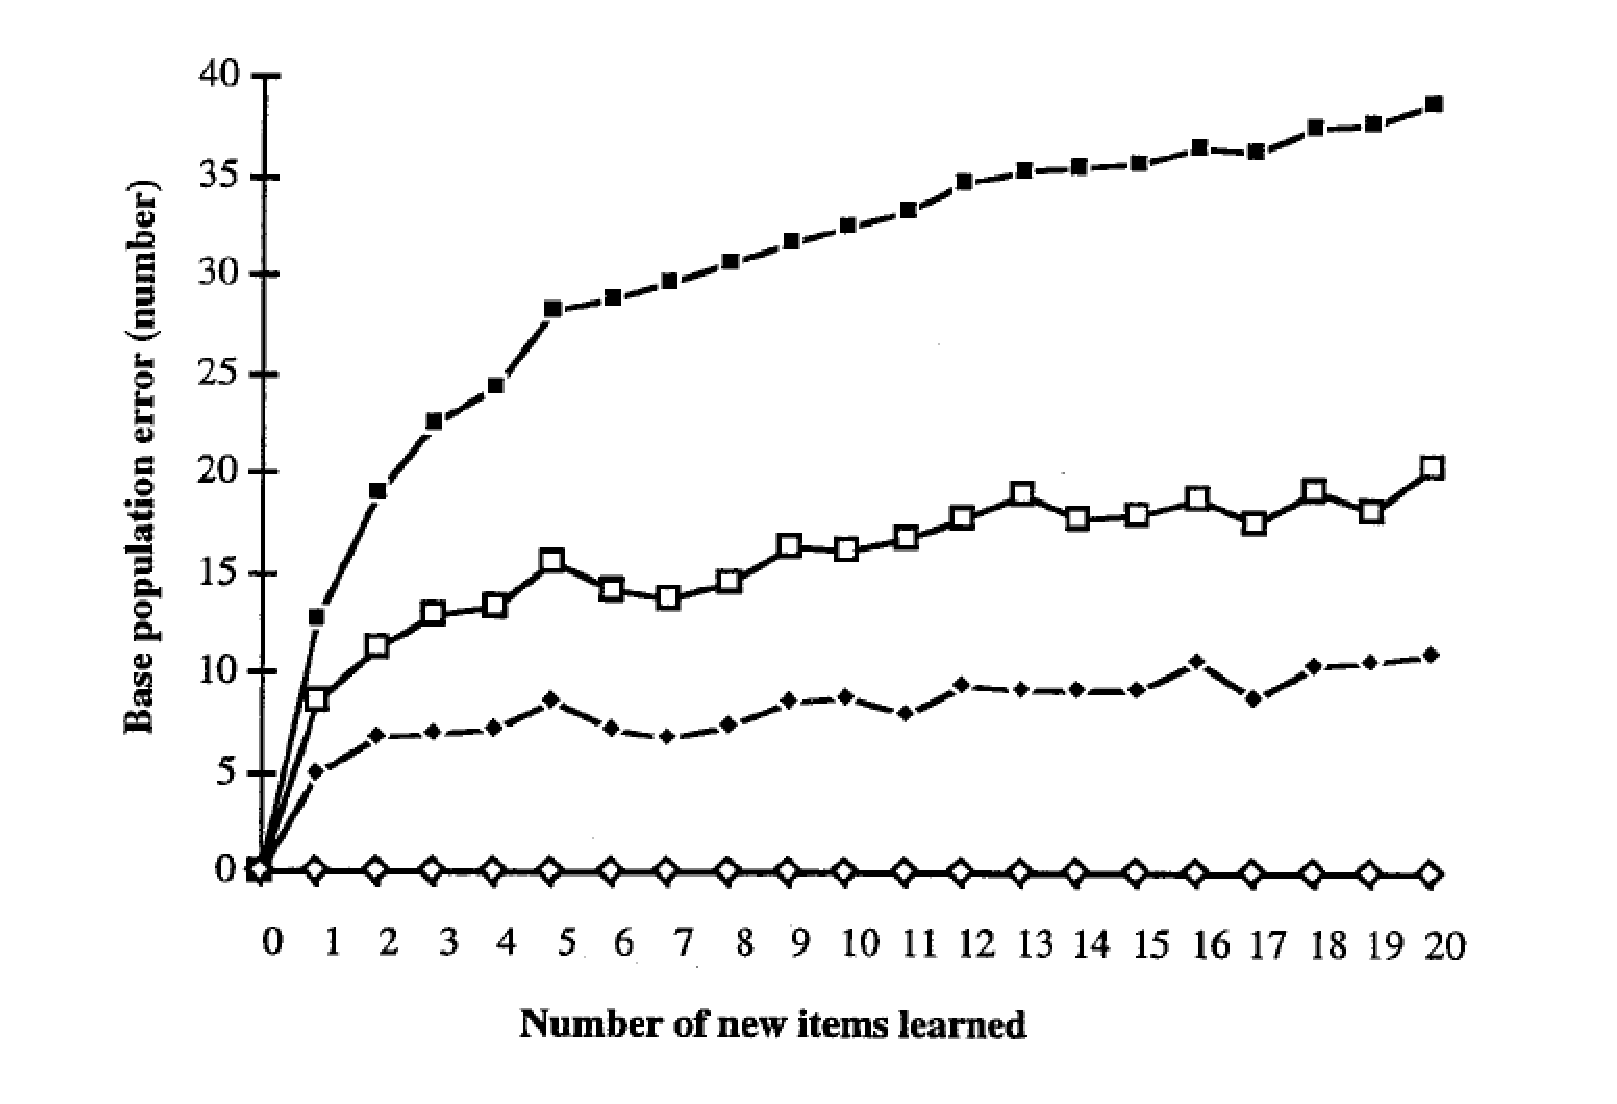
\includegraphics{Figures/HOP-CP.eps} %\input{Figures/HOP-CP} %
\clearpage
	% GNUPLOT: LaTeX picture with Postscript
\begingroup%
\makeatletter%
\newcommand{\GNUPLOTspecial}{%
  \@sanitize\catcode`\%=14\relax\special}%
\setlength{\unitlength}{0.0500bp}%
\begin{picture}(7200,5040)(0,0)%
  {\GNUPLOTspecial{"
%!PS-Adobe-2.0 EPSF-2.0
%%Title: WeightDecayHop.tex
%%Creator: gnuplot 4.2 patchlevel 2 
%%CreationDate: Thu Nov 01 12:30:50 2007
%%DocumentFonts: 
%%BoundingBox: 0 0 360 252
%%EndComments
%%BeginProlog
/gnudict 256 dict def
gnudict begin
%
% The following 6 true/false flags may be edited by hand if required
% The unit line width may also be changed
%
/Color true def
/Blacktext true def
/Solid false def
/Dashlength 1 def
/Landscape false def
/Level1 false def
/Rounded false def
/TransparentPatterns false def
/gnulinewidth 5.000 def
/userlinewidth gnulinewidth def
%
/vshift -66 def
/dl1 {
  10.0 Dashlength mul mul
  Rounded { currentlinewidth 0.75 mul sub dup 0 le { pop 0.01 } if } if
} def
/dl2 {
  10.0 Dashlength mul mul
  Rounded { currentlinewidth 0.75 mul add } if
} def
/hpt_ 31.5 def
/vpt_ 31.5 def
/hpt hpt_ def
/vpt vpt_ def
Level1 {} {
/SDict 10 dict def
systemdict /pdfmark known not {
  userdict /pdfmark systemdict /cleartomark get put
} if
SDict begin [
  /Title (WeightDecayHop.tex)
  /Subject (gnuplot plot)
  /Creator (gnuplot 4.2 patchlevel 2 )
  /Author (Simon)
%  /Producer (gnuplot)
%  /Keywords ()
  /CreationDate (Thu Nov 01 12:30:50 2007)
  /DOCINFO pdfmark
end
} ifelse
%
% Gnuplot Prolog Version 4.2 (August 2006)
%
/M {moveto} bind def
/L {lineto} bind def
/R {rmoveto} bind def
/V {rlineto} bind def
/N {newpath moveto} bind def
/Z {closepath} bind def
/C {setrgbcolor} bind def
/f {rlineto fill} bind def
/vpt2 vpt 2 mul def
/hpt2 hpt 2 mul def
/Lshow {currentpoint stroke M 0 vshift R 
	Blacktext {gsave 0 setgray show grestore} {show} ifelse} def
/Rshow {currentpoint stroke M dup stringwidth pop neg vshift R
	Blacktext {gsave 0 setgray show grestore} {show} ifelse} def
/Cshow {currentpoint stroke M dup stringwidth pop -2 div vshift R 
	Blacktext {gsave 0 setgray show grestore} {show} ifelse} def
/UP {dup vpt_ mul /vpt exch def hpt_ mul /hpt exch def
  /hpt2 hpt 2 mul def /vpt2 vpt 2 mul def} def
/DL {Color {setrgbcolor Solid {pop []} if 0 setdash}
 {pop pop pop 0 setgray Solid {pop []} if 0 setdash} ifelse} def
/BL {stroke userlinewidth 2 mul setlinewidth
	Rounded {1 setlinejoin 1 setlinecap} if} def
/AL {stroke userlinewidth 2 div setlinewidth
	Rounded {1 setlinejoin 1 setlinecap} if} def
/UL {dup gnulinewidth mul /userlinewidth exch def
	dup 1 lt {pop 1} if 10 mul /udl exch def} def
/PL {stroke userlinewidth setlinewidth
	Rounded {1 setlinejoin 1 setlinecap} if} def
% Default Line colors
/LCw {1 1 1} def
/LCb {0 0 0} def
/LCa {0 0 0} def
/LC0 {1 0 0} def
/LC1 {0 1 0} def
/LC2 {0 0 1} def
/LC3 {1 0 1} def
/LC4 {0 1 1} def
/LC5 {1 1 0} def
/LC6 {0 0 0} def
/LC7 {1 0.3 0} def
/LC8 {0.5 0.5 0.5} def
% Default Line Types
/LTw {PL [] 1 setgray} def
/LTb {BL [] LCb DL} def
/LTa {AL [1 udl mul 2 udl mul] 0 setdash LCa setrgbcolor} def
/LT0 {PL [] LC0 DL} def
/LT1 {PL [4 dl1 2 dl2] LC1 DL} def
/LT2 {PL [2 dl1 3 dl2] LC2 DL} def
/LT3 {PL [1 dl1 1.5 dl2] LC3 DL} def
/LT4 {PL [6 dl1 2 dl2 1 dl1 2 dl2] LC4 DL} def
/LT5 {PL [3 dl1 3 dl2 1 dl1 3 dl2] LC5 DL} def
/LT6 {PL [2 dl1 2 dl2 2 dl1 6 dl2] LC6 DL} def
/LT7 {PL [1 dl1 2 dl2 6 dl1 2 dl2 1 dl1 2 dl2] LC7 DL} def
/LT8 {PL [2 dl1 2 dl2 2 dl1 2 dl2 2 dl1 2 dl2 2 dl1 4 dl2] LC8 DL} def
/Pnt {stroke [] 0 setdash gsave 1 setlinecap M 0 0 V stroke grestore} def
/Dia {stroke [] 0 setdash 2 copy vpt add M
  hpt neg vpt neg V hpt vpt neg V
  hpt vpt V hpt neg vpt V closepath stroke
  Pnt} def
/Pls {stroke [] 0 setdash vpt sub M 0 vpt2 V
  currentpoint stroke M
  hpt neg vpt neg R hpt2 0 V stroke
 } def
/Box {stroke [] 0 setdash 2 copy exch hpt sub exch vpt add M
  0 vpt2 neg V hpt2 0 V 0 vpt2 V
  hpt2 neg 0 V closepath stroke
  Pnt} def
/Crs {stroke [] 0 setdash exch hpt sub exch vpt add M
  hpt2 vpt2 neg V currentpoint stroke M
  hpt2 neg 0 R hpt2 vpt2 V stroke} def
/TriU {stroke [] 0 setdash 2 copy vpt 1.12 mul add M
  hpt neg vpt -1.62 mul V
  hpt 2 mul 0 V
  hpt neg vpt 1.62 mul V closepath stroke
  Pnt} def
/Star {2 copy Pls Crs} def
/BoxF {stroke [] 0 setdash exch hpt sub exch vpt add M
  0 vpt2 neg V hpt2 0 V 0 vpt2 V
  hpt2 neg 0 V closepath fill} def
/TriUF {stroke [] 0 setdash vpt 1.12 mul add M
  hpt neg vpt -1.62 mul V
  hpt 2 mul 0 V
  hpt neg vpt 1.62 mul V closepath fill} def
/TriD {stroke [] 0 setdash 2 copy vpt 1.12 mul sub M
  hpt neg vpt 1.62 mul V
  hpt 2 mul 0 V
  hpt neg vpt -1.62 mul V closepath stroke
  Pnt} def
/TriDF {stroke [] 0 setdash vpt 1.12 mul sub M
  hpt neg vpt 1.62 mul V
  hpt 2 mul 0 V
  hpt neg vpt -1.62 mul V closepath fill} def
/DiaF {stroke [] 0 setdash vpt add M
  hpt neg vpt neg V hpt vpt neg V
  hpt vpt V hpt neg vpt V closepath fill} def
/Pent {stroke [] 0 setdash 2 copy gsave
  translate 0 hpt M 4 {72 rotate 0 hpt L} repeat
  closepath stroke grestore Pnt} def
/PentF {stroke [] 0 setdash gsave
  translate 0 hpt M 4 {72 rotate 0 hpt L} repeat
  closepath fill grestore} def
/Circle {stroke [] 0 setdash 2 copy
  hpt 0 360 arc stroke Pnt} def
/CircleF {stroke [] 0 setdash hpt 0 360 arc fill} def
/C0 {BL [] 0 setdash 2 copy moveto vpt 90 450 arc} bind def
/C1 {BL [] 0 setdash 2 copy moveto
	2 copy vpt 0 90 arc closepath fill
	vpt 0 360 arc closepath} bind def
/C2 {BL [] 0 setdash 2 copy moveto
	2 copy vpt 90 180 arc closepath fill
	vpt 0 360 arc closepath} bind def
/C3 {BL [] 0 setdash 2 copy moveto
	2 copy vpt 0 180 arc closepath fill
	vpt 0 360 arc closepath} bind def
/C4 {BL [] 0 setdash 2 copy moveto
	2 copy vpt 180 270 arc closepath fill
	vpt 0 360 arc closepath} bind def
/C5 {BL [] 0 setdash 2 copy moveto
	2 copy vpt 0 90 arc
	2 copy moveto
	2 copy vpt 180 270 arc closepath fill
	vpt 0 360 arc} bind def
/C6 {BL [] 0 setdash 2 copy moveto
	2 copy vpt 90 270 arc closepath fill
	vpt 0 360 arc closepath} bind def
/C7 {BL [] 0 setdash 2 copy moveto
	2 copy vpt 0 270 arc closepath fill
	vpt 0 360 arc closepath} bind def
/C8 {BL [] 0 setdash 2 copy moveto
	2 copy vpt 270 360 arc closepath fill
	vpt 0 360 arc closepath} bind def
/C9 {BL [] 0 setdash 2 copy moveto
	2 copy vpt 270 450 arc closepath fill
	vpt 0 360 arc closepath} bind def
/C10 {BL [] 0 setdash 2 copy 2 copy moveto vpt 270 360 arc closepath fill
	2 copy moveto
	2 copy vpt 90 180 arc closepath fill
	vpt 0 360 arc closepath} bind def
/C11 {BL [] 0 setdash 2 copy moveto
	2 copy vpt 0 180 arc closepath fill
	2 copy moveto
	2 copy vpt 270 360 arc closepath fill
	vpt 0 360 arc closepath} bind def
/C12 {BL [] 0 setdash 2 copy moveto
	2 copy vpt 180 360 arc closepath fill
	vpt 0 360 arc closepath} bind def
/C13 {BL [] 0 setdash 2 copy moveto
	2 copy vpt 0 90 arc closepath fill
	2 copy moveto
	2 copy vpt 180 360 arc closepath fill
	vpt 0 360 arc closepath} bind def
/C14 {BL [] 0 setdash 2 copy moveto
	2 copy vpt 90 360 arc closepath fill
	vpt 0 360 arc} bind def
/C15 {BL [] 0 setdash 2 copy vpt 0 360 arc closepath fill
	vpt 0 360 arc closepath} bind def
/Rec {newpath 4 2 roll moveto 1 index 0 rlineto 0 exch rlineto
	neg 0 rlineto closepath} bind def
/Square {dup Rec} bind def
/Bsquare {vpt sub exch vpt sub exch vpt2 Square} bind def
/S0 {BL [] 0 setdash 2 copy moveto 0 vpt rlineto BL Bsquare} bind def
/S1 {BL [] 0 setdash 2 copy vpt Square fill Bsquare} bind def
/S2 {BL [] 0 setdash 2 copy exch vpt sub exch vpt Square fill Bsquare} bind def
/S3 {BL [] 0 setdash 2 copy exch vpt sub exch vpt2 vpt Rec fill Bsquare} bind def
/S4 {BL [] 0 setdash 2 copy exch vpt sub exch vpt sub vpt Square fill Bsquare} bind def
/S5 {BL [] 0 setdash 2 copy 2 copy vpt Square fill
	exch vpt sub exch vpt sub vpt Square fill Bsquare} bind def
/S6 {BL [] 0 setdash 2 copy exch vpt sub exch vpt sub vpt vpt2 Rec fill Bsquare} bind def
/S7 {BL [] 0 setdash 2 copy exch vpt sub exch vpt sub vpt vpt2 Rec fill
	2 copy vpt Square fill Bsquare} bind def
/S8 {BL [] 0 setdash 2 copy vpt sub vpt Square fill Bsquare} bind def
/S9 {BL [] 0 setdash 2 copy vpt sub vpt vpt2 Rec fill Bsquare} bind def
/S10 {BL [] 0 setdash 2 copy vpt sub vpt Square fill 2 copy exch vpt sub exch vpt Square fill
	Bsquare} bind def
/S11 {BL [] 0 setdash 2 copy vpt sub vpt Square fill 2 copy exch vpt sub exch vpt2 vpt Rec fill
	Bsquare} bind def
/S12 {BL [] 0 setdash 2 copy exch vpt sub exch vpt sub vpt2 vpt Rec fill Bsquare} bind def
/S13 {BL [] 0 setdash 2 copy exch vpt sub exch vpt sub vpt2 vpt Rec fill
	2 copy vpt Square fill Bsquare} bind def
/S14 {BL [] 0 setdash 2 copy exch vpt sub exch vpt sub vpt2 vpt Rec fill
	2 copy exch vpt sub exch vpt Square fill Bsquare} bind def
/S15 {BL [] 0 setdash 2 copy Bsquare fill Bsquare} bind def
/D0 {gsave translate 45 rotate 0 0 S0 stroke grestore} bind def
/D1 {gsave translate 45 rotate 0 0 S1 stroke grestore} bind def
/D2 {gsave translate 45 rotate 0 0 S2 stroke grestore} bind def
/D3 {gsave translate 45 rotate 0 0 S3 stroke grestore} bind def
/D4 {gsave translate 45 rotate 0 0 S4 stroke grestore} bind def
/D5 {gsave translate 45 rotate 0 0 S5 stroke grestore} bind def
/D6 {gsave translate 45 rotate 0 0 S6 stroke grestore} bind def
/D7 {gsave translate 45 rotate 0 0 S7 stroke grestore} bind def
/D8 {gsave translate 45 rotate 0 0 S8 stroke grestore} bind def
/D9 {gsave translate 45 rotate 0 0 S9 stroke grestore} bind def
/D10 {gsave translate 45 rotate 0 0 S10 stroke grestore} bind def
/D11 {gsave translate 45 rotate 0 0 S11 stroke grestore} bind def
/D12 {gsave translate 45 rotate 0 0 S12 stroke grestore} bind def
/D13 {gsave translate 45 rotate 0 0 S13 stroke grestore} bind def
/D14 {gsave translate 45 rotate 0 0 S14 stroke grestore} bind def
/D15 {gsave translate 45 rotate 0 0 S15 stroke grestore} bind def
/DiaE {stroke [] 0 setdash vpt add M
  hpt neg vpt neg V hpt vpt neg V
  hpt vpt V hpt neg vpt V closepath stroke} def
/BoxE {stroke [] 0 setdash exch hpt sub exch vpt add M
  0 vpt2 neg V hpt2 0 V 0 vpt2 V
  hpt2 neg 0 V closepath stroke} def
/TriUE {stroke [] 0 setdash vpt 1.12 mul add M
  hpt neg vpt -1.62 mul V
  hpt 2 mul 0 V
  hpt neg vpt 1.62 mul V closepath stroke} def
/TriDE {stroke [] 0 setdash vpt 1.12 mul sub M
  hpt neg vpt 1.62 mul V
  hpt 2 mul 0 V
  hpt neg vpt -1.62 mul V closepath stroke} def
/PentE {stroke [] 0 setdash gsave
  translate 0 hpt M 4 {72 rotate 0 hpt L} repeat
  closepath stroke grestore} def
/CircE {stroke [] 0 setdash 
  hpt 0 360 arc stroke} def
/Opaque {gsave closepath 1 setgray fill grestore 0 setgray closepath} def
/DiaW {stroke [] 0 setdash vpt add M
  hpt neg vpt neg V hpt vpt neg V
  hpt vpt V hpt neg vpt V Opaque stroke} def
/BoxW {stroke [] 0 setdash exch hpt sub exch vpt add M
  0 vpt2 neg V hpt2 0 V 0 vpt2 V
  hpt2 neg 0 V Opaque stroke} def
/TriUW {stroke [] 0 setdash vpt 1.12 mul add M
  hpt neg vpt -1.62 mul V
  hpt 2 mul 0 V
  hpt neg vpt 1.62 mul V Opaque stroke} def
/TriDW {stroke [] 0 setdash vpt 1.12 mul sub M
  hpt neg vpt 1.62 mul V
  hpt 2 mul 0 V
  hpt neg vpt -1.62 mul V Opaque stroke} def
/PentW {stroke [] 0 setdash gsave
  translate 0 hpt M 4 {72 rotate 0 hpt L} repeat
  Opaque stroke grestore} def
/CircW {stroke [] 0 setdash 
  hpt 0 360 arc Opaque stroke} def
/BoxFill {gsave Rec 1 setgray fill grestore} def
/Density {
  /Fillden exch def
  currentrgbcolor
  /ColB exch def /ColG exch def /ColR exch def
  /ColR ColR Fillden mul Fillden sub 1 add def
  /ColG ColG Fillden mul Fillden sub 1 add def
  /ColB ColB Fillden mul Fillden sub 1 add def
  ColR ColG ColB setrgbcolor} def
/BoxColFill {gsave Rec PolyFill} def
/PolyFill {gsave Density fill grestore grestore} def
/h {rlineto rlineto rlineto gsave fill grestore} bind def
%
% PostScript Level 1 Pattern Fill routine for rectangles
% Usage: x y w h s a XX PatternFill
%	x,y = lower left corner of box to be filled
%	w,h = width and height of box
%	  a = angle in degrees between lines and x-axis
%	 XX = 0/1 for no/yes cross-hatch
%
/PatternFill {gsave /PFa [ 9 2 roll ] def
  PFa 0 get PFa 2 get 2 div add PFa 1 get PFa 3 get 2 div add translate
  PFa 2 get -2 div PFa 3 get -2 div PFa 2 get PFa 3 get Rec
  gsave 1 setgray fill grestore clip
  currentlinewidth 0.5 mul setlinewidth
  /PFs PFa 2 get dup mul PFa 3 get dup mul add sqrt def
  0 0 M PFa 5 get rotate PFs -2 div dup translate
  0 1 PFs PFa 4 get div 1 add floor cvi
	{PFa 4 get mul 0 M 0 PFs V} for
  0 PFa 6 get ne {
	0 1 PFs PFa 4 get div 1 add floor cvi
	{PFa 4 get mul 0 2 1 roll M PFs 0 V} for
 } if
  stroke grestore} def
%
/languagelevel where
 {pop languagelevel} {1} ifelse
 2 lt
	{/InterpretLevel1 true def}
	{/InterpretLevel1 Level1 def}
 ifelse
%
% PostScript level 2 pattern fill definitions
%
/Level2PatternFill {
/Tile8x8 {/PaintType 2 /PatternType 1 /TilingType 1 /BBox [0 0 8 8] /XStep 8 /YStep 8}
	bind def
/KeepColor {currentrgbcolor [/Pattern /DeviceRGB] setcolorspace} bind def
<< Tile8x8
 /PaintProc {0.5 setlinewidth pop 0 0 M 8 8 L 0 8 M 8 0 L stroke} 
>> matrix makepattern
/Pat1 exch def
<< Tile8x8
 /PaintProc {0.5 setlinewidth pop 0 0 M 8 8 L 0 8 M 8 0 L stroke
	0 4 M 4 8 L 8 4 L 4 0 L 0 4 L stroke}
>> matrix makepattern
/Pat2 exch def
<< Tile8x8
 /PaintProc {0.5 setlinewidth pop 0 0 M 0 8 L
	8 8 L 8 0 L 0 0 L fill}
>> matrix makepattern
/Pat3 exch def
<< Tile8x8
 /PaintProc {0.5 setlinewidth pop -4 8 M 8 -4 L
	0 12 M 12 0 L stroke}
>> matrix makepattern
/Pat4 exch def
<< Tile8x8
 /PaintProc {0.5 setlinewidth pop -4 0 M 8 12 L
	0 -4 M 12 8 L stroke}
>> matrix makepattern
/Pat5 exch def
<< Tile8x8
 /PaintProc {0.5 setlinewidth pop -2 8 M 4 -4 L
	0 12 M 8 -4 L 4 12 M 10 0 L stroke}
>> matrix makepattern
/Pat6 exch def
<< Tile8x8
 /PaintProc {0.5 setlinewidth pop -2 0 M 4 12 L
	0 -4 M 8 12 L 4 -4 M 10 8 L stroke}
>> matrix makepattern
/Pat7 exch def
<< Tile8x8
 /PaintProc {0.5 setlinewidth pop 8 -2 M -4 4 L
	12 0 M -4 8 L 12 4 M 0 10 L stroke}
>> matrix makepattern
/Pat8 exch def
<< Tile8x8
 /PaintProc {0.5 setlinewidth pop 0 -2 M 12 4 L
	-4 0 M 12 8 L -4 4 M 8 10 L stroke}
>> matrix makepattern
/Pat9 exch def
/Pattern1 {PatternBgnd KeepColor Pat1 setpattern} bind def
/Pattern2 {PatternBgnd KeepColor Pat2 setpattern} bind def
/Pattern3 {PatternBgnd KeepColor Pat3 setpattern} bind def
/Pattern4 {PatternBgnd KeepColor Landscape {Pat5} {Pat4} ifelse setpattern} bind def
/Pattern5 {PatternBgnd KeepColor Landscape {Pat4} {Pat5} ifelse setpattern} bind def
/Pattern6 {PatternBgnd KeepColor Landscape {Pat9} {Pat6} ifelse setpattern} bind def
/Pattern7 {PatternBgnd KeepColor Landscape {Pat8} {Pat7} ifelse setpattern} bind def
} def
%
%
%End of PostScript Level 2 code
%
/PatternBgnd {
  TransparentPatterns {} {gsave 1 setgray fill grestore} ifelse
} def
%
% Substitute for Level 2 pattern fill codes with
% grayscale if Level 2 support is not selected.
%
/Level1PatternFill {
/Pattern1 {0.250 Density} bind def
/Pattern2 {0.500 Density} bind def
/Pattern3 {0.750 Density} bind def
/Pattern4 {0.125 Density} bind def
/Pattern5 {0.375 Density} bind def
/Pattern6 {0.625 Density} bind def
/Pattern7 {0.875 Density} bind def
} def
%
% Now test for support of Level 2 code
%
Level1 {Level1PatternFill} {Level2PatternFill} ifelse
%
/Symbol-Oblique /Symbol findfont [1 0 .167 1 0 0] makefont
dup length dict begin {1 index /FID eq {pop pop} {def} ifelse} forall
currentdict end definefont pop
end
%%EndProlog
gnudict begin
gsave
0 0 translate
0.050 0.050 scale
0 setgray
newpath
gsave % colour palette begin
/maxcolors 0 def
/HSV2RGB {  exch dup 0.0 eq {pop exch pop dup dup} % achromatic gray
  { /HSVs exch def /HSVv exch def 6.0 mul dup floor dup 3 1 roll sub
     /HSVf exch def /HSVi exch cvi def /HSVp HSVv 1.0 HSVs sub mul def
	 /HSVq HSVv 1.0 HSVs HSVf mul sub mul def 
	 /HSVt HSVv 1.0 HSVs 1.0 HSVf sub mul sub mul def
	 /HSVi HSVi 6 mod def 0 HSVi eq {HSVv HSVt HSVp}
	 {1 HSVi eq {HSVq HSVv HSVp}{2 HSVi eq {HSVp HSVv HSVt}
	 {3 HSVi eq {HSVp HSVq HSVv}{4 HSVi eq {HSVt HSVp HSVv}
	 {HSVv HSVp HSVq} ifelse} ifelse} ifelse} ifelse} ifelse
  } ifelse} def
/Constrain {
  dup 0 lt {0 exch pop}{dup 1 gt {1 exch pop} if} ifelse} def
/YIQ2RGB {
  3 copy -1.702 mul exch -1.105 mul add add Constrain 4 1 roll
  3 copy -0.647 mul exch -0.272 mul add add Constrain 5 1 roll
  0.621 mul exch -0.956 mul add add Constrain 3 1 roll } def
/CMY2RGB {  1 exch sub exch 1 exch sub 3 2 roll 1 exch sub 3 1 roll exch } def
/XYZ2RGB {  3 copy -0.9017 mul exch -0.1187 mul add exch 0.0585 mul exch add
  Constrain 4 1 roll 3 copy -0.0279 mul exch 1.999 mul add exch
  -0.9844 mul add Constrain 5 1 roll -0.2891 mul exch -0.5338 mul add
  exch 1.91 mul exch add Constrain 3 1 roll} def
/SelectSpace {ColorSpace (HSV) eq {HSV2RGB}{ColorSpace (XYZ) eq {
  XYZ2RGB}{ColorSpace (CMY) eq {CMY2RGB}{ColorSpace (YIQ) eq {YIQ2RGB}
  if} ifelse} ifelse} ifelse} def
/InterpolatedColor false def
/cF7 {sqrt} bind def	% sqrt(x)
/cF5 {dup dup mul mul} bind def	% x^3
/cF15 {360 mul sin} bind def	% sin(360x)
/pm3dround {maxcolors 0 gt {dup 1 ge
	{pop 1} {maxcolors mul floor maxcolors 1 sub div} ifelse} if} def
/pm3dGamma 1.0 1.5 div def
/ColorSpace (RGB) def
Color true and { % COLOUR vs. GRAY map
  InterpolatedColor { %% Interpolation vs. RGB-Formula
    /g {stroke pm3dround /grayv exch def interpolate
        SelectSpace setrgbcolor} bind def
  }{
  /g {stroke pm3dround dup cF7 Constrain exch dup cF5 Constrain exch cF15 Constrain 
       SelectSpace setrgbcolor} bind def
  } ifelse
}{
  /g {stroke pm3dround pm3dGamma exp setgray} bind def
} ifelse
1.000 UL
LTb
1083 663 M
-63 0 V
63 591 R
-63 0 V
63 591 R
-63 0 V
63 591 R
-63 0 V
63 591 R
-63 0 V
63 591 R
-63 0 V
63 591 R
-63 0 V
63 591 R
-63 0 V
1083 663 M
0 -63 V
615 63 R
0 -63 V
614 63 R
0 -63 V
615 63 R
0 -63 V
614 63 R
0 -63 V
615 63 R
0 -63 V
614 63 R
0 -63 V
615 63 R
0 -63 V
615 63 R
0 -63 V
614 63 R
0 -63 V
1083 4800 M
0 -4137 V
5777 0 V
0 4137 V
-5777 0 V
stroke
LCb setrgbcolor
LTb
LCb setrgbcolor
LTb
1.000 UP
1.000 UL
LTb
0.000 UP
0.500 UL
LT1
1.00 0.53 0.53 C 1083 1550 M
-7 0 R
13 0 V
-13 0 R
13 0 V
117 295 R
-7 0 R
13 0 V
-13 0 R
13 0 V
117 296 R
-7 0 R
13 0 V
-13 0 R
13 0 V
117 295 R
-7 0 R
13 0 V
-13 0 R
13 0 V
117 296 R
-7 0 R
13 0 V
-13 0 R
13 0 V
117 254 R
0 82 V
-7 -82 R
13 0 V
-13 82 R
13 0 V
116 28 R
0 335 V
-7 -335 R
13 0 V
-13 335 R
13 0 V
117 -126 R
0 390 V
-7 -390 R
13 0 V
-13 390 R
13 0 V
117 -360 R
0 626 V
-7 -626 R
13 0 V
-13 626 R
13 0 V
117 -457 R
0 642 V
-7 -642 R
13 0 V
-13 642 R
13 0 V
117 -707 R
0 890 V
-7 -890 R
13 0 V
-13 890 R
13 0 V
117 -898 R
0 1083 V
-7 -1083 R
13 0 V
-13 1083 R
13 0 V
2558 3189 M
0 1331 V
-7 -1331 R
13 0 V
-13 1331 R
13 0 V
2681 3024 M
0 1543 V
-7 -1543 R
13 0 V
-13 1543 R
13 0 V
2804 2735 M
0 1588 V
-7 -1588 R
13 0 V
-13 1588 R
13 0 V
2927 2651 M
0 1580 V
-7 -1580 R
13 0 V
-13 1580 R
13 0 V
3050 2299 M
0 1515 V
-7 -1515 R
13 0 V
-13 1515 R
13 0 V
3173 2234 M
0 1408 V
-7 -1408 R
13 0 V
-13 1408 R
13 0 V
3295 1880 M
0 1467 V
-7 -1467 R
3301 1880 L
-13 1467 R
13 0 V
3418 1799 M
0 1333 V
-7 -1333 R
13 0 V
-13 1333 R
13 0 V
3541 1400 M
0 1245 V
-7 -1245 R
13 0 V
-13 1245 R
13 0 V
3664 1190 M
0 1428 V
-7 -1428 R
13 0 V
-13 1428 R
13 0 V
3787 1028 M
0 1161 V
-7 -1161 R
13 0 V
-13 1161 R
13 0 V
3910 984 M
0 1131 V
3903 984 M
13 0 V
-13 1131 R
13 0 V
4033 861 M
0 963 V
-7 -963 R
13 0 V
-13 963 R
13 0 V
4156 874 M
0 819 V
-7 -819 R
13 0 V
-13 819 R
13 0 V
4279 743 M
0 726 V
-7 -726 R
13 0 V
-13 726 R
13 0 V
4402 742 M
0 670 V
-7 -670 R
13 0 V
-13 670 R
13 0 V
4525 663 M
0 592 V
-7 -592 R
13 0 V
-13 592 R
13 0 V
4648 663 M
0 565 V
-7 -565 R
13 0 V
-13 565 R
13 0 V
4770 663 M
0 455 V
-7 -455 R
13 0 V
-13 455 R
13 0 V
4893 663 M
0 363 V
-7 -363 R
13 0 V
-13 363 R
13 0 V
5016 663 M
0 247 V
-7 -247 R
13 0 V
-13 247 R
13 0 V
5139 663 M
0 248 V
-7 -248 R
13 0 V
-13 248 R
13 0 V
5262 663 M
0 135 V
-7 -135 R
13 0 V
-13 135 R
13 0 V
5385 663 M
0 143 V
-7 -143 R
13 0 V
-13 143 R
13 0 V
5508 663 M
5508 777 L
-7 -114 R
13 0 V
-13 114 R
13 0 V
5631 663 M
0 110 V
-7 -110 R
13 0 V
-13 110 R
13 0 V
5754 663 M
0 29 V
-7 -29 R
13 0 V
-13 29 R
13 0 V
117 -29 R
0 50 V
-7 -50 R
13 0 V
-13 50 R
13 0 V
117 -50 R
0 41 V
-7 -41 R
13 0 V
-13 41 R
13 0 V
117 -41 R
0 29 V
-7 -29 R
13 0 V
-13 29 R
13 0 V
116 -29 R
0 50 V
-7 -50 R
13 0 V
-13 50 R
13 0 V
117 -50 R
0 41 V
-7 -41 R
13 0 V
-13 41 R
13 0 V
117 -41 R
-7 0 R
13 0 V
-13 0 R
13 0 V
117 0 R
-7 0 R
13 0 V
-13 0 R
13 0 V
117 0 R
-7 0 R
13 0 V
-13 0 R
13 0 V
117 0 R
0 29 V
-7 -29 R
13 0 V
-13 29 R
13 0 V
1083 1550 Star
1206 1845 Star
1329 2141 Star
1452 2436 Star
1575 2732 Star
1698 3027 Star
1820 3263 Star
1943 3500 Star
2066 3648 Star
2189 3825 Star
2312 3884 Star
2435 3973 Star
2558 3854 Star
2681 3795 Star
2804 3529 Star
2927 3441 Star
3050 3057 Star
3173 2938 Star
3295 2613 Star
3418 2466 Star
3541 2022 Star
3664 1904 Star
3787 1609 Star
3910 1550 Star
4033 1343 Star
4156 1284 Star
4279 1106 Star
4402 1077 Star
4525 959 Star
4648 929 Star
4770 870 Star
4893 811 Star
5016 752 Star
5139 752 Star
5262 693 Star
5385 693 Star
5508 693 Star
5631 693 Star
5754 663 Star
5877 663 Star
6000 663 Star
6123 663 Star
6245 663 Star
6368 663 Star
6491 663 Star
6614 663 Star
6737 663 Star
6860 663 Star
1.000 UL
LT0
0.60 0.00 0.00 C LTb
LT0
0.60 0.00 0.00 C 6077 4612 M
543 0 V
1083 1550 M
123 295 V
123 296 V
123 295 V
123 296 V
123 295 V
122 236 V
123 237 V
123 148 V
123 177 V
123 59 V
123 89 V
123 -119 V
123 -59 V
123 -266 V
123 -88 V
123 -384 V
123 -119 V
122 -325 V
123 -147 V
123 -444 V
123 -118 V
123 -295 V
123 -59 V
123 -207 V
123 -59 V
123 -178 V
123 -29 V
4525 959 L
123 -30 V
122 -59 V
123 -59 V
123 -59 V
123 0 V
123 -59 V
123 0 V
123 0 V
123 0 V
123 -30 V
123 0 V
123 0 V
123 0 V
122 0 V
123 0 V
123 0 V
123 0 V
123 0 V
123 0 V
0.000 UP
stroke
0.500 UL
LT1
0.53 0.53 0.53 C 1083 1550 M
-7 0 R
13 0 V
-13 0 R
13 0 V
117 295 R
-7 0 R
13 0 V
-13 0 R
13 0 V
117 296 R
-7 0 R
13 0 V
-13 0 R
13 0 V
117 203 R
0 154 V
-7 -154 R
13 0 V
-13 154 R
13 0 V
117 17 R
0 291 V
-7 -291 R
13 0 V
-13 291 R
13 0 V
117 -217 R
0 451 V
-7 -451 R
13 0 V
-13 451 R
13 0 V
116 -451 R
0 551 V
-7 -551 R
13 0 V
-13 551 R
13 0 V
117 -536 R
0 592 V
-7 -592 R
13 0 V
-13 592 R
13 0 V
117 -645 R
0 603 V
-7 -603 R
13 0 V
-13 603 R
13 0 V
117 -649 R
0 583 V
-7 -583 R
13 0 V
-13 583 R
13 0 V
117 -574 R
0 565 V
-7 -565 R
13 0 V
-13 565 R
13 0 V
117 -571 R
0 601 V
-7 -601 R
13 0 V
-13 601 R
13 0 V
117 -656 R
0 627 V
-7 -627 R
13 0 V
-13 627 R
13 0 V
117 -626 R
0 620 V
-7 -620 R
13 0 V
-13 620 R
13 0 V
117 -636 R
0 582 V
-7 -582 R
13 0 V
-13 582 R
13 0 V
117 -634 R
0 637 V
-7 -637 R
13 0 V
-13 637 R
13 0 V
117 -715 R
0 658 V
-7 -658 R
13 0 V
-13 658 R
13 0 V
117 -618 R
0 660 V
-7 -660 R
13 0 V
-13 660 R
13 0 V
116 -612 R
3295 3020 L
-7 -624 R
13 0 V
-13 624 R
13 0 V
117 -637 R
0 614 V
-7 -614 R
13 0 V
-13 614 R
13 0 V
117 -597 R
0 609 V
-7 -609 R
13 0 V
-13 609 R
13 0 V
117 -628 R
0 671 V
-7 -671 R
13 0 V
-13 671 R
13 0 V
117 -679 R
0 664 V
-7 -664 R
13 0 V
-13 664 R
13 0 V
117 -610 R
0 597 V
-7 -597 R
13 0 V
-13 597 R
13 0 V
117 -625 R
0 571 V
-7 -571 R
13 0 V
-13 571 R
13 0 V
117 -511 R
0 575 V
-7 -575 R
13 0 V
-13 575 R
13 0 V
117 -634 R
0 621 V
-7 -621 R
13 0 V
-13 621 R
13 0 V
117 -660 R
0 611 V
-7 -611 R
13 0 V
-13 611 R
13 0 V
117 -652 R
0 640 V
-7 -640 R
13 0 V
-13 640 R
13 0 V
117 -629 R
0 641 V
-7 -641 R
13 0 V
-13 641 R
13 0 V
116 -631 R
0 651 V
-7 -651 R
13 0 V
-13 651 R
13 0 V
117 -667 R
0 682 V
-7 -682 R
13 0 V
-13 682 R
13 0 V
117 -696 R
0 652 V
-7 -652 R
13 0 V
-13 652 R
13 0 V
117 -624 R
0 708 V
-7 -708 R
13 0 V
-13 708 R
13 0 V
117 -748 R
0 664 V
-7 -664 R
13 0 V
-13 664 R
13 0 V
117 -616 R
0 603 V
-7 -603 R
13 0 V
-13 603 R
5391 2950 L
117 -627 R
0 687 V
-7 -687 R
13 0 V
-13 687 R
13 0 V
117 -617 R
0 641 V
-7 -641 R
13 0 V
-13 641 R
13 0 V
117 -619 R
0 592 V
-7 -592 R
13 0 V
-13 592 R
13 0 V
117 -576 R
0 566 V
-7 -566 R
13 0 V
-13 566 R
13 0 V
117 -572 R
0 625 V
-7 -625 R
13 0 V
-13 625 R
13 0 V
117 -666 R
0 618 V
-7 -618 R
13 0 V
-13 618 R
13 0 V
116 -636 R
0 690 V
-7 -690 R
13 0 V
-13 690 R
13 0 V
117 -702 R
0 619 V
-7 -619 R
13 0 V
-13 619 R
13 0 V
117 -565 R
0 683 V
-7 -683 R
13 0 V
-13 683 R
13 0 V
117 -732 R
0 639 V
-7 -639 R
13 0 V
-13 639 R
13 0 V
117 -618 R
0 585 V
-7 -585 R
13 0 V
-13 585 R
13 0 V
117 -589 R
0 622 V
-7 -622 R
13 0 V
-13 622 R
13 0 V
1083 1550 Pls
1206 1845 Pls
1329 2141 Pls
1452 2421 Pls
1575 2661 Pls
1698 2814 Pls
1820 2864 Pls
1943 2900 Pls
2066 2853 Pls
2189 2797 Pls
2312 2797 Pls
2435 2808 Pls
2558 2767 Pls
2681 2764 Pls
2804 2729 Pls
2927 2705 Pls
3050 2637 Pls
3173 2678 Pls
3295 2708 Pls
3418 2690 Pls
3541 2705 Pls
3664 2717 Pls
3787 2705 Pls
3910 2726 Pls
4033 2684 Pls
4156 2746 Pls
4279 2711 Pls
4402 2666 Pls
4525 2640 Pls
4648 2652 Pls
4770 2666 Pls
4893 2666 Pls
5016 2637 Pls
5139 2693 Pls
5262 2631 Pls
5385 2649 Pls
5508 2666 Pls
5631 2714 Pls
5754 2711 Pls
5877 2714 Pls
6000 2737 Pls
6123 2693 Pls
6245 2711 Pls
6368 2664 Pls
6491 2749 Pls
6614 2678 Pls
6737 2672 Pls
6860 2687 Pls
1.000 UL
LT1
0.00 0.00 0.00 C LTb
LT1
0.00 0.00 0.00 C 6077 4362 M
543 0 V
1083 1550 M
123 295 V
123 296 V
123 280 V
123 240 V
123 153 V
122 50 V
123 36 V
123 -47 V
123 -56 V
123 0 V
123 11 V
123 -41 V
123 -3 V
123 -35 V
123 -24 V
123 -68 V
123 41 V
122 30 V
123 -18 V
123 15 V
123 12 V
123 -12 V
123 21 V
123 -42 V
123 62 V
123 -35 V
123 -45 V
123 -26 V
123 12 V
122 14 V
123 0 V
123 -29 V
123 56 V
123 -62 V
123 18 V
123 17 V
123 48 V
123 -3 V
123 3 V
123 23 V
123 -44 V
122 18 V
123 -47 V
123 85 V
123 -71 V
123 -6 V
123 15 V
stroke
LTb
1083 4800 M
0 -4137 V
5777 0 V
0 4137 V
-5777 0 V
1.000 UP
stroke
grestore
end
showpage
  }}%
  \put(5957,4362){\makebox(0,0)[r]{\strut{}Weight Decay}}%
  \put(5957,4612){\makebox(0,0)[r]{\strut{}No Decay}}%
  \put(3971,100){\makebox(0,0){\strut{}Patterns Learnt}}%
  \put(200,2731){%
  \special{ps: gsave currentpoint currentpoint translate
270 rotate neg exch neg exch translate}%
  \makebox(0,0){\strut{}Number Stable}%
  \special{ps: currentpoint grestore moveto}%
  }%
  \put(6614,400){\makebox(0,0){\strut{}$48$}}%
  \put(6000,400){\makebox(0,0){\strut{}$43$}}%
  \put(5385,400){\makebox(0,0){\strut{}$38$}}%
  \put(4770,400){\makebox(0,0){\strut{}$33$}}%
  \put(4156,400){\makebox(0,0){\strut{}$28$}}%
  \put(3541,400){\makebox(0,0){\strut{}$23$}}%
  \put(2927,400){\makebox(0,0){\strut{}$18$}}%
  \put(2312,400){\makebox(0,0){\strut{}$13$}}%
  \put(1698,400){\makebox(0,0){\strut{}$8$}}%
  \put(1083,400){\makebox(0,0){\strut{}$3$}}%
  \put(900,4800){\makebox(0,0)[r]{\strut{}$14$}}%
  \put(900,4209){\makebox(0,0)[r]{\strut{}$12$}}%
  \put(900,3618){\makebox(0,0)[r]{\strut{}$10$}}%
  \put(900,3027){\makebox(0,0)[r]{\strut{}$8$}}%
  \put(900,2436){\makebox(0,0)[r]{\strut{}$6$}}%
  \put(900,1845){\makebox(0,0)[r]{\strut{}$4$}}%
  \put(900,1254){\makebox(0,0)[r]{\strut{}$2$}}%
  \put(900,663){\makebox(0,0)[r]{\strut{}$0$}}%
\end{picture}%
\endgroup
\endinput

\clearpage	
		\input{Figures/Hebbian/hebbianRecallWdecay}
\clearpage		
		\input{Figures/Hebbian/WeightCapHop}
		\clearpage

%\renewcommand{\bibfont}{\footnotesize}
\bibliography{thesis}

 
\end{document}


